\documentclass[nosignatures]{mscThesis}
\DeclareMathOperator*{\argmin}{arg\,min}
\usepackage{caption}
\usepackage{subcaption}
\usepackage{algorithm}
\usepackage[noend]{algpseudocode}
\usepackage{amsthm}
\usepackage{cleveref}
\usepackage{amssymb} 
\usepackage{pifont}

\theoremstyle{plain}
\newtheorem{thm}{Theorem}[chapter]
\newtheorem{rem}{Remark}[chapter]

\theoremstyle{definition}
\newtheorem{defn}{Definition}[chapter]
\newtheorem{exmp}{Example}[chapter]

\captionsetup[subfigure]{subrefformat=simple,labelformat=simple}
\renewcommand\thesubfigure{(\alph{subfigure})}

\makeatletter
\def\BState{\State\hskip-\ALG@thistlm}
\makeatother

% replace the previous line with the next to include a signature page
%\documentclass{mscThesis}
% use the option 'nosignatures' to turn off the signatures page
%\documentclass[nosignatures]{mscThesis}
%
% Thesis data
%-For Confidential Reports, uncomment the next line, if desired change the argument. It is printed on the cover, title page and in the footer per page
%\mscConfidential{CONFIDENTIAL}
%
%-Definition of department, programme, faculty
\mscDepartment{Delft Center for Systems and Control (\textsmaller{DCSC})}%
\mscProgram{Systems and Control}
%Change if needed to
%\mscProgram{Mechanical Engineering}
\mscFaculty{Mechanical, Maritime and Materials Engineering (3mE)}%
%
%-name, date, title
\mscName{Srinivas Kandasamy}%
\mscDate{\today}%
\mscTitle{SLAMming with Spheros}%
\mscSubTitle{An impact-based approach to Simultaneous Localization and Mapping}%
\mscKeyWords{thesis, msc, subject}% only used in PDF properties
%
%-cover picture
\mscCoverPicture{STYLESTUFF/COVER}% to place a picture ( here the example COVER.eps) on the cover page. Comment out if no picture is to be used
%
%
%-Third party options (create text/logo on the copywrite page)
%\mscThirdPartyText{The work in this thesis was supported by Aquaduct Swimming Supplies Incorporated. Their cooperation is hereby gratefully acknowledged.}
%\mscThirdPartyLogo{STYLESTUFF/EXAMPLELOGO}
% NOTE: on the title page only the TU Delft logo is permitted.
%
%
% The examination committee  - Supervisors and Readers
\mscSupervisorOne{dr.ir.~T.~Keviczky}
%\mscSupervisorTwo{Dr.ir.~M.Y.~Second Super}
%\mscSupervisorThree{}
\mscReaderOne{dr.ir.~T.~Keviczky}
\mscReaderTwo{dr.ir.~M.~Mazo Jr.}
\mscReaderThree{dr.~A.~Visser}
\mscReaderFour{prof.~dr.~K.~Langendoen}
%
% Finalize the thesis data
\setThesisInfo
%
% Use \includeonly{} to build only certain parts of your thesis
%\includeonly{introduction, real_chapter, empty_chapter, long_chapter}%
%
%PH Toegevoegd 24-10-2011
%allow (matlab, C++ etc) listing max 1pt flexibility between lines
\lstset{lineskip=0pt plus 1pt minus 0pt} %%
%
\begin{document}
%
%========================== Front matter ======================================
\frontmatter %
%
% Make the cover page and hell of a lot of title pages
\maketitle
%
\chapter*{Abstract}%
The Simultaneous Localization and Mapping (SLAM) problem for mobile robots aims at consistently building a map of an unknown environment while simultaneously determining its position within this map. From a control-theoretic viewpoint, it is somehow analogous to simultaneously estimating the states and output map of the system. In the robotics community, SLAM is arguably considered a solved problem on a theoretical and conceptual level, but still it requires considerable maturity on a practical level. The state-of-the-art SLAM algorithms require computationally powerful processors, expensive sensors with dense feature extraction and multiple sensors for uncertainty reduction. An approach to the SLAM problem using minimal sensing information is still lacking in both theoretical and practical aspects. 

In this context, this M.Sc.\ thesis aims to study and implement a special type of SLAM solely using the impact information from a spherical mobile robot called Sphero (developed by Orbotix). Such impact data is available from the robot's onboard \acf{IMU}, however the impact angle and odometry information are subject to significant drift. Thus, the SLAM problem will be restricted to a rectilinear environment in order to allow for calibration and correction of such accumulated IMU errors (assuming that impacts with walls are sufficiently frequent). 

The impact-based SLAM is an observable estimation problem with downside of a poor robot pose distribution. An accurate representation of the pose distribution is a particle set, with the resulting estimation technique as particle filter. Suitable map representations for the impact-based SLAM problem are formulated and studied, and the most efficient one is implemented. A probabilistic formulation is laid out for the SLAM problem using robot motion model and map representation, and associated challenges are studied for developing an efficient algorithm.

The resulting SLAM algorithm uses a Rao-Blackwellized particle filter which is computationally efficient and robust to data association errors. The issue of inconsistency is discussed for the developed SLAM algorithm and suitable modifications are proposed over the developed algorithm for ensuring consistency. SLAM is extended to multiple robots as a map-merging problem since multiple robots can build a perceptually rich map with a lower exploration time.
%
% table of contents, (\toc of \toclof of \tocloflot )
\toclof
%
%
%%
% Preface
\chapter{Preface}

According to \textsc{WikipediA}, a preface (pronounced ``\emph{preffus}'') is an introduction to a book written by the author of the book. In this preface I can discuss the interesting story of how this thesis came into being. 

This is document is a part of my Master of Science graduation thesis. The idea of doing my thesis on this subject came after a discussion with my good friends Tweedledum and Tweedledee\ldots


%
% Acknowledgements
\chapter{Acknowledgements}%

I would like to thank my supervisor \mscreaderone\ for his guidance and continued enthusiasm which helped me complete this thesis. Your meticulous attitude to my work had helped me gain a deeper understanding on the subject, and meeting hours were especially invaluable. I also appreciate your swift response in getting the practical setup ready for my thesis work.

I would like to kindly acknowledge Frank De Winkel for his continued support on setting up the practical system. I would also like to thank Kees Slinkman for his insightful ideas and support in building a rectilinear environment.

Finally, I would like to thank my family and friends for their moral support during my stay in Netherlands. 
\vspace*{15mm}

Delft, University of Technology \hfill \mscname \\
\mscdate
%%
% Dedication page. 
\cleardoublepage
\thispagestyle{empty}
\vspace*{\stretch{1}}

% Put your own motto here, or dedicate your work to your Mom or whatever...
\begin{quote}
\noindent``If you were ploughing a field, which would you rather use? Two strong oxen or 1024 chickens?''
	
--- \emph{Seymour Cray}
\end{quote}

\vspace{\stretch{3}}
\clearemptydoublepage
%
%========================== Main matter ======================================
\mainmatter
%
\chapter{Introduction} \label{chap::intro}
The problem of \acl{SLAM}, abbreviated as \acs{SLAM}, is addressed as a fundamental problem in mobile robotics and is considered by many to be a prerequisite in truly autonomous robots. SLAM addresses the problem of a mobile robot moving through an unknown environment of which no map is available {\it a-priori}. The robot has to build a map of the environment through onboard sensing and its movements in the environment, both corrupted by noise. The goal of \acs{SLAM} is to construct the map of an environment and path taken by the robot. 

If the map is available {\it a-priori}, estimating the path of the robot would come close to a localization problem and similarly, if the true path of the robot is made available, building a map is relatively a simple task.  However, if both the map and true path of the robot are unknown, correlations arise between the unknowns which constrains localization and mapping to be considered concurrently, and hence the name \acl{SLAM}.

The thesis discusses about impact-based approach to SLAM problem and its associated solutions. The impact-based approach uses minimal sensing modalities to accomplish SLAM and the solution is implemented for a rectilinear environment using Sphero robots, developed by Orbotix Inc. The robot collides with walls of the environment and builds a map using the collision data and odometry information. The collision is detected through changes in accelerometer data and with this information, robot's orientation and odometry can define the pose of the landmark.  This obstacle can represent a point landmark, a line since all the obstacle are straight walls. A map representation has to be defined for associating the measurement information with the map or in simple words, building the map of environment. 

The suitability of a map representation depends primarily upon sensing modalities and operating environment. As a result, there do not exist a generic SLAM solution which can be suited to any environment and sensing modalities and at the same time produce a consistent solution. Hence, an algorithm has to be developed using the odometry and collision measurements to consistently estimate the map of a rectilinear environment and path taken by the robot. Moreover, achieving a SLAM solution using minimal sensing information has been less studied and this thesis provides a scope for it. These objectives had motivated me in the right direction to pursue this thesis.

This chapter provides a short survey of state-of-the-art in the field of SLAM. This chapter begins with the genesis of SLAM (Section~\ref{sec::bg}), providing a short history of early developments in this field. Section~\ref{sec::sp} describes SLAM through an illustrative framework to gain a better understanding of the problem a detailed explanation of SLAM problem. With a good understanding of the problem, Section~\ref{sec::state_art} puts forward the state-of-the-art solutions for the problem from an estimation viewpoint. These sections provide the appropriate background needed to understand the thesis. Section~\ref{sec::thesis_statement} advances the research objectives for this thesis work, followed by Section~\ref{sec::thesis_contributions} laying out the key thesis contributions. Section~\ref{sec::outline} outlines a brief description of the work done in each Chapter of this thesis.

\section{SLAM genesis} \label{sec::bg}
The genesis of the \acs{SLAM} problem arose from two separate concepts, localization and mapping. The problem of localization has been long addressed since the Second World War under the name `Tracking', while the mapping problem has a history from the geodetic mapping and recently, \acs{SLAM} researchers are adopting techniques from the later \cite{agarwalsurvey}. The notion of a robot to concurrently map and localize grew out when probabilistic methods were just beginning to be introduced into both Robotics and \acf{AI}. The \acs{SLAM} problem was first brought up at the 1986 \acf{ICRA} and a number of researchers recognized that consistent probabilistic mapping is very much required to accomplish SLAM.

The researchers initially focussed on assuming a series of approximations to the \acs{SLAM} problem by reducing it to a decoupled localization-mapping problem. The researchers failed to address the convergence properties of the decoupled problem or the steady-state behaviour, and it was widely assumed that the errors in the map would not converge and would rather exhibit a random-walk behaviour.

The solution to SLAM addressed by \cite{dissanayake2001solution} was the first conceptual breakthrough to provide a converging SLAM solution. The main aspect of this work addressed that the correlations between mapping and localization is important and the solution improved as correlations grew. The convergence and solution was detailed in a probabilistic framework and takes the uncertainty explicitly into account. The research from then on focussed mainly on challenges in implementation such as computational efficiency, data-association, nonlinearity, and consistency.

\acs{SLAM} has now turned out to be an essential capability for mobile robots in unknown environments where globally accurate position data (e.g.\ GPS) is not available. In particular, significant promise has been shown for remote exploration, going to places that are too distant \cite{golombek1997overview}, too dangerous \cite{thrun2003system}, or too costly for human access. If robots are to operate autonomously in extreme environments such as abandoned mines or extra-terrestrial navigation, they must be capable of building accurate maps and navigating reliably according to these maps. Even in benign environments such as indoor environments, accurate prior maps are difficult to acquire. The applications of SLAM, listed so far, makes a primary assumption that the environment is static in nature. However, the extension of SLAM to dynamic environments is not straightforward and is more complex. Recent literature \cite{montemerlo2002conditional} has shown SLAM to work in dynamic environments under various assumptions for human-robot interaction.     

\section{SLAM problem} \label{sec::sp}
Before stepping into mathematical formulations of \acs{SLAM}, Example~\ref{slam_exmp} gives an illustration of a general SLAM problem. 
\begin{exmp}
{\it Consider a mobile robot, equipped with a range sensor and an odometry sensor, placed in an unknown environment. The robot has to implement SLAM by exploring the environment using the given sensors.}

A simple environment is taken into consideration which contains three distinct point landmarks as shown in Figure~\ref{slam_example1}. The range sensor provides information about the landmark location in the environment while the odometry sensor is used to track the position of the robot through its movements. The measurements obtained from both the sensors are corrupted with noise, and for simplicity, the uncertainty in the measurement is modelled as a Gaussian. Here the robot is assumed to detect the corresponding landmark from the measurement, but in future, this problem (called as data association) will considered in detail.   
\begin{figure}
\centering
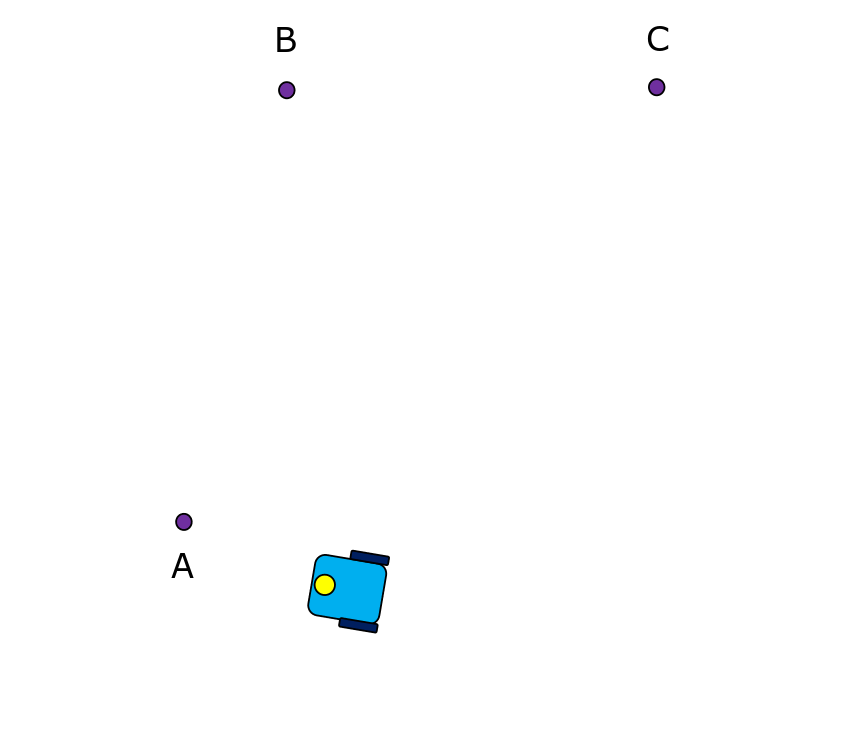
\includegraphics[scale=0.3]{./images/slam_example1}
\caption[Sample environment for a SLAM example]{A simple environment for SLAM\footnotemark}
\label{slam_example1}
\end{figure}
\footnotetext{Courtesy of Margarita Chli for the SLAM example figures}
The robot at its initial location (trivially taken as origin of the map to built), as shown in Figure~\ref{slam_example2}, observes landmark A in its field of view and takes a range measurement. The uncertainty associated with this measurement is represented by an ellipse as shown in Figure~\ref{slam_example3}, which is a 2D Gaussian. 
\begin{figure}
\centering
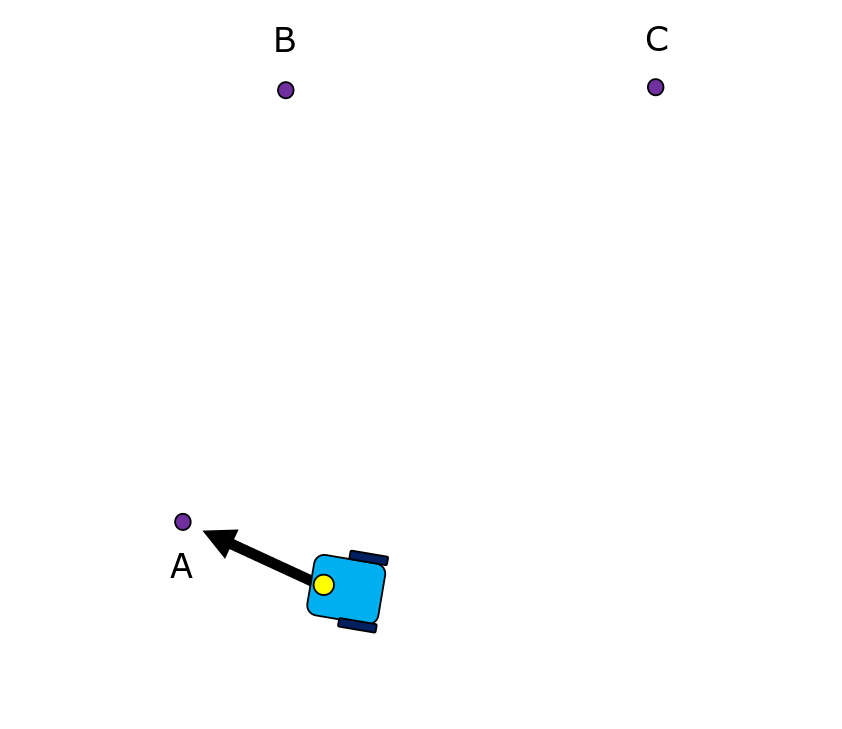
\includegraphics[scale=0.3]{./images/slam_example2}
\caption{First measurement of landmark A}
\label{slam_example2}
\end{figure}
\begin{figure}
\centering
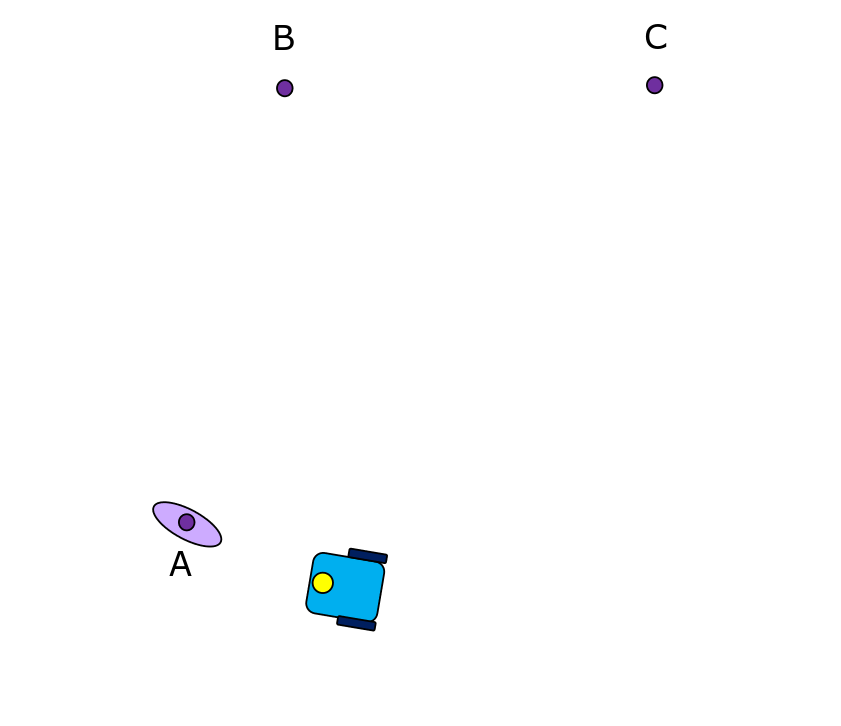
\includegraphics[scale=0.3]{./images/slam_example3}
\caption{Update of landmark position A}
\label{slam_example3}
\end{figure}

The robot begins to explore the environment after the update of landmark A into its memory. The uncertainty associated with its motion measurement from odometry is represented by a similar Gaussian as shown in Figure~\ref{slam_example4}. Due to the uncertainty in the robot's position or the path of the robot, subsequent range measurements of landmarks B and C are corrupted gradually as shown in Figure~\ref{slam_example5} and Figure~\ref{slam_example6}. Hence, the map built through the robot's sensors begin to drift due to this uncertainty.
\begin{figure}
\centering
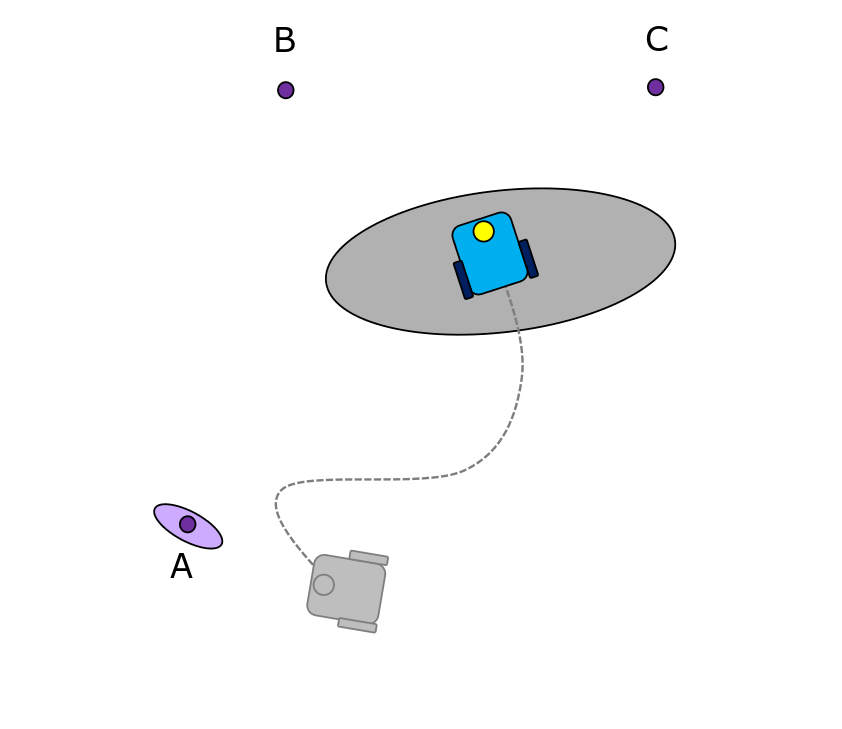
\includegraphics[scale=0.3]{./images/slam_example4}
\caption{Exploration of the environment}
\label{slam_example4}
\end{figure}
\begin{figure}
\centering
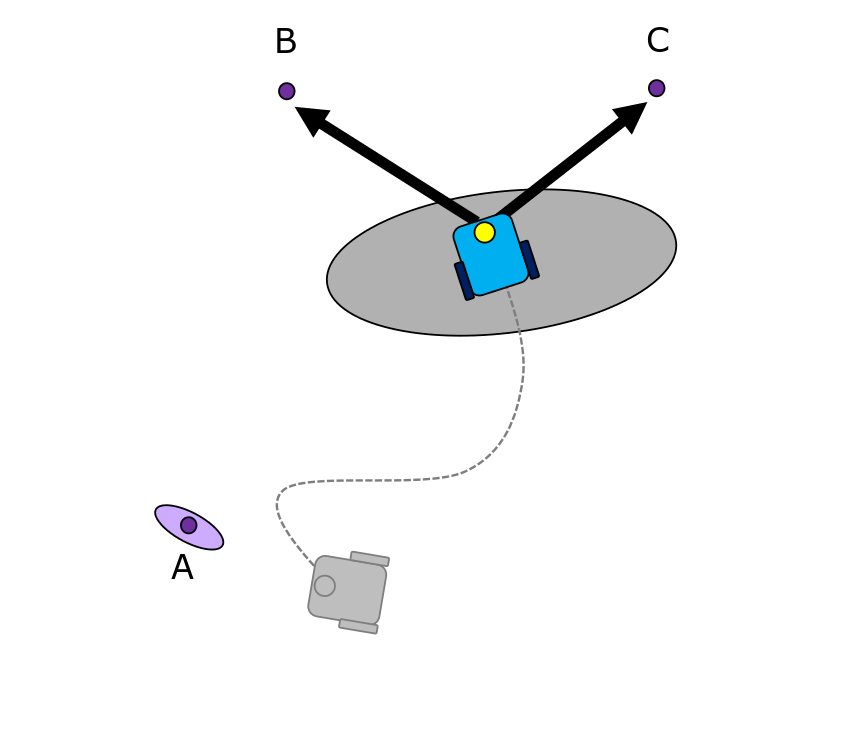
\includegraphics[scale=0.3]{./images/slam_example5}
\caption{Measurements of landmarks B and C}
\label{slam_example5}
\end{figure} 
\begin{figure}
\centering
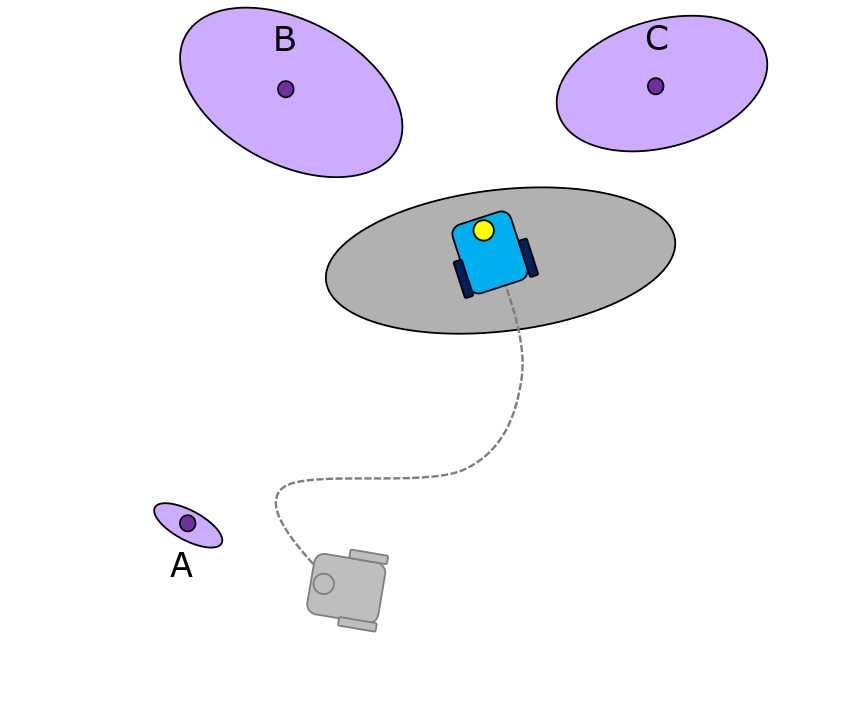
\includegraphics[scale=0.3]{./images/slam_example6}
\caption{Update of landmarks B and C}
\label{slam_example6}
\end{figure} 

The robot continues to explore with the error in the robot position or path begins to grow systematically. At certain point in time, the robot detects an old landmark as shown in Figure~\ref{slam_example8}. The robot compares a new measurement of that landmark with the old measurement and finds a mismatch between them. The main factor contributing to this problem is the error in the robot's current position which is corrected using the new measurement and the old updated estimate of landmark A. Since the entire set of landmark measurements were correlated due to the error in robot's path, all the landmarks get updated as a result. This step is especially called as loop closure problem and it is illustrated in Figure~\ref{slam_example9}.\hfill $\square$

\begin{figure}
\centering
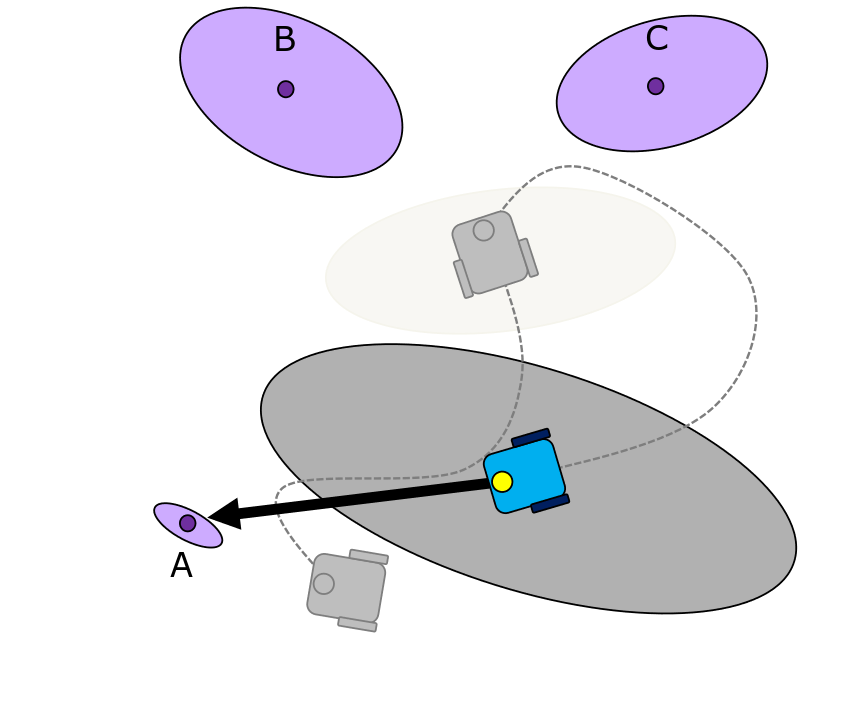
\includegraphics[scale=0.3]{./images/slam_example8}
\caption{Second measurements of landmark A}
\label{slam_example8}
\end{figure} 

\begin{figure}
\centering
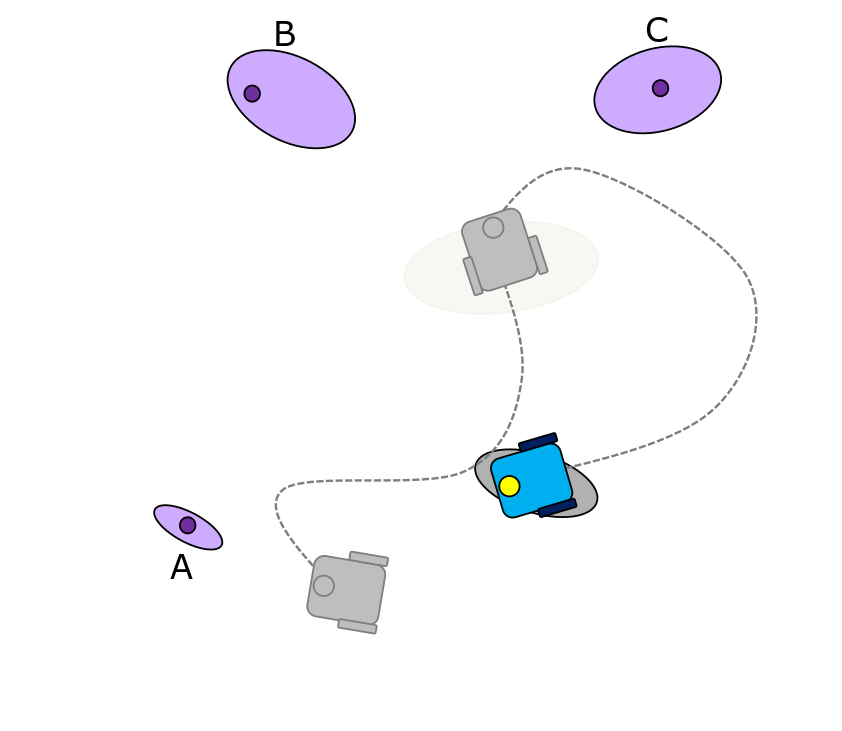
\includegraphics[scale=0.3]{./images/slam_example9}
\caption{Loop closure in SLAM}
\label{slam_example9}
\end{figure}
\label{slam_exmp}  
\end{exmp}

The illustration of \acs{SLAM} makes the problem more clear and gives an intuitive idea. A key factor affecting the estimates of the landmark positions was the error in the robot position or path and this factor bridges a correlation between the landmark estimates and robot position. Moreover, unlike the measurement noise, the error in the robot's pose has a systematic effect on the error in the map and as a result, the true map cannot be estimated without estimating the true path of the robot. This property gives rise to the chicken-egg nature of the SLAM problem. 

A probabilistic formulation of the SLAM problem is used for developing the SLAM algorithm which explicitly deals with the uncertainty in the problem. The probabilistic approach has received wide-spread attention due to their applicability in SLAM and has contributed to a separate dimension in the field of robotics called Probabilistic Robotics \cite{thrun2005probabilistic}. 

According to standard SLAM formulation, a robot executes control and accumulates observations, both corrupted by noise. Each control or observation, coupled with an appropriate noise model, can be thought of as a probabilistic constraint. As the robot explores through the environment, the network of constraints expand and get updated with re-observations. With re-observations, the constraints turn less uncertain and become increasingly rigid. In the limit of infinite observations and controls, the position of all map features become fully correlated. The SLAM problem is illustrated as a network of constraints in Figure~\ref{network_constraint}. For the case of structured environments like the rectilinear environment in the Figure, the landmarks are additionally correlated through geometric structure such as orthogonality.

\begin{figure}
\centering
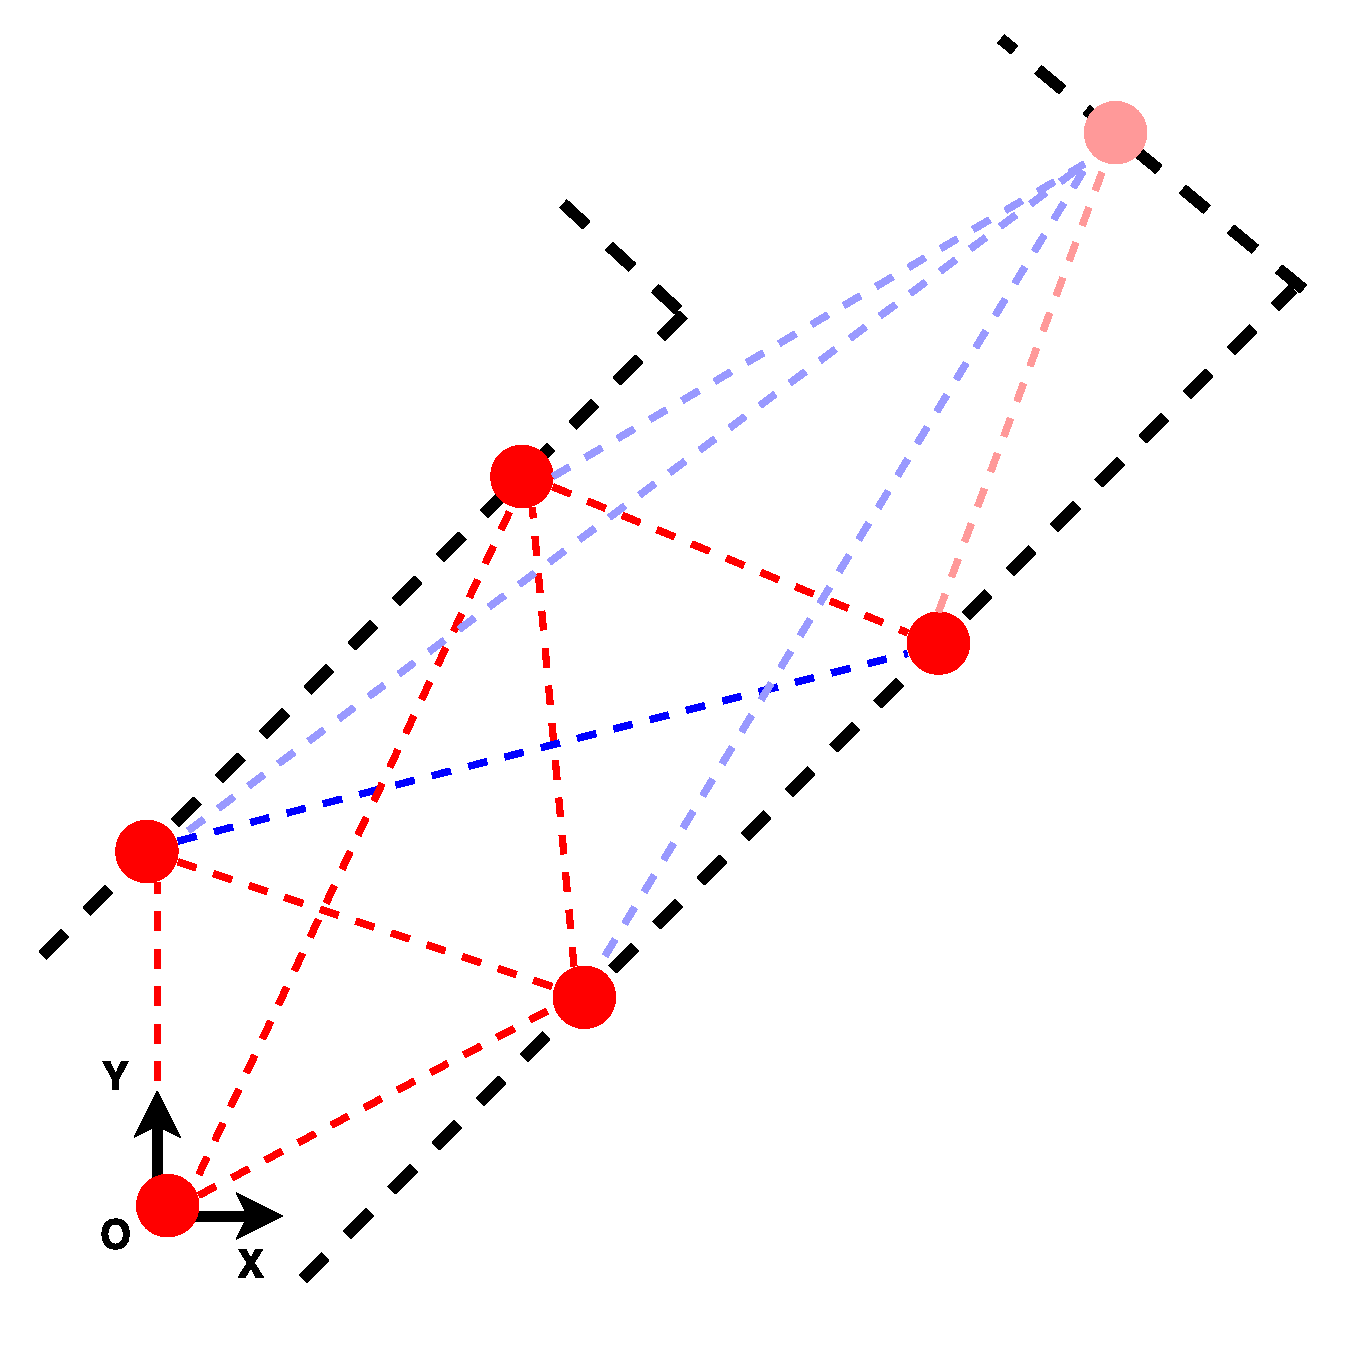
\includegraphics[scale=0.4]{./images/network_constraint}
\caption[Network of constraints in impact-based SLAM]{Network of constraints in impact-based SLAM; multiple observations of landmarks (dark red color) are constrained higher than the new landmarks (light red color). The blue lines represent the correlations through environment structure.}
\label{network_constraint}
\end{figure}  

A popular extension of the above formulation is posterior estimation of the SLAM problem. The objective is to estimate a probability distribution over the possible maps and robot poses, given the observations and controls. The distribution, referred to as SLAM posterior, can be written as:
\begin{equation}
p(s_t,m|z_{1:t},u_{1:t},c_{1:t})
\end{equation}
where \lsymb{$s_t$}{Robot pose at time $t$} is the robot pose at time $t$ and \lsymb{$m$}{Map of an environment} is the map of an environment. The variables \lsymb{$z_{1:t}$}{Time history of observations}, \lsymb{$u_{1:t}$}{Time history of control inputs} and \lsymb{$c_{1:t}$}{Time history of data associations} corresponding to the set of measurements, controls and data associations respectively and the posterior is conditioned upon them. The data association describes the mapping between a measurement $z_t$ and a landmark in $m$. The description of these variables will be explained in detail in the forthcoming chapter.

There does exists an alternative formulation which is suitable for computing the best possible map and robot pose. This approach is commonly called an offline optimization approach where a global nonlinear optimization is carried over a batch of measurements. This approach has gained popularity in the recent years by exploiting the sparsity in SLAM. 

The posterior approach seems desirable since it gives a distribution of possible solutions along with the uncertainty associated with it. This approach is robust in noisy environments since it explicitly considers the uncertainty factor in the problem. At first glance, the optimization approach might seem simpler than the posterior approach, however by considering judicious assumptions about how the state of the world and robot evolves, the posterior computation can be more efficient. For example, consider the following recursive formula, known as Bayes filter, which computes the posterior at time $t$.
\begin{equation}
\begin{split}
p(s_t,m|z_{1:t},u_{1:t},c_{1:t})\,&=\,\eta\,p(z_t|s_t,m,c_t)\cdot \\
&\cdot\int p(s_t|s_{t-1},u_t)\,p(s_{t-1},m|z_{1:t-1},u_{1:t-1},c_{1:t-1})ds_{t-1} 
\end{split}
\label{bayes_filter}
\end{equation}

The above integrand cannot be computed in closed form for a general probability distribution. However, if a particular form of distribution is considered such as Gaussian, a closed loop solution is indeed possible. Variants of Bayes filter such as Kalman filter and Particle filter are discussed in forthcoming section.  

\section{State-of-the-Art solutions} \label{sec::state_art}
Achieving a solution to the SLAM problem was one of the most demanding research in mobile robotics literature for past two decades. SLAM has been regarded as a prerequisite for a robot to be truly autonomous and from decades of research, a practical solution is found to be indeed possible. 

A consistent solution is achieved only when a complete set of correlations are propagated through a sequence of measurements and controls. However, the efficiency of computation ($\mathcal{O}(n^2)$, $n$ being the state dimension) became an obstacle for achieving a practical solution. Researchers \cite{montemerlo2002conditional} later came up with more robust SLAM algorithms which are practically efficient in terms of computational and memory requirements through exploitation of structure in SLAM. This estimation technique is called as online estimation since measurements are processed as they arrive.

The two state-of-the-art approaches for SLAM using online estimation techniques are Extended Kalman Filter-SLAM and Particle filter-SLAM. The two approaches are formulated and discussed in the following sections.

\subsection{Extended Kalman filter-SLAM} \label{sec::ekfslam}
\acf{EKF} is a parametrized representation of Bayes filter which approximates SLAM posterior as a multivariate Gaussian distribution over all features in the map and robot pose. The parametrized representation describes the probability distribution uniquely using mean $\mu$ and covariance $\Sigma$.

The state transition probability is described using the motion model of the robot,
\begin{equation}
p(s_t|s_{t-1},u_t)\Longleftrightarrow s_t~=~f(s_{t-1},u_t)~+~w_t,
\end{equation}
where \lsymb{$f(\cdot)$}{State transition model} corresponds to the robot's motion model, $s_t$ and $u_t$ represent the robot pose and control input respectively at time instant \lsymb{$t$}{Continuous time index}, and \lsymb{$w_t$}{Process noise} represents an additive, zero-mean, uncorrelated Gaussian noise with covariance \lsymb{$Q_t$}{Process noise covariance at time $t$}.

In a similar manner, the observation model is described using the following form-
\begin{equation}
p(z_t|s_t,m)\Longleftrightarrow z_t~=~h(s_t,m)~+~v_t,
\end{equation}
where \lsymb{$h(\cdot)$}{Observation model} describes the geometry of the observation, $z_t$ denotes observation and \lsymb{$v_t$}{Observation noise} represents another additive, zero-mean, uncorrelated Gaussian noise with covariance \lsymb{$R_t$}{Observation noise covariance}.

The state vector for EKF-SLAM  is usually defined as an augmented state of robot pose $s_t$ and observed landmarks $m$. For the observation of a new landmark, a new state is defined using the inverse of observation model, and then append to the original state vector. A feature-based representation is used here where the individual observed point landmarks are defined either through their location or pose. Hence, a map is represented as a set of landmark positions or poses, $m=\begin{bmatrix}m_1, m_2, \cdots, m_N\end{bmatrix}$. Additional details on map representation will be discussed in Section \ref{sec::env_rep}.

The standard EKF method can be applied to compute the mean \gsymb{$\mu_t$}{Mean of state estimate at time $t$} and the covariance \lsymb{$P_t$}{Covariance of state estimate at time $t$} given the measurements $z_{0:t}$ using a recursive update as shown below.

\textbf{Prediction step}
\begin{align}
\hat{s}_{t|t-1}&=f(\hat{s}_{t-1|t-1},u_t) \\
P_{t|t-1}&=\nabla f\cdot P_{t-1|t-1}\cdot\nabla f^T~+~Q_t
\end{align}
The gradient $\nabla f$ is the Jacobian of $f$ evaluated at the estimate $\hat{s}_{t-1|t-1}$.

\textbf{Update step}
\begin{align}
\begin{bmatrix} \hat{s}_{t|t} \\ \hat{m}_t \end{bmatrix}&=\begin{bmatrix} \hat{s}_{t|t-1} \\ \hat{m}_{t-1} \end{bmatrix}+K_t\cdot\left(z_t-h(\hat{s}_{t|t-1},\hat{m}_{t-1})\right) \\
P_{t|t}&=P_{t|t-1}-K_t\cdot S_t\cdot K^T_t \\
S_t&=\nabla h\cdot P_{t|t-1}\cdot \nabla h^T+R_t \\
K_t&=P_{t|t-1}\cdot\nabla h^T\cdot S^{-1}_t
\end{align}

The Kalman gain is denoted by \lsymb{$K_t$}{Kalman gain at time $t$} and innovation covariance is denoted by \lsymb{$S_t$}{Innovation covariance at time $t$}. The Jacobian \gsymb{$\nabla(\cdot)$}{Jacobian of a function} is evaluated with respect to state estimates at respective time instance. 

The above SLAM algorithm assumes that the correspondences of all the landmarks are known prior. SLAM algorithm with unknown correspondences will be detailed in Section \ref{sec::da}, which is a small addition to the existing EKF-SLAM algorithm. Moreover, it is assumed here that all the landmarks are initialized prior.

The prediction step propagates the mean and covariance of the belief in accordance to the motion model. This propagation step only affects the belief distribution associated with the robot pose. The landmarks of the map retain the same mean and covariance due to the static world assumption. 

In the update step, the observed landmark is updated using the innovation and Kalman gain. The Kalman gain is a matrix of size 3 by 3$N$+3, \lsymb{$N$}{Number of landmarks} being the number of landmarks. This matrix is usually not sparse and the information is propagated through the entire state estimate. The fact that the Kalman gain is fully populated for all state variables and not just for the observed landmark and robot pose is because of the correlations, that is observing the landmark does not just improve the position estimate of this very landmark but all the other landmarks as well. The situation is neatly depicted through the Example~\ref{slam_exmp}. Issues such as convergence, computational efficiency and data association have been addressed extensively in literature and a good survey discussing these issues is \cite{bailey2006simultaneous}. The issues specific to impact-based SLAM problem is discussed in Section~\ref{sec::challenges}.

\subsection{Particle filter-SLAM} \label{sec::pfslam}
With the above parametric form of estimation, a closed-form solution is obtained for SLAM. However, various issues such as computational efficiency and data association raised questions of implementing EKF-SLAM for large-scale environments. Meanwhile, the success of non-parametric estimation techniques such as particle filters and its variant, \acf{MCMC} have emerged as a core algorithm in Machine Learning. The direct applicability of particle filter to SLAM is intractable (Remark~\ref{pf_scale}) since they are subjected to the curse of dimensionality and a straightforward implementation of particle filter algorithm will be intractable due to the huge number of variables involved in the map. 
\begin{rem}
The computational requirement scales exponentially with the number of dimensions in a particle filter, as opposed to quadratic scaling of computations for a Gaussian update in an EKF. 
\label{pf_scale} 
\end{rem}

The conceptual breakthrough in the success of particle filters in SLAM was developed by \cite{montemerlo2002fastslam}. The probabilistic Markov chain property and conditional independence were best exploited in implementing a tractable version of particle filter-SLAM. Specifically, the full SLAM problem with known correspondences possess a conditional independence property between any two disjoint set of features in the map, given the robot trajectory. In other words, if the robot trajectory is known to be accurate, the features or landmarks can be estimated independently. The correlation property stressed through the covariance matrix in Gaussian filters is exploited here as a conditional independence relation. This structural observation will make it possible to apply a specific version of particle filters known as \acf{RBPF} to the SLAM problem. The RBPF version will be hereby simply addressed as particle filter-SLAM. The effect of this exploitation brings the tractability to the problem. Note that bringing tractability through approximation has their own downsides. For example, particle resampling will have a long term effect on the consistency of the filter \cite{bailey2006consistency} since the process noise (robot pose error) correlates the landmark estimates unlike standard estimation techniques where the error fades out with incorporation of measurements.

A naive implementation of the RBPF-SLAM requires $\mathcal{O}(MN)$ time, where $M$ is the number of particles in the filter and $N$ is the number of landmarks. A tree-based data structure of landmark representation can reduce the time complexity and memory requirements from linear scale to logarithmic scale $\mathcal{O}(M\log N)$, making it significantly faster than the state-of-the-art EKF-SLAM algorithm \cite{huang2011observability}. This had led to the success of particle filter-SLAM for a real-time implementation in large environments, and its contribution to Stanley car, DARPA \cite{thrun2006stanley}. Another useful property of particle filter-SLAM is data association decisions which is made on per-particle basis rather than the most likely particle. As a result, the particle filter can maintain posterior over multiple associations and helps approximating the full posterior $p(s_{1:t},m,c_{1:t}|z_{1:t},u_{1:t})$. This property of RBPF-SLAM makes it robust towards data association errors. 

Apart from the above favourable properties, ability of particle filter to represent an arbitrary distribution is a generic property and can be usefully exploited here. A non-Gaussian distribution can be easily represented through samples, and hence nonlinear motion models can be easily implemented even in situations when the pose uncertainty is known to be very high. 

Assuming a SLAM posterior distribution with known correspondences, the SLAM problem can be formulated as a joint posterior,
\begin{equation}
p(s_{1:t},m|z_{1:t},u_{1:t})
\end{equation}

The assumption of known correspondences takes into account of perfect data association decisions taken \textit{a-priori}. In case of unknown correspondences, the joint posterior includes another variable $c_{1:t}$ which is estimated using data association techniques. 

The full SLAM posterior can be factorized based on the conditional independence property or Rao-Blackwellization.
\begin{equation}
p(s_{1:t},m|z_{1:t},u_{1:t},c_{1:t})=p(s_{1:t}|z_{1:t},u_{1:t},c_{1:t})\cdot\prod_{n=1}^N p(m_n|s_{1:t},z_{1:t},u_{1:t},c_{1:t})
\label{rbpf_fastslam}
\end{equation}

This factorization leads to a problem of estimating posterior over the robot path and $N$~problems of estimating $N$~landmark locations conditioned on the robot trajectory. The factorization is exact and it is based on the assumption that the robot trajectory is known to be accurate. The independence assumption also holds valid when the landmarks are randomly placed in the environment or the environment is unstructured. The factorization in the particle filter-SLAM is illustrated in Figure~\ref{FastSLAM_DBN}.
\begin{figure}
\centering
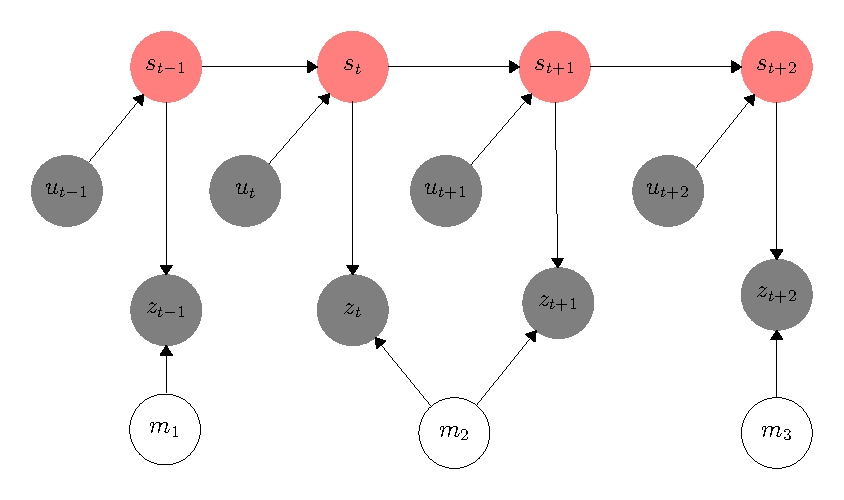
\includegraphics[scale=0.9]{./images/fsm}
\caption[Dynamic Bayesian Network graph of SLAM]{SLAM problem as a Bayes network graph. The control and measurements (gray shaded nodes) render conditional independence in mapping once the entire robot path (red shaded nodes) is known.}
\label{FastSLAM_DBN}
\end{figure}

The path estimate $p(s_{1:t}|z_{1:t},u_{1:t},c_{1:t})$ can be computed efficiently from the sample space since a good approximation of the posterior can be found even in the presence of nonlinear motion models. The landmarks are separately estimated using low dimensional EKFs, and since the landmark estimates are conditioned on the robot path, each particle in the particle filter has its own map of landmark estimates.

The particle filter-SLAM algorithm maintains a set of particles, $Y_t$, of size $M$ and the $k^{\text{th}}$ particle is denoted as $Y_t^{[k]}$. The $k^{\text{th}}$ particle is described systematically as a robot pose (or path) estimate $s^{[k]}_t$ augmented with a set of Gaussian feature estimates as shown below. 

\begin{equation}
Y_t^{[k]}=\left\langle s_t^{[k]}, \mu_{1,t}^{[k]}, \Sigma_{1,t}^{[k]}, \dots, \mu_{N,t}^{[k]}, \Sigma_{N,t}^{[k]} \right\rangle
\label{psf}
\end{equation}  

\textbf{Path estimation}

The particle filter-SLAM samples a new pose $s_t$ in accordance with the $k^{\text{th}}$ particle from the motion model,
\begin{equation}
s_t^{[k]}\sim p(s_t|s_{t-1}^{[k]},u_t)
\end{equation}
where $u_t$ is the current control action and $s_{t-1}^{[k]}$ is the posterior estimate of the robot pose at time $t-1$, residing in the $k^{\text{th}}$ particle. The resulting sample is appended to a temporary particle set which contains the propagated particles at time $t$.

As the previous particle set $Y_{t-1}$ is distributed according to the posterior at $t-1$, the temporary particle set is distributed according to $p(s_t|z_{t-1},u_t,c_{t-1})$. This distribution is referred to as proposal distribution in particle filter. 

After generating $M$ new particles this way, the new posterior set $Y_t$ is obtained from the temporary set by drawing particles (with replacement) with a probability proportional to its importance weight,
\begin{equation}
w_t^{[k]}=\frac{\text{target distribution}}{\text{proposal distribution}}=\frac{p(s_t^{[k]}|z_{1:t},u_{1:t},c_{1:t})}{p(s_t^{[k]}|z_{t-1},u_t,c_{t-1})}.
\label{imp_wt}
\end{equation}     
 
The importance weights for all the particles account for the mismatch between the proposal and the target distribution. This can be illustrated in Figure~\ref{sample_weighting}. The exact calculation of this importance weight will be discussed below. 
\begin{figure}
\centering
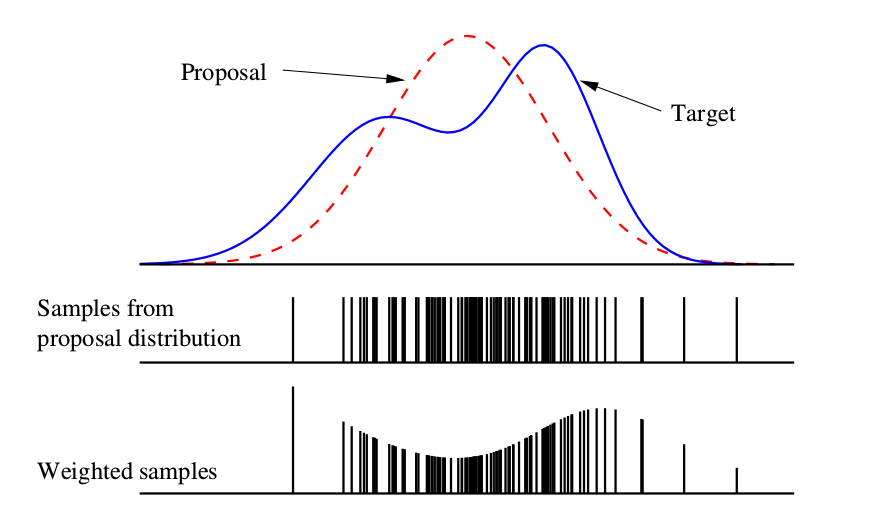
\includegraphics[scale=0.4]{./images/sample_weighting}
\caption[Importance Sampling in a particle filter]{Importance Sampling step in a particle filter \cite{thrun2005probabilistic}}
\label{sample_weighting}
\end{figure}

Note that only the latest pose estimate is used to compute the future posterior in Equation~\ref{imp_wt} according to Markov assumption (see Definition~\ref{def1}). The improvement in computational efficiency as a result of this assumption will be seen in the forthcoming chapter.

\textbf{Landmark location estimation}

From the particle description (\ref{psf}), each particle maintains a set of Gaussians (mean and covariance estimate) for landmarks in the map. For planar environment with point landmarks, the mean $\mu_{i,t}^{[k]}$ is a 2-element vector and the covariance $\Sigma_{i,t}^{[k]}$ is a $2\times 2$ matrix for a landmark. These variables are propagated with the incoming measurements.

For a landmark whose correspondence does not relate to the measurement, the corresponding Gaussian is unchanged.
\begin{equation}
\left\langle \mu_{i,t}^{[k]}, \Sigma_{i,t}^{[k]} \right\rangle=\left\langle \mu_{i,t-1}^{[k]}, \Sigma_{i,t-1}^{[k]} \right\rangle
\end{equation}

Otherwise, the corresponding Gaussian is updated using Bayes' product.
\begin{equation}
p(m_{c_t}|s_{1:t},z_{1:t},c_{1:t})=\eta\cdot p(z_t|s_t,m_t,c_t)\cdot p(m_{c_t}|s_{1:t-1},z_{1:t-1},c_{1:t-1})
\label{bayes_produp}
\end{equation}    

This update is implemented using an EKF where the observation model $z_t=h(s_t,m)$ is linearized at the current system state.

\textbf{Calculation of importance weights}

The problem of calculating the importance weights is continued from (\ref{imp_wt}) as follows,
\begin{align}
w_t^{[k]}&\propto\frac{p(s_t^{[k]}|z_{1:t},u_{1:t},c_{1:t})}{p(s_t^{[k]}|z_{t-1},u_t,c_{t-1})} 
\\
\intertext{From Bayes' product,}
&\propto p(z_t,c_t|s_t^{[k]},z_{1:t-1},u_{1:t},c_{1:t-1}), \\
\intertext{and using Markov assumption,}
&\approx\int p(z_t|m_i^{[k]},s_t^{[k]},c_{1:t})\cdot p(m_i^{[k]})\cdot dm
\end{align}

The above integral can be computed as a finite sum due to a discrete representation of a map. The probabilities can be convolved as Gaussians using a linearized observation model and a Gaussian posterior of the map. For a detailed proof of the importance weight calculation, refer~\cite{montemerlo2002fastslam}.

In the above formulation, the particles are sampled according to the motion model using the current control input and then weighted according to its likelihood with the incoming measurement. The particles are then resampled to obtain the posterior distribution. One of the practical issues in SLAM is degeneracy in evolution of posterior distribution over time. The degeneracy is observed in a scenario where the motion model is less accurate as compared to the observation (measurement) model. The proposal distribution using the less accurate motion model generates a large spectrum of samples (or particles) out of which a small subset has a high likelihood with the incoming measurements. After resampling, only few particles from the proposal distribution survive after resampling (see Figure~\ref{fastslam2}) and this can result in loss of particle diversity or degeneracy. The state-of-the-art version of particle filter-SLAM, \cite{montemerlo2007fastslam}, avoids this problem by incorporating measurements into the motion model for a better prediction estimate, at the expense of intensive computation.
\begin{figure}
\centering
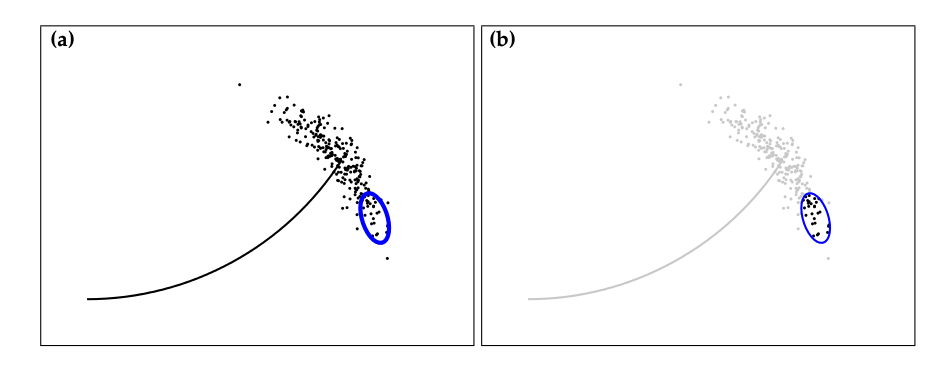
\includegraphics[scale=0.4]{./images/fastslam2}
\caption[Modified proposal distribution for SLAM]{(a) Mismatch between proposal and posterior distribution, and (b) the contribution of samples after resampling \cite{thrun2005probabilistic}.}
\label{fastslam2}
\end{figure}

\section{Research objectives} \label{sec::thesis_statement}
With the appropriate introduction, the thesis work will focus on a minimalistic approach to achieve \acl{SLAM}. The main research problem for the thesis is to accomplish SLAM with an impact-based approach using minimal sensing information. 

In this dissertation, I will advance the following thesis:
\begin{center}
\noindent\parbox{0.9\textwidth}{\it An impact-based approach to Simultaneous Localization and Mapping with minimal sensing information is proposed and implemented.}
\end{center}

The feature extraction in impact-based SLAM is sparse in nature and it may require a long exploration to map the environment. For example, an omnidirectional camera requires a single frame of data to map a simple rectangular environment while it may take many collisions for the impact-based approach. The thesis work is extended to use multiple robots to map the environment and merge the individual maps from the robots. This map-merging problem has a short exploration time and can also ensure a more consistent map of the environment.

\section{Thesis contributions} \label{sec::thesis_contributions}
In this thesis, a probabilistic formulation of the impact-based SLAM problem is addressed with a suitable robot model and an environment representation. A unicycle motion model is used to approximate the robot motion in the environment with the effect of collisions on robot motion modelled through a Finite State Machine, and a suitable rectilinear environment representation is used for incorporating measurements from the environment. 

\begin{center}
{\it A new efficient map representation is proposed for rectilinear environments.}
\end{center}

The new representation models walls of a rectilinear environment as histograms and this representation is compared with the traditional point landmark representation. The new representation might share a similarity with occupancy maps since both involve discretizing the state space. However, the new map representation rasterizes only the useful part (for recording collision measurements) of the map, thereby giving it an edge over the occupancy maps in terms of memory usage and consistency. The suitability and efficiency of map representation is addressed in detail along with an implementation of the most suitable one.

\begin{center}
{\it \centering The impact-based SLAM algorithm is developed using probabilistic formulation and is implemented on the practical setup.}
\end{center}

An impact-based SLAM algorithm is developed using the robot and environment model with collision and odometry information as inputs and robot's path and map as outputs. A particle filter-SLAM is preferred over the existing state-of-the-art SLAM algorithms due to favourable properties relating to the impact-based mapping as follows. Firstly, the poor pose distribution of the robot can be easily represented through a set of particles rather than a smooth Gaussian representation. Secondly, the growth of map information can be well represented through a discrete distribution because of the availability measurement information.
 
A clear layout is made for the impact-based SLAM algorithm detailing the key steps for obtaining the solution. Simulation results validate the feasibility of SLAM solution and comparisons between various landmark representations are analysed. Issues such as convergence, computational effort and consistency of the solution are addressed. The impact-based SLAM algorithm is implemented on a practical setup using Sphero robot and is extended to multiple robot-SLAM. 

\begin{center}
{\it The SLAM problem is accomplished with multiple robots as a map-merging problem for achieving a higher consistency.}
\end{center}

The robots individually build a local map of the environment and at some point, the maps are fused together which has a higher consistency than the single robot-SLAM and is achieved with a lower exploration time.

\section{Outline} \label{sec::outline}
This thesis report comprises of five chapters, including the current chapter. Chapters~\ref{chap::problem}~and~\ref{chap::solution} give the necessary theoretical background for impact-based SLAM with simulation results, followed by Chapter~\ref{chap::implementation} implementation of the developed algorithm. Chapter~\ref{chap::conclusion} summarizes the thesis with a discussion and recommendations for future work. 

A detailed outline of the thesis is as follows,

\textbf{Chapter~\ref{chap::problem}} formulates SLAM in a probabilistic fashion suitable for impact-based SLAM. The motion model and observation model is defined for the impact-based approach along with a suitable environment representation. Various challenges to the SLAM problem are addressed.

\textbf{Chapter~\ref{chap::solution}} presents an impact-based SLAM algorithm using Rao-Blackwellized particle filter. Suitable illustrations and simulation results support the developed algorithm, followed by map-merging problem using multiple robots.

\textbf{Chapter~\ref{chap::implementation}} provides the results of SLAM experimentation with Sphero robots. The robot and its sensing modalities are discussed. The experimental results for both single robot and multiple robot-SLAM are provided.

\textbf{Chapter~\ref{chap::conclusion}} summarizes the thesis with a discussion and recommendations for future work.  
\chapter{Problem description} \label{chap::problem}
{\it \centering In this chapter, the impact-based SLAM problem is described from a probabilistic viewpoint in Section~\ref{sec::formulation}. The essentials for building an accurate SLAM solution are a robot motion model and an environment representation. Section~\ref{sec::robotmodel} details the various motion models for the SLAM problem suitable for specific scenarios. Various environment representations suitable for rectilinear environments are discussed in Section~\ref{sec::env_rep} along with the proposed histogram maps. Section~\ref{sec::challenges} addresses various challenges relevant to the impact-based SLAM problem.}

\section{Notations}
In the impact-based SLAM problem, the Sphero robot collides with the walls of a given rectilinear environment randomly. The collision information, along with odometry through dead-reckoning, from the robot can infer the pose of a landmark. The odometry gives the position of collision while the collision information is used for calculation of landmark orientation. The collision is detected in Sphero when there is a sudden deceleration in either or both of the robot's coordinate axes X and Y. The wall orientation $\phi$ can be inferred from the collision information with respect to the robot's orientation \gsymb{$\theta$}{Robot orientation} by measuring the change or peak of impact along each coordinate axis. The dependence is shown below,
\begin{equation}
\phi-\theta = \arctan\left(\frac{a_x}{a_y}\right),
\end{equation}
where $a_x$ and $a_y$ represent the accelerometer reading at the highest peak of impact or the power of impact along the coordinate axis X and Y respectively. Further information about collision detection can be found in Section~\ref{sec::sphero} of Chapter \ref{chap::implementation}. 

At time instant \textit{t}, following quantities are defined:
\begin{description}
\item[$s_t:$] pose of the robot, containing position and orientation information
\item[$u_t:$] control input vector, containing velocity and heading, applied at time instant $\textit{t}-1$ to get the pose $s_t$
\item[$m_i:$] $i^{th}$ landmark position or pose
\item[$c_t:$] measurement correspondence at time $t$
\item[$z_t:$] measurement/observation from robot at time $t$
\end{description}

The time history of a variable $s$ is denoted as $s_{0:t}$. The correspondence of a landmark to an incoming measurement is called as data association and it is crucial for any SLAM problem. This step is very important since standard estimators are prone to divergence for incorrect associations.

\section{Probabilistic formulation}  \label{sec::formulation}
The probabilistic formulation of the SLAM describes the problem in the most certain way possible with uncertainty dealt explicitly. The uncertainty in the SLAM problem, crucial for tractability, has been modelled in few of the most common forms. For example, in the case of Extended Kalman filter, the uncertainty is modelled as a Gaussian while the particle filter models the uncertainty as a set of particles.

There are two main forms of the probabilistic SLAM problem, which are equally important in their own aspects and have their own pros and cons. One is known as the online SLAM problem, involving estimation of posterior over momentary pose along with the map. The online version is an incremental algorithm which discards past measurements and controls once they have been processed. Using the above notations, online SLAM is defined as the following posterior:
\begin{equation}
p(s_t,m|z_{1:t},u_{1:t},c_{1:t})
\end{equation}
If the set of data associations is known, the posterior becomes simple: 
\begin{equation}
p(s_t,m|z_{1:t},u_{1:t})
\end{equation}

A convenient way to describe a probabilistic SLAM algorithm and its structure is through a \ac{DBN}. Expressing SLAM through a DBN highlights its temporal structure as a Markov chain. A Bayesian network is a graphical model describing a stochastic process as a directed graph. The graph has one node for each variable in the process and a directed edge between two nodes models the conditional dependence between them. For further information on Bayesian networks, refer \cite{koller2009probabilistic}. For example, the online SLAM problem as a DBN is depicted in Figure~\ref{online_SLAM}. 

\begin{figure}
\centering
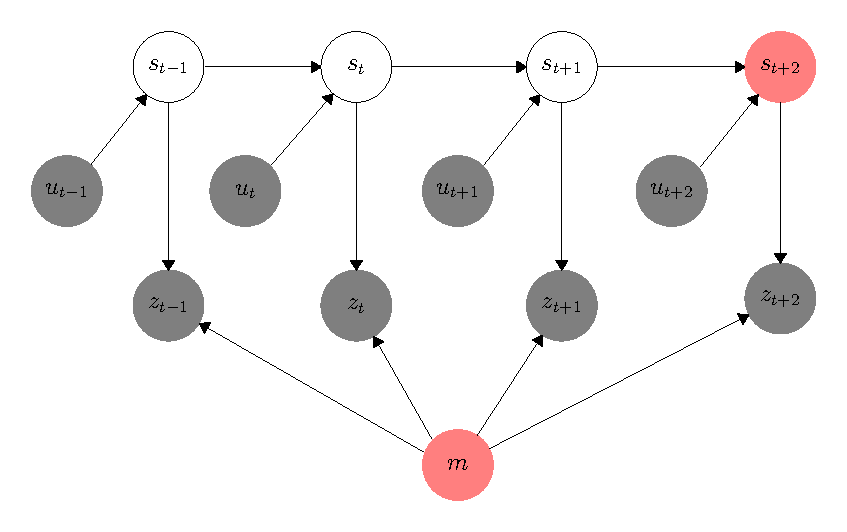
\includegraphics[scale=0.9]{./images/fsm2}
\caption[Dynamic Bayesian Network graph of online SLAM problem]{Graphical model of online SLAM problem. The online SLAM estimates a posterior over the current robot pose and map. The red shaded nodes are estimated in this problem given the gray shaded nodes.}
\label{online_SLAM}
\end{figure}

\begin{figure}
\centering
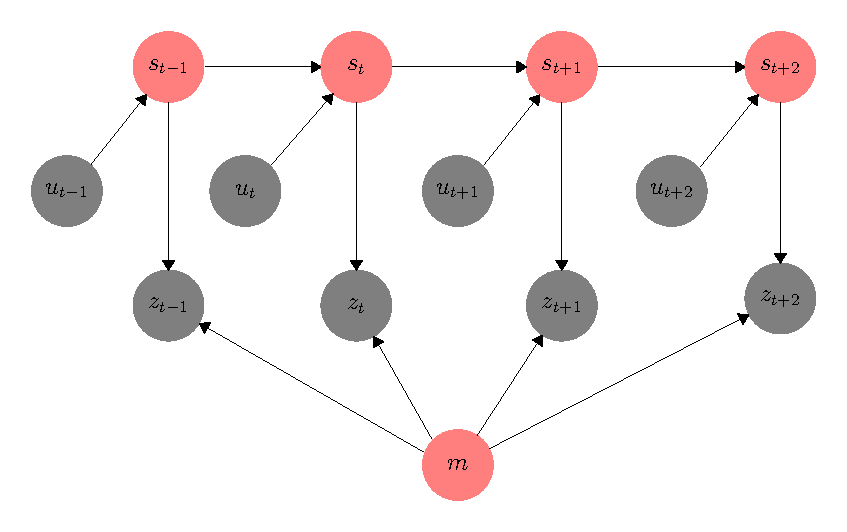
\includegraphics[scale=0.9]{./images/fsm3}
\caption[Dynamic Bayesian Network graph of full SLAM problem]{Graphical model of full SLAM problem. The full SLAM estimates a posterior over the entire robot trajectory and map. The red shaded nodes are estimated in this problem given the gray shaded nodes.}
\label{full_SLAM}
\end{figure}

The other form of probabilistic SLAM is called full SLAM problem which calculates the posterior over the entire pose trajectory along with the map. The data association set is assumed to be known.
\begin{equation}
P(s_{1:t},m|z_{1:t},u_{1:t})
\end{equation}

The full SLAM problem as a DBN is depicted in Figure~\ref{full_SLAM}. The initial condition $s_0$ is assumed to be known in both the SLAM forms and is removed from the conditioning term for simplicity in notations.

The full version of the SLAM problem involves the entire measurement and state information which results in an enormous computational complexity introduced by the huge data, while the online version is more suitable for practical applications such as navigation since the measurements are processed as they arrive. However, the full SLAM results in a more accurate and consistent estimate since it models the entire set of correlations between the measurements and robot trajectory which is neglected in the online version.

In general, a recursive solution to the SLAM problem is desirable since measurements can be processed as they arrive. The joint posterior is updated using Bayes' Theorem with the help of a state transition model and an observation model which are individually affected by control input and observation respectively. 

A state transition model describes a systematic update to the pose of the robot in terms of a probability distribution of the form-
\begin{equation}
P(s_t|s_{t-1},u_t).
\end{equation} 

The state transition model is assumed to be a Markov process in which the next state of the robot depends only upon the previous robot pose and recent control action. This structure is important for reducing the computational complexity of the SLAM problem.  

The observation model describes the probability of making an observation given the robot pose and map of the environment- 
\begin{equation}
P(z_t|s_t,m).
\end{equation}

If the landmark is a new one, it has to be appended to a set of new landmarks. The landmark initialization function is defined as the inverse of observation model. 

The state transition model and observation model characterizes the connectivity of the Bayesian network through a recurrent pattern as shown in Figures~\ref{online_SLAM}~and~\ref{full_SLAM}. The state transition model is represented by the edges connecting the state variable which represents the probability of state variable at that time instant. Similarly, the observation model models the probability of performing an observation given that the robot is at a location in the map. Expressing SLAM as DBN highlights its temporal structure, and this formalism is exclusively suited to describe SLAM as a filtering problem. 

The recursive Bayesian update is carried out using the state transition and observation model in a two-step recursive procedure, more popularly called as Bayes filter. The Bayes filter can be derived from the SLAM posterior as follows.

\textbf{Bayes filter derivation}

The SLAM posterior can be rewritten using the Bayes' rule as given below.
\begin{equation}
p(s_t,m|z_{1:t},u_{1:t},c_{1:t}) = \eta\cdot p(z_t|s_t,m,z_{1:t-1},u_{1:t},c_{1:t})\cdot p(s_t,m|z_{1:t-1},u_{1:t},c_{1:t})
\end{equation}

The first term in the product, $\eta$, is a normalizing constant in the Bayes' rule. The fact that the current measurement $z_t$ is solely a function of pose of the robot $s_t$, map $m$ and data association $n_t$ can be exploited to simplify the above product. 
\begin{equation}
p(s_t,m|z_{1:t},u_{1:t},c_{1:t}) = \eta\cdot p(z_t|s_t,m,,c_{1:t})\cdot p(s_t,m|z_{1:t-1},u_{1:t},c_{1:t})
\end{equation}

Using the theorem of total probability to condition the last term of the product on pose at time $t-1$,
\begin{equation}
= \eta\cdot p(z_t|s_t,m,c_{1:t})\cdot\int p(s_t,m|s_{t-1},z_{1:t-1},u_{1:t},c_{1:t})\cdot p(s_{t-1}|z_{1:t-1},u_{1:t},c_{1:t})\cdot ds_{t-1}
\end{equation}

The leftmost term in the integral can be expanded using conditional probability theory.
\begin{equation}
\begin{split}
= \eta\cdot p(z_t|s_t,m,,c_{1:t})\cdot\int p(s_t|m,s_{t-1},&z_{1:t-1},u_{1:t},c_{1:t})\cdot p(m|s_{t-1},z_{1:t-1},u_{1:t},c_{1:t})\cdot \\
&\cdot p(s_{t-1}|z_{1:t-1},u_{1:t},c_{1:t})\cdot ds_{t-1}
\end{split}
\end{equation}

The first term of the above product can be simplified assuming the state propagation is a Markov process, hence $s_t$ is only a function of $s_{t-1}$ and $u_t$. 
\begin{equation}
\begin{split}
= \eta\cdot p(z_t|s_t,m,,c_{1:t})\cdot\int p(s_t|s_{t-1},u_t)&\cdot p(m|s_{t-1},z_{1:t-1},u_{1:t},c_{1:t})\cdot \\
&\cdot p(s_{t-1}|z_{1:t-1},u_{1:t},c_{1:t})\cdot ds_{t-1}
\end{split}
\end{equation}

Also, the last two terms in the integral product can be combined together using Bayes' product.
\begin{equation}
\begin{split}
p(s_t,&m|z_{1:t},u_{1:t},c_{1:t}) = \\
&\eta\cdot p(z_t|s_t,m,,c_{1:t})\cdot\int p(s_t|s_{t-1},u_t)\cdot p(s_{t-1}, m|z_{1:t-1},u_{1:t},c_{1:t})\cdot ds_{t-1}
\end{split}
\end{equation}

Since the process is causal in such a way where the current input $u_t$ and data association $c_t$ provide no new information about the previous state $s_{t-1}$ or map m without the latest observation $z_t$, they can be dropped from the rightmost term of the integral. The result obtained turns out to be a recursive formula for computing the SLAM posterior at time $t$ given the SLAM posterior at time $t-1$, motion model $p(s_t|s_{t-1},u_t)$ and observation model $p(z_t|s_t,m,c_t)$.

The state transition probability assumes a Markov propagation in system states for computational efficiency. The Markov assumption states that the probability distribution of the next state depends upon the previous state and not on the sequence of states that preceded it. This requires a crucial assumption that the system is characterized by a complete state.
\begin{defn}
A complete state is defined as a characterization of a system which can be the best predictor of the future. If any state is sufficient to describe a future state with a given input, the past states can be neglected in calculations.
\label{def1}
\end{defn} 

The error from the latter can be compensated by inflating the covariance information of the corresponding process. This assumption is quite successful in practical SLAM algorithms, especially in particle filter-SLAM algorithm where the pose error is factored out. The problem in the former case can be removed by considering a modified complete state of the system.

The accuracy of the prediction step is increased by conditioning the map state in state transition probability $p(s_t|s_{t-1},u_t,m)$. Inclusion of map state tends to remove poor state hypotheses in Bayes filter. A similar statement is used in the particle filter-SLAM algorithm where measurements are included in the prediction step to reduce degeneracy of particle filter. However, computation of this probability can be cumbersome and efficient approximations are used. Let us briefly derive it using Bayes' rule.
\begin{equation}
p(s_t|u_t,s_{t-1},m)\cdot p(m|u_t,s_{t-1}) = p(m|s_t,u_t,s_{t-1})\cdot p(s_t|u_t,s_{t-1})
\end{equation}

As $p(m|u_t,s_{t-1})$ can be considered a constant $\eta$, a desired approximation of $p(m|s_t,u_t,s_{t-1})$ is used as $p(m|s_t)$.
\begin{equation}
p(s_t|u_t,s_{t-1},m) = \eta\cdot p(m|s_t)\cdot p(s_t|u_t,s_{t-1})
\end{equation}

A similar Bayes' rule product is obtained with a different normalization constant $\hat{\eta}$.
\begin{equation}
p(s_t|u_t,s_{t-1},m) = \hat{\eta}\cdot p(s_t|m)\cdot p(s_t|u_t,s_{t-1})
\end{equation}

Inclusion of $p(s_t|m)$ can improve the accuracy of the prediction step through reduced degeneracy. For example, as the robot comes close to a wall, it is not good to represent a probability of robot being present on the wall or the other side. Hence, an inclusion of map can remove this problem. A detailed proof of the modified prediction step or proposal distribution is provided in Appendix~\ref{mod_prop}.  

Various SLAM algorithms quite differ on the representation of these probability distributions and type of the sensors used. The following sections describe these distributions that are suitable for the impact-based SLAM. The importance and manipulation of these recursive steps will be explained in detail in future.

\section{Robot model} \label{sec::robotmodel}
The goal of a probabilistic robot model is to accurately model the specific types of uncertainty that exists in robot actuation and perception. In practice, the exact model seems to be less important than the fact that some provisions for uncertain outcomes are provided in the first place. Accurately modelling the robot is important to control the robot dynamics but in situations where certain dynamics of the robot are not excited much as part of the problem, it is not useful to model them. For the impact-based SLAM, the Sphero robot moves in straight lines between collisions and rotates around itself at the collision point.  Hence, a unicycle model is sufficient to explain the behaviour of this motion and the unmodeled dynamics can be accounted as uncertainty. In case of motion planning, more accurate geometric models such as SO(3) are needed and will be considered as future work of this thesis.

\subsection{Motion model}
There are two specific probabilistic motion models for the Sphero mobile robot. Both the models are somewhat complimentary in the type of motion information being processed. The first model, called velocity motion model, assumes that the motion data specifies the velocity and heading commands given to the robot. The second model, called odometry motion model, assumes that the motion information is provided through the odometry. The latter is more accurate than the former for a simple reason that error in the unmodelled robot kinematics are not accounted  and the information is available post-the-fact. The velocity motion model is most suitable for autonomous robots as it incorporates the robot motion model which is essential for motion planning. 

The two models used in SLAM algorithms are shown in Figures~\ref{vel_model}~and~\ref{odom_model}. 

\begin{figure}
\centering
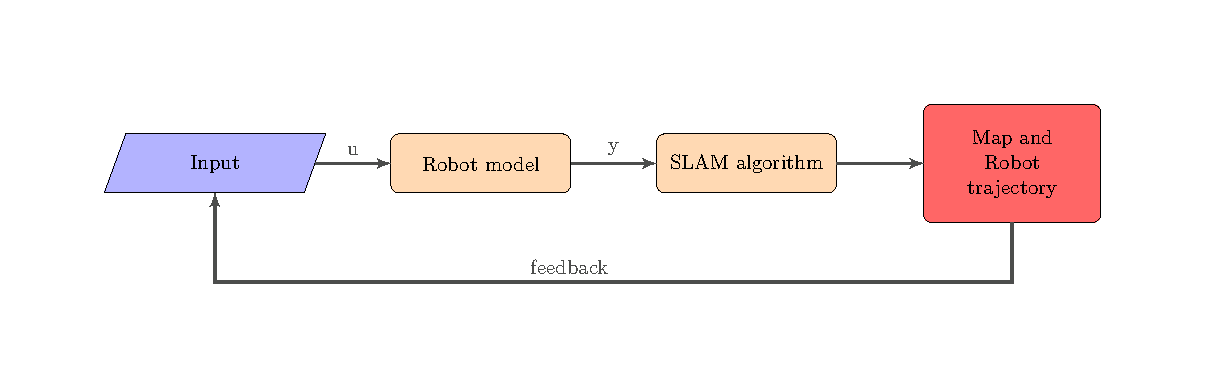
\includegraphics[scale=0.75]{./images/vel_model}
\caption[Velocity model]{Velocity model for SLAM with planning; $\text{u}$ denotes control input and y denotes the measurement including the odometry. The feedback enables planning in SLAM.}
\label{vel_model}
\end{figure}

\begin{figure}
\centering
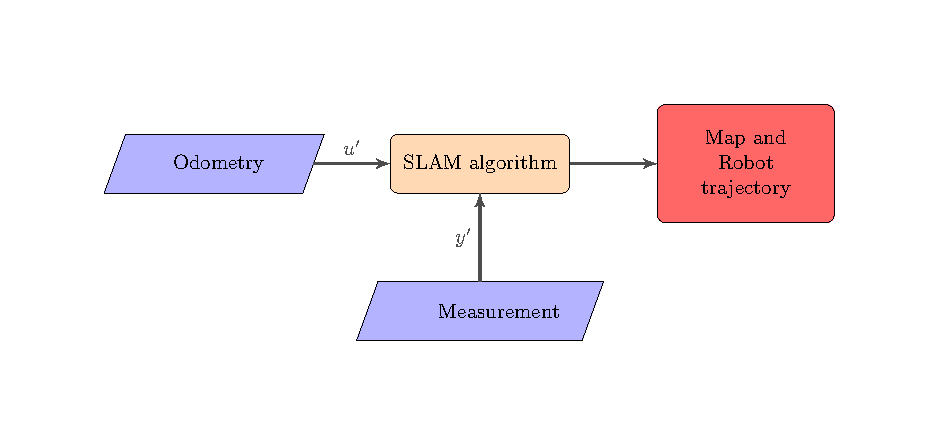
\includegraphics[scale=0.75]{./images/odom_model}
\caption[Odometry model]{Odometry model for SLAM; $u'$ denotes odometry input and $y'$ denotes the collision measurement}
\label{odom_model}
\end{figure}

\subsubsection{Velocity motion model}
A sampling based approach is used to compute the state transition probability from a given state $s_{t-1}=[x_{t-1},y_{t-1},\phi_{t-1}]$ and control input $[\text{speed},\text{head}]$. The time from $t-1$ to $t$ is denoted $dt$ and during this period, the control input is constant. The samples are randomly generated (\textbf{gauss}) from a Gaussian distribution either using Central Limit Theorem or a more efficient Box-Muller technique. After the sampling step, the pose is propagated through a unicycle robot model to get a new pose. The computation of the state transition probability is shown in Algorithm~\ref{alg_vel}.

\begin{figure}
\begin{algorithm}[H]
\caption{Sampling from velocity motion model}\label{alg_vel}
\begin{algorithmic}[1]
\BState \textbf{Input}: $s_{t-1}=[x_{t-1},y_{t-1},\phi_{t-1}]$, $[\text{speed},\text{head}]$, $dt$
\Procedure{Sampling}{}
\State $\mathrm{speed} = {\bf gauss}(\text{speed},\alpha_1\sqrt{speed})$
\State $\mathrm{head} = {\bf gauss}(\text{head},\alpha_2\sqrt{head})$
\EndProcedure
\Procedure{Propagation}{}
\State $\mathrm{angle} = (head + \phi_{t-1})\%(2\pi)$
\State $x_t = x_{t-1} + \mathrm{speed}\cdot dt\cdot{\bf cos}(\mathrm{angle})$
\State $y_t = y_{t-1} + \mathrm{speed}\cdot dt\cdot{\bf sin}(\mathrm{angle})$
\State $\phi_t = \phi_{t-1} + \mathrm{speed}\cdot dt\cdot{\bf sin}(\mathrm{head}/L)$
\State \textbf{return} $s_t=[x_t,y_t,\phi_t]$
\EndProcedure
\end{algorithmic}
\end{algorithm}
\caption[Sampling algorithm using velocity motion model]{New pose $s_t=[x_t,y_t,\phi_t]$ is sampled from old pose $s_{t-1}=[x_{t-1},y_{t-1},\phi_{t-1}]$ with a sample time $dt$ using controls $[\text{speed},\text{head}]$ from a robot of wheel base $L$.}
\end{figure}

\subsubsection{Odometry motion model}
Odometry measurements are obtained from the IMU of Sphero robot through integration of accelerometer data and gyroscopic data (called as dead-reckoning). A similar sampling approach is adopted for the odometry based approach but without the robot model. The input to the sampling algorithm is previous robot pose estimate $s_{t-1}=[x_{t-1},y_{t-1},\phi_{t-1}]$ and the odometry reading, $u=[[\bar{x}_{t-1},\bar{y}_{t-1},\bar{\phi}_{t-1}],[\bar{x}_{t},\bar{y}_{t},\bar{\phi}_{t}]]$. The propagation is more simple than the previous where the propagation step is described with separate translational and rotational movements as shown in Figure~\ref{odometry_motion}. The propagation approach is suitable for very small movements since larger time steps might result in robot jumping over features which cannot be explained through the robot's motion model. The computation of state transition probability is shown in Algorithm~\ref{alg_odom}.

\begin{figure}
\centering
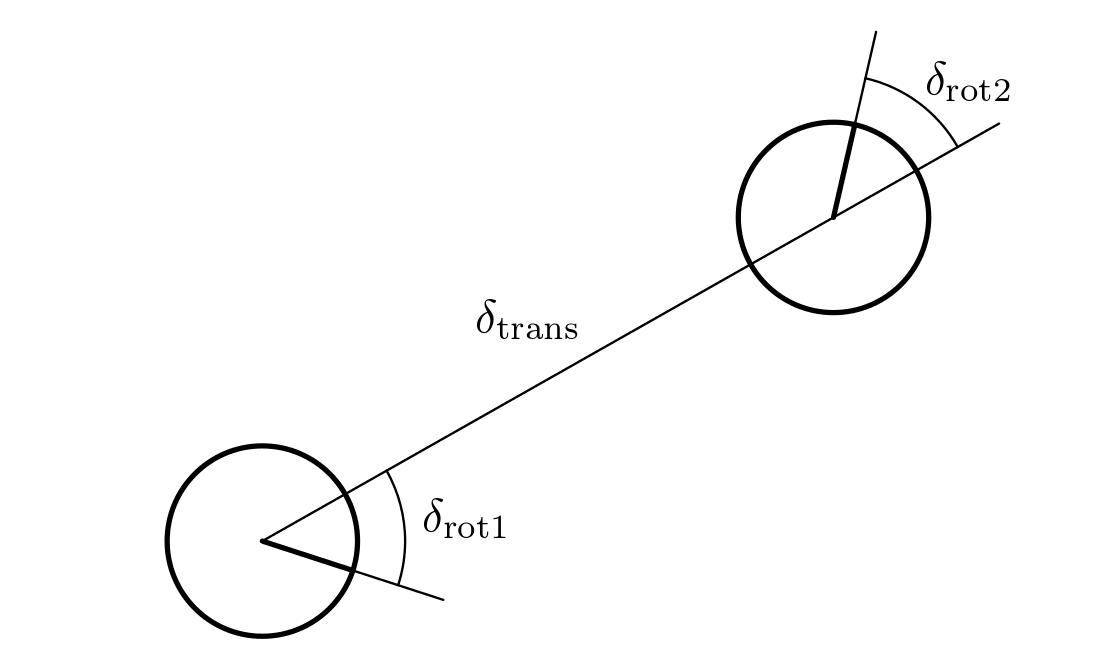
\includegraphics[scale=0.2]{./images/odometry_motion}
\caption[Approximation of robot motion in odometry model]{The robot motion is approximated by a sequence of rotation $\delta_{\text{rot1}}$, translation $\delta_{\text{trans}}$ and rotation $\delta_{\text{rot2}}$ \cite{thrun2005probabilistic}.}
\label{odometry_motion}
\end{figure}

\begin{figure}
\begin{algorithm}[H]
\caption{Sampling from odometry motion model}\label{alg_odom}
\begin{algorithmic}[1]
\BState \textbf{Input}: $s_{t-1}=[x_{t-1},y_{t-1},\phi_{t-1}]$, $[[\bar{x}_{t-1},\bar{y}_{t-1},\bar{\phi}_{t-1}],[\bar{x}_{t},\bar{y}_{t},\bar{\phi}_{t}]]$
\Procedure{Controls}{}
\State $\delta_{\text{rot1}} = {\bf atan2}(\bar{y}_{t}-\bar{y}_{t-1},\bar{x}_{t}-\bar{x}_{t-1}) - \bar{\phi}_{t-1}$
\State $\delta_{\text{trans}} = \sqrt{\strut(\bar{y}_{t}-\bar{y}_{t-1})^2+(\bar{x}_{t}-\bar{x}_{t-1})^2}$
\State $\delta_{\text{rot2}} = \bar{\phi}_{t} - \bar{\phi}_{t-1} - \delta_{\text{rot1}}$
\EndProcedure
\Procedure{Sampling}{}
\State $\hat{\delta}_{\text{rot1}} = {\bf gauss}(\delta_{\text{rot1}},\alpha_1\delta_{\text{rot1}}+\alpha_2\delta_{\text{trans}})$
\State $\hat{\delta}_{\text{trans}} = {\bf gauss}(\delta_{\text{trans}},\alpha_3\delta_{\text{trans}}+\alpha_4(\delta_{\text{rot1}}+\delta_{\text{rot2}}))$
\State $\hat{\delta}_{\text{rot2}} = {\bf gauss}(\delta_{\text{rot2}},\alpha_5\delta_{\text{rot2}}+\alpha_6\delta_{\text{trans}})$
\EndProcedure
\Procedure{Propagation}{}
\State $x_t = x_{t-1} + \hat{\delta}_{\text{trans}}\cdot{\bf cos}(\phi_{t-1}+\hat{\delta}_{\text{rot1}})$
\State $y_t = y_{t-1} + \hat{\delta}_{\text{trans}}\cdot{\bf sin}(\phi_{t-1}+\hat{\delta}_{\text{rot1}})$
\State $\phi_t = \phi_{t-1}+\hat{\delta}_{\text{rot1}}+\hat{\delta}_{\text{rot2}}$
\State \textbf{return} $s_t=[x_t,y_t,\phi_t]$
\EndProcedure
\end{algorithmic}
\end{algorithm} 
\caption[Sampling algorithm for odometry motion model]{New pose $[x_t,y_t,\phi_t]$ is sampled from old pose $s_{t-1}=[x_{t-1},y_{t-1},\phi_{t-1}]$ through a set of translation $\delta_{\text{trans}}$ and rotations $\delta_{\text{rot1}}$ and $\delta_{\text{rot2}}$. The last input is the consecutive odometry measurement from time $t-1$ to $t$.}
\end{figure}

\subsection{Observation model}   
The measurements available from the Sphero robot are odometry and collision measurements. The odometry from the IMU provides the robot pose through dead-reckoning and the correlation between the robot position from odometry and landmark position is straightforward since for the impact-based SLAM, the robot is present at the absolute location of collision (except for an offset which can be corrected in the map). The nonlinear relation between the collision information $\dfrac{a_x}{a_y}$, robot orientation $\theta$ and landmark orientation $\phi$ is shown below,
\begin{equation*}
\phi-\theta = \arctan\left(\frac{a_x}{a_y}\right)
\end{equation*}

The resulting observation model of a landmark $l$ is shown,
\begin{equation*}
y_l = \begin{bmatrix}x_r \\ y_r \\ c_r\end{bmatrix} = \begin{bmatrix}
x_l \\ y_l \\ \tan(\phi-\theta),
\end{bmatrix}
\end{equation*}
where $(x_l,y_l)$ denotes the landmark position, $(x_r,y_r)$ denotes the robot odometry and $c_r$ denotes the collision information. Note that the robot orientation $\theta$ is also a part of the measurement. A probabilistic version can be obtained from the observation model much similar to the sampling approach in motion model.
 
\section{Environment representation} \label{sec::env_rep}
A suitable environment representation is needed to build a map of the environment and use the map to estimate the robot trajectory. The accuracy of a map representation is directly correlated with the accuracy of the SLAM solution, and care is taken to represent the environment in the best possible way. 

In the case of impact-based SLAM, the given environment is an indoor world which comprises of rectilinear walls. The orthogonality assumption in walls is crucial for orientation correction for the robot. In addition, equal corridor width in the environment is a common assumption in indoor environments for correcting the position of the robot \cite{jensfelt2001approaches}. Additional assumptions such as boundary length are taken for building a map to ensure consistency if needed. 

The most suitable representations of an indoor environment are point landmarks, line representations and occupancy maps. The first is more simple than the other while the last involves more book-keeping. The later representation is more useful for the case of planning, and its variants are in use for the Google autonomous car. The line representation is suitable for a SLAM problem with a range-and-bearing sensor. The suitability of a map representation is deeply correlated with the data association (refer \ref{sec::da}) used for SLAM. Suitable environment representations for the impact-based SLAM problem are presented below.

\subsection{Point landmarks}
The point landmarks are described using pose information, or in other words, position and orientation (though mathematically, it is not appropriate for a point to be described using orientation). For the case of impact-based SLAM, the collision information has to be encoded in such a way to initialize and update corresponding landmarks for each and every collision. 

The point landmark representation is the most preferred representation in literature for analysis. The map is defined as a set of point landmarks where each landmark $m_i$ is defined by its pose and possible signatures. 
\begin{equation}
m = \begin{bmatrix}m_1 & m_2 \cdots & m_N\end{bmatrix}
\end{equation}
The simplest description of a point landmark is by its position $m_i=\begin{bmatrix}x_i & y_i\end{bmatrix}^T$. Additional components such as landmark signatures (e.g.\ color, texture) can be added to improve the description. 

For a 3-dimensional pose description of a point landmark, the uncertainty associated is also 3-dimensional in nature and can be modelled as a multivariate Gaussian.
\begin{equation}
\mathcal{N}\left(\begin{bmatrix}x_i \\ y_i \\ \phi_i \end{bmatrix},\begin{bmatrix}\sigma_{xx} & \sigma_{xy} & \sigma_{x\phi} \\ \sigma_{xy} & \sigma_{yy} & \sigma_{y\phi} \\ \sigma_{x\phi} & \sigma_{y\phi} & \sigma_{\phi\phi}\end{bmatrix}\right)
\end{equation}

For the case of impact-based SLAM problem, the use of point landmark is insufficient to completely represent the environment since the environment is rather more descriptive than point landmark representation. In addition, even if SLAM is carried out for a simple corridor environment, new landmarks are created for every collision and it is very rare that the robot touches the same landmark again. 

The above situation can however be avoided with two possible solutions-
\begin{enumerate}
\item The uncertainty associated with each landmark can be increased such that close collisions could be regarded as a single landmark. However, this can result in overestimation or a highly conservative estimate, and result in an inaccurate solution. This situation is exemplified in Example~\ref{example1}.  
\item The spatial information of the wall can be taken into account for clubbing collisions on the same wall. This technique involves taking only uncertainty along the orthogonal direction since orthogonal direction of uncertainty can be reduced from collision updates. However, the associated result was found to be poor since the environment information is not completely encoded, as exemplified in Example~\ref{example2}.
\end{enumerate}

A more suitable representation is required for a better description of the indoor environment as point landmarks were no more suitable. The data association results tend to fail a lot with these representations and hence, more complex representations are needed to better suit the environment and the algorithm. A new representation is required to suit a rectilinear environment for impact-based SLAM as well as address the issues of point landmark representation.

\begin{exmp} {\it Consider the Sphero robot mapping a corridor environment. The robot moves in a straight line between consecutive collision and the uncertainty associated with each collision is modelled as a Gaussian. The collision information is encoded as a point landmark and the associated algorithm is detailed.}

\qquad In standard EKF-SLAM, landmark pose is a component of mean of the multivariate Gaussian and associated uncertainty is maintained as sub-covariance of the Gaussian. A landmark is created from a measurement that does not correspond (nearest-neighbour gating) to any old landmark and updated if the corresponding landmark has a higher likelihood. Note that the association of point landmarks to measurements in this example holds for any data association algorithm in literature.

This approach is found to be less suitable for point landmarks since new landmarks are created for every collision within walls and there are no EKF updates. Hence, the associated uncertainty grows unbounded and there is no convergence in the solution. This can be illustrated in Figure~\ref{ex1_pl}. 

\begin{figure}
\centering
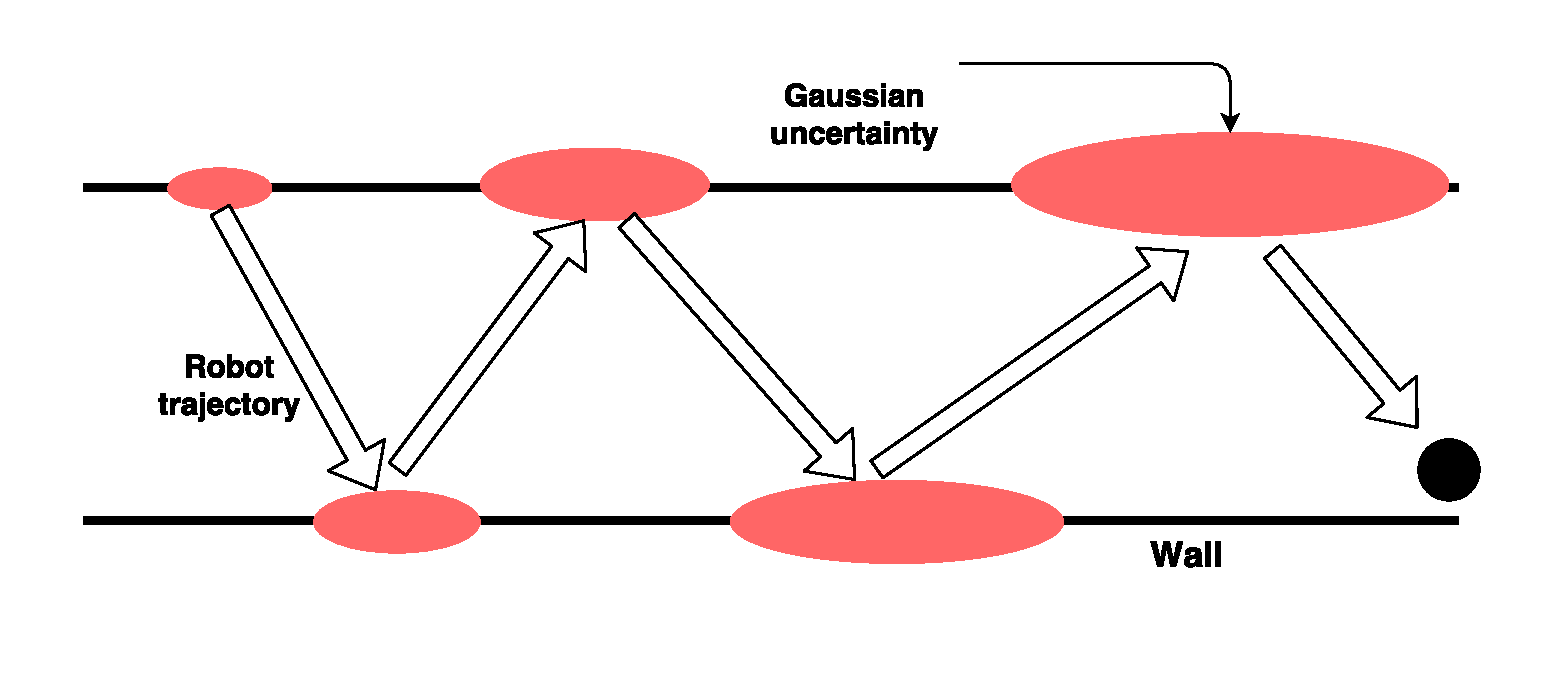
\includegraphics[scale=0.5]{./images/ex1_pointlandmark}
\caption[A simple point landmark representation]{New landmarks are created for collisions on the same wall. The robot coordinate frame is same as map coordinate frame.}
\label{ex1_pl}
\end{figure}  

In this example, five landmarks are created rather than two landmarks. The state vector of EKF-SLAM as a result becomes
\begin{equation}
x=\begin{bmatrix}x_r \\ y_r \\ \phi_r \\ m_1 \\ m_2 \\ m_3 \\ m_4 \\ m_5 \end{bmatrix}
\end{equation}

The size of state is found to increase linearly in the number of collisions and the uncertainty correspondingly grows unbounded. 

A suitable approach to overcome this issue is to go for scaled or inflated representation of uncertainty \cite{julier2003stability} such that close-by landmarks of the same wall can have lower Mahalonobis distance. The scaled representation is illustrated in Figure~\ref{ex1_scalepointlandmark} .
\begin{figure}
\centering
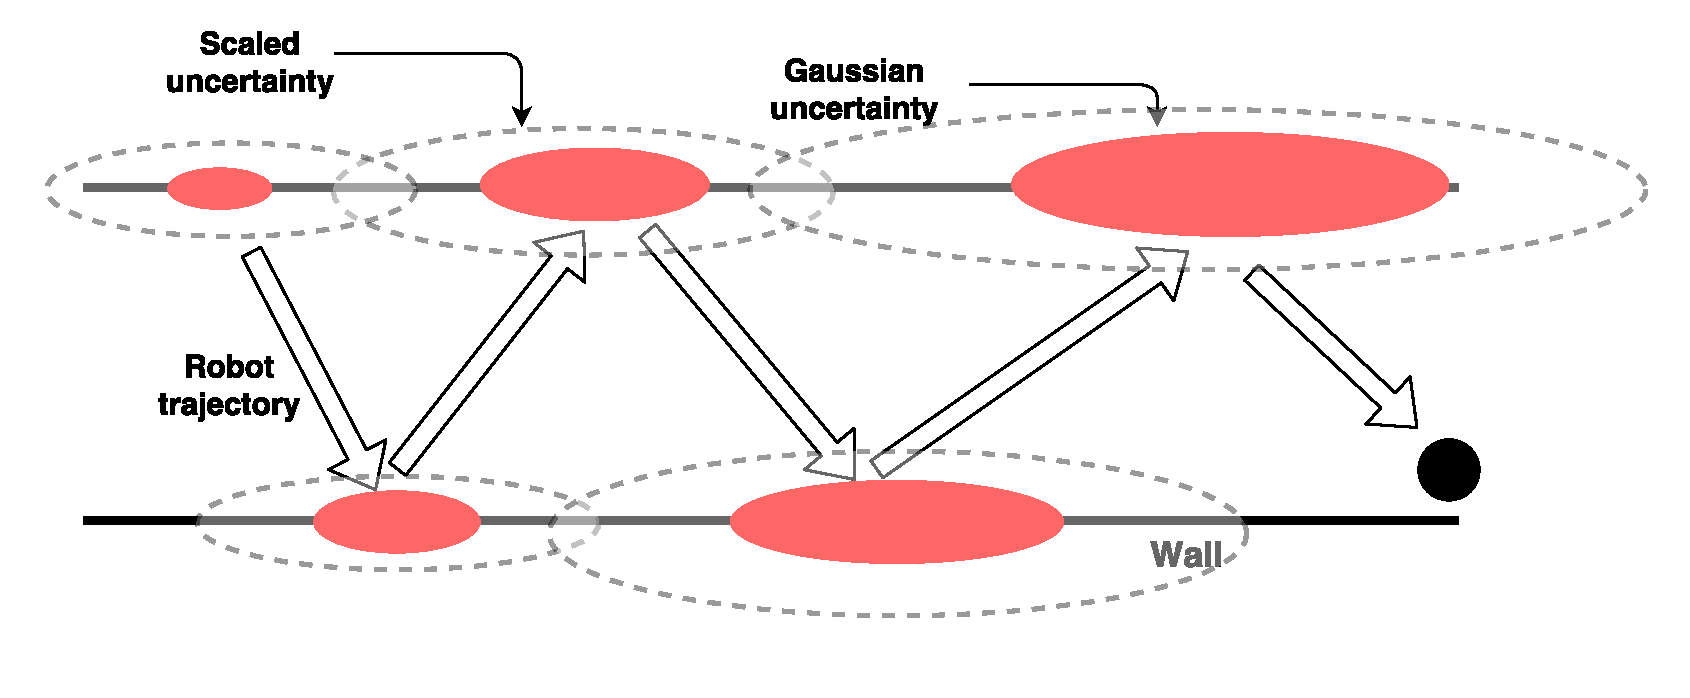
\includegraphics[scale=0.5]{./images/ex1_scalepointlandmark}
\caption[Scaled representation of point landmarks]{Scaled uncertainty to improve data association over the same wall}
\label{ex1_scalepointlandmark}
\end{figure}  

The resulting EKF-SLAM state turns out to be
\begin{equation}
x=\begin{bmatrix}x_r \\ y_r \\ \phi_r \\ m_1 \\ m_2 \end{bmatrix}
\label{eq_state}
\end{equation}

Consistency of map via this approach might be achieved by inflating the covariance \cite{julier2003stability} but it is not clear how to quantify adequate inflation. Even though the representation may appear simple, this technique may result in an unbounded growth in covariance with a non-converging solution. This is due to partiality in the uncertainty updates along the unit normal direction of the wall, which is usual in rectilinear environments.\hfill $\square$
\label{example1}
\end{exmp}

\begin{exmp} {\it Consider a similar situation to Example~\ref{example1} where the robot collides along the walls of a corridor. Spurious landmark creation were avoided by inflating the covariance matrix to ensure a consistent solution for the map. However, the map structure can be taken into account to reduce the overall scaling of the uncertainty representation.} 

\qquad A reduced state representation of the landmark state is chosen for data association. Let X-axis denote the orthogonal direction to the wall and Y-axis denote the axis along the wall. As the Y-axis correspond to the same landmark along the wall direction, collisions on the same wall (Y-axis) also correspond to the same landmark. Hence, the X-axis coordinate and orientation (reduced state) can be used for data association since the Y-axis does not contribute to any useful information for data association. This introduces a bounded covariance for this reduced state representation. The uncertainty along the wall axis (Y-axis) can be reduced when a joint covariance representation of all the landmarks are maintained or a \acf{CI} update is used between neighbouring orthogonal landmarks for incorporating orthogonal measurement information (Refer Section~\ref{sec::single_slam}).

In addition, information about the geometric structure of the environment can be incorporated. Constraints such as equal corridor width, orthogonality in wall orientation and boundary length can be incorporated into EKF as zero-uncertainty measurements \cite{newman1999structure}. Addition of these measurements can reduce the growth of covariance and ensure consistency of the SLAM solution.

The corridor width $w$ in an usual indoor environment is assumed to be constant \cite{jensfelt2001approaches}. This structure can be exploited to reduce the uncertainty along the orthogonal direction to the wall. For example, the two walls, each parametrized as a hyperplane $a_i^Tx=b_i$ where $x$ can be same as Equation \ref{eq_state}, can model the equal width constraint as
\begin{equation}
y = w = a_1^T\cdot x-a_2^T\cdot x = b_1-b_2 
\end{equation}

The orthogonal assumption and boundary length can be incorporated in a similar fashion. This technique can avoid the spurious landmark creation but at the expense of additional computation complexity through a joint covariance or constraint incorporation using covariance intersection (as detailed in the next chapter). \hfill $\square$
\label{example2}
\end{exmp}

The last approach still has an important disadvantage (Example~\ref{example1}) which is poor representation of the environment. The information of wall mass is not represented anywhere in point landmarks. For example, the spatial information (wall mass) of a discontinuous wall (as illustrated in Figure~\ref{gaussian_wall}) cannot be properly modelled as a Gaussian and it requires a more elaborate representation such as occupancy map or particles. Moreover, if distant collisions of the same wall are clubbed as a single landmark, combinatorial possibilities can open up whether they correspond to the same landmark or not during the pruning step (door openings might be present in between two collisions on the same wall). 
\begin{figure}
\centering
\begin{subfigure}{0.5\textwidth}

\includegraphics[scale=0.4]{./images/actual_wall.png}
\caption{A one-dimensional wall with discontinuous mass along the wall}
\end{subfigure}
\begin{subfigure}{0.5\textwidth}
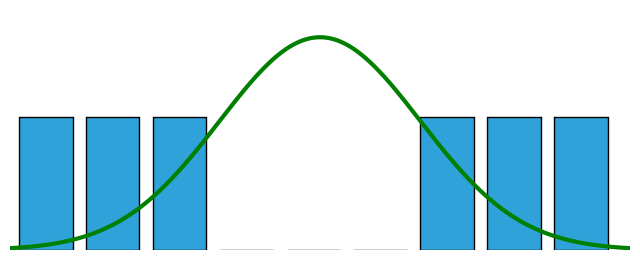
\includegraphics[scale=0.4]{./images/gaussian_wall.png}
\caption{Histogram and Gaussian representation of the wall mass}
\end{subfigure}
\caption[Spatial representation of a map information]{Spatial representation of wall mass information for a simple 1-D environment}
\label{gaussian_wall}
\end{figure}

The suitability of point landmarks for impact-based SLAM is also shown through simulations in the forthcoming chapter. 

\subsection{Occupancy maps}
A more popular and descriptive representation of a map than a point landmark is an occupancy grid where the entire map of an environment is rasterized into small cells. Each cell encodes the occupancy information and as a result, processing of information and estimation~\cite{thrun2005probabilistic} becomes more simple. For example, a cell $(i,j)$ is described by an occupancy state $x$ as,
\[ x(i,j) = \begin{cases}\,\,1 & \quad \text{if } \text{cell is occupied}\\ \,\,0 & \quad \text{if } \text{cell is free}\\ \,-1 & \quad \text{if } \text{cell is unknown} \end{cases} \] 

The occupancy map representation does not include any information about landmark signature and this map representation has been used extensively for planning and navigation since most of the planning algorithms favour a grid-structured map.

Occupancy maps can represent any arbitrary distribution at the expense of higher memory requirements. Impact-based SLAM in literature (\cite{fox2012tactile}, \cite{fox2012towards}) use an occupancy grid representation to account for the poor uncertainty distribution in impact-based mapping and SLAM. 

This thesis strikes a mid-level between a point landmark representation and occupancy map representation, by exploiting the advantages of both the approaches and aiding each other at shortcomings. Without further delay, the forthcoming section will detail the histogram representation of a map.

\subsection{Histogram maps} \label{sec::hist_map}
The thesis proposes a hybrid approach to an environment representation, much suitable for rectilinear environments. A landmark is represented using a point landmark description as well as with a histogram description. The landmark will turn out to be more descriptive than point landmarks and at the same time, the representation requires less of book-keeping compared to occupancy maps. Histogram representation of a 1D map has been used in literature \cite{thrun2005probabilistic} for pedantic purposes and not for a real-world implementation since occupancy maps turn out to be more descriptive.

Before getting deeper into histogram maps, a histogram is first defined.
\begin{defn} A histogram is a bar graph, illustrating the mapping $\mathcal{F}$ between finite domain $\mathcal{X}$ and its associated range $\mathcal{Y}=\mathcal{F}(\mathcal{X})$. A histogram can also represent a probability distribution where the domain represents a finite set of events and the range represents the associated probability of an event.
\end{defn}
Taking a more specific example (refer Figure~\ref{gaussian_wall}) such as a wall in an indoor environment for impact-based SLAM, the domain represents discretized wall location along the wall. The associated range describes the probability of mass information along the wall. To make it more clear, if X-axis describes the thickness of wall and Y-axis describes the wall length, the histogram is defined along the Y-axis and encodes information about the presence of wall. 

As said in the previous section, histogram maps strike a mid-level between point landmark representation and occupancy grid representation. For an indoor environment, each wall is described as a point oriented landmark where its pose is determined from the initial collision which lead to its inception. As a new landmark gets created, a new state describing its pose is augmented to the system state. In addition to the new state, a histogram with a finite support is also initialized for the corresponding landmark. The length of support is taken from the prior knowledge of the size of the environment. If the size of the environment is not perfectly known, an approximate bound is taken for the size and pruned later for a consistent map. 

Figure~\ref{gaussian_wall} illustrates the histogram representation of a discontinuous wall. The histogram can represent any discontinuous, non-Gaussian distribution and shares similarities with occupancy maps. This representation is aptly suited for impact-based SLAM since the collision information can be encoded into the histogram by propagating it through discrete Bayes filter while landmark pose is propagated using EKF similar to previous point representation. The discrete Bayes filter is a simple extension of continuous Bayes filter (refer Equation~\ref{bayes_filter}) where the integral gets converted to a finite sum. Spurious landmark creation is avoided using the approach followed in Example~\ref{example2}. The propagation of a histogram using discrete Bayes filter for an impact-based SLAM problem is shown in Example~\ref{ex24}.

\begin{exmp}
{\it Consider a wall in an one-dimensional world which contains an opening (open door). This can be illustrated in Figure~\ref{wall_example3}. A robot equipped with touch sensors, can move back and forth along the wall and make contacts at certain points. In addition, the position of a robot is given by a noisy odometry. A simple assumption is made here that there is no measurement noise associated with the touch sensors.}
\begin{figure}[H]
\centering

\includegraphics[scale=0.45]{./images/wall_example3.png}
\caption[A simple 1-D wall for impact-based mapping]{One-dimensional wall for impact-based mapping}
\label{wall_example3}
\end{figure}

\qquad The histogram is propagated as a probability distribution using discrete Bayes filter with a sequence of incoming measurements. The histogram represents the probability of occupancy along the wall and hence the initial distribution is assumed to be uniform. Two possible implementations of a collision update are Gaussian update and triangular update where the probability is computed at discrete points using these distributions. 

It is not necessary that histogram has to be declared as a probability distribution and use discrete Bayes' theorem for mapping the wall. A simple histogram update can be used where each cell contains a probability of occupancy (much similar to occupancy maps). Both the approaches of histogram representation have the same computational efficiency. Moreover, maintaining a collinear histogram also improves the consistency of the estimate along the wall. Figure~\ref{ex24coll_10} gives the difference between the two histogram update techniques for a single collision.

\begin{figure}
\centering
\begin{minipage}{0.45\textwidth}
\centering
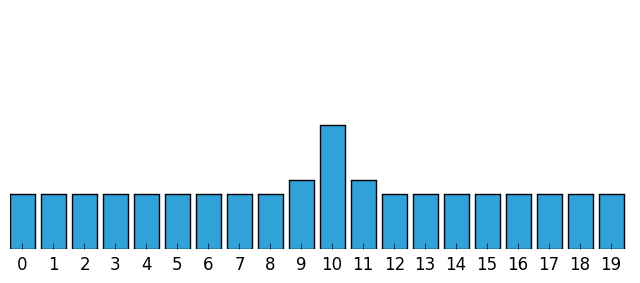
\includegraphics[scale=0.4]{./images/ex24/ex24coll10.png}
%\caption{Histogram as a probability distribution}
\end{minipage}
\begin{minipage}{0.45\textwidth}
\centering
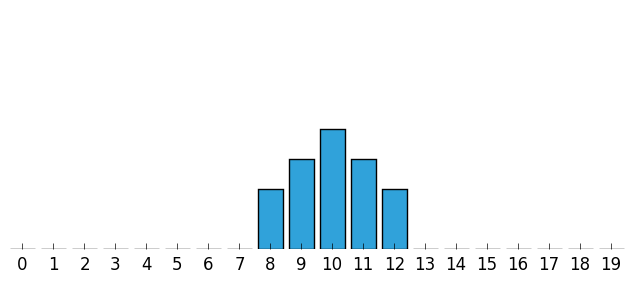
\includegraphics[scale=0.4]{./images/ex24/ex24coll10_1.png}
%\caption{A simple histogram update}
\end{minipage}
\caption[Histogram propagation of measurement information]{Propagation of histogram for an incoming measurement. The left histogram is propagated as a probability distribution whereas the right is a simple histogram update (not a probability distribution).}
\label{ex24coll_10}
\end{figure}

Figure~\ref{ex24_collisions} give a list of histogram updates along the wall, with collisions occurring according to the cell sequence $\left\lbrace 10,4,12,13,1,5,9,6,7,19\right\rbrace$. A triangular collision update is used here for simplicity. The corresponding map of the wall is shown for each collision based on the simple histogram update (for a good illustration of map formation). 

\begin{figure}
\centering
\begin{minipage}{0.48\textwidth}
\centering
\begin{subfigure}{\textwidth}
\centering
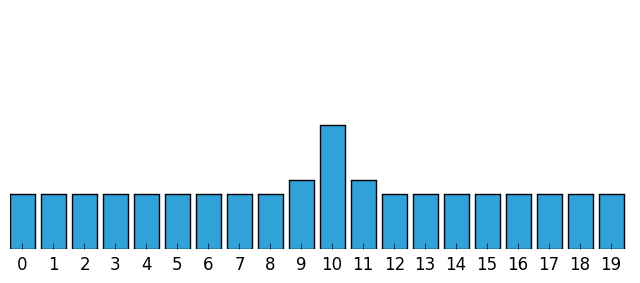
\includegraphics[scale=0.4]{./images/ex24/ex24coll10.png}
\end{subfigure}
\begin{subfigure}{\textwidth}
\centering

\includegraphics[scale=0.4]{./images/ex24/ex24wall10.png}
\caption{First collision at 10 and the resulting map}
\end{subfigure}
\end{minipage}
\begin{minipage}{0.48\textwidth}
\centering
\begin{subfigure}{\textwidth}
\centering
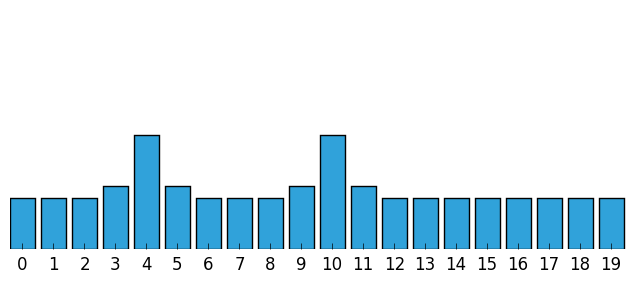
\includegraphics[scale=0.4]{./images/ex24/ex24coll4.png}
\end{subfigure}
\begin{subfigure}{\textwidth}
\centering

\includegraphics[scale=0.4]{./images/ex24/ex24wall4.png}
\caption{Next collision at 4 and the resulting map}
\end{subfigure}
\end{minipage}

\begin{minipage}{0.48\textwidth}
\centering
\begin{subfigure}{\textwidth}
\centering
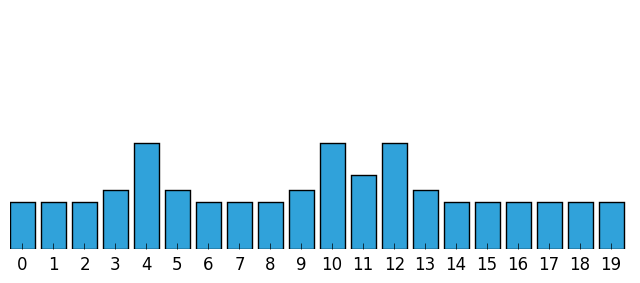
\includegraphics[scale=0.4]{./images/ex24/ex24coll12.png}
\end{subfigure}
\begin{subfigure}{\textwidth}
\centering

\includegraphics[scale=0.4]{./images/ex24/ex24wall12.png}
\caption{Next collision at 12 and the resulting map}
\end{subfigure}
\end{minipage}
\begin{minipage}{0.48\textwidth}
\centering
\begin{subfigure}{\textwidth}
\centering
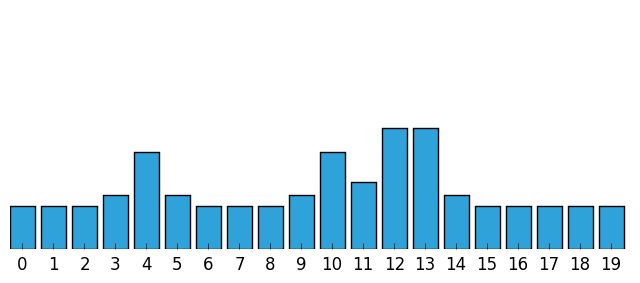
\includegraphics[scale=0.4]{./images/ex24/ex24coll13.png}
\end{subfigure}
\begin{subfigure}{\textwidth}
\centering

\includegraphics[scale=0.4]{./images/ex24/ex24wall13.png}
\caption{Next collision at 13 and the resulting map}
\end{subfigure}
\end{minipage}

\begin{minipage}{0.48\textwidth}
\centering
\begin{subfigure}{\textwidth}
\centering
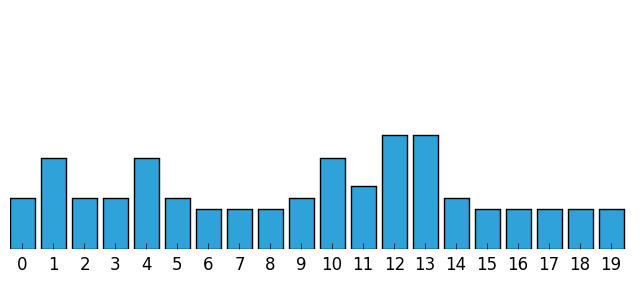
\includegraphics[scale=0.4]{./images/ex24/ex24coll1.png}
\end{subfigure}
\begin{subfigure}{\textwidth}
\centering

\includegraphics[scale=0.4]{./images/ex24/ex24wall1.png}
\caption{Next collision at 1 and the resulting map}
\end{subfigure}
\end{minipage}
\begin{minipage}{0.48\textwidth}
\centering
\begin{subfigure}{\textwidth}
\centering
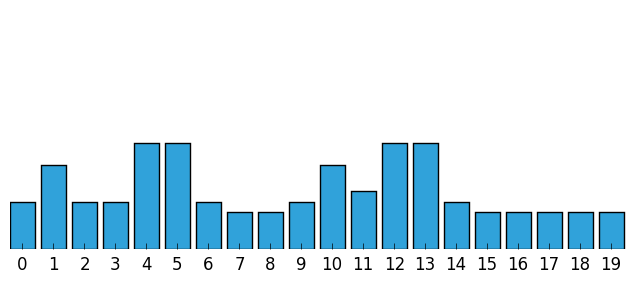
\includegraphics[scale=0.4]{./images/ex24/ex24coll5.png}
\end{subfigure}
\begin{subfigure}{\textwidth}
\centering

\includegraphics[scale=0.4]{./images/ex24/ex24wall5.png}
\caption{Next collision at 5 and the resulting map}
\end{subfigure}
\end{minipage}

\begin{minipage}{0.48\textwidth}
\centering
\begin{subfigure}{\textwidth}
\centering
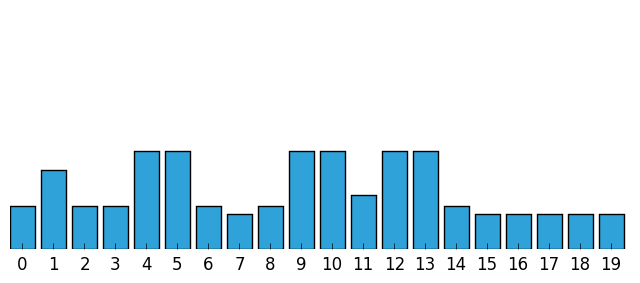
\includegraphics[scale=0.4]{./images/ex24/ex24coll9.png}
\end{subfigure}
\begin{subfigure}{\textwidth}
\centering

\includegraphics[scale=0.4]{./images/ex24/ex24wall9.png}
\caption{Next collision at 9 and the resulting map}
\end{subfigure}
\end{minipage}
\begin{minipage}{0.48\textwidth}
\centering
\begin{subfigure}{\textwidth}
\centering
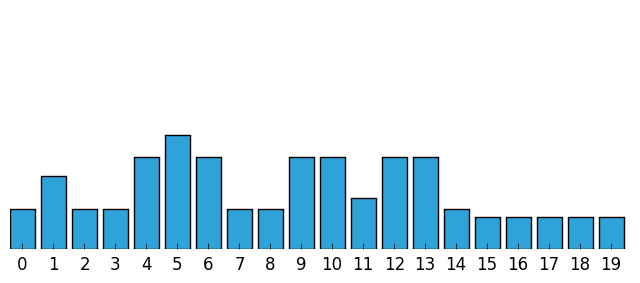
\includegraphics[scale=0.4]{./images/ex24/ex24coll6.png}
\end{subfigure}
\begin{subfigure}{\textwidth}
\centering

\includegraphics[scale=0.4]{./images/ex24/ex24wall6.png}
\caption{Next collision at 6 and the resulting map}
\end{subfigure}
\end{minipage}

\begin{minipage}{0.48\textwidth}
\centering
\begin{subfigure}{\textwidth}
\centering
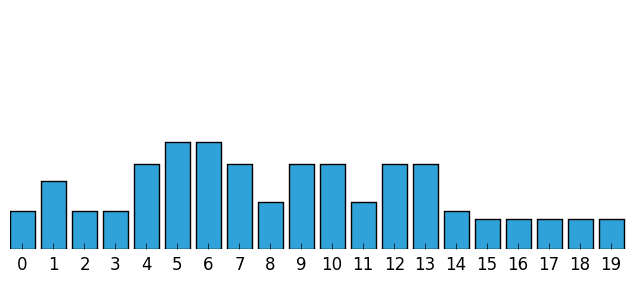
\includegraphics[scale=0.4]{./images/ex24/ex24coll7.png}
\end{subfigure}
\begin{subfigure}{\textwidth}
\centering

\includegraphics[scale=0.4]{./images/ex24/ex24wall7.png}
\caption{Next collision at 7 and the resulting map}
\end{subfigure}
\end{minipage}
\begin{minipage}{0.48\textwidth}
\centering
\begin{subfigure}{\textwidth}
\centering
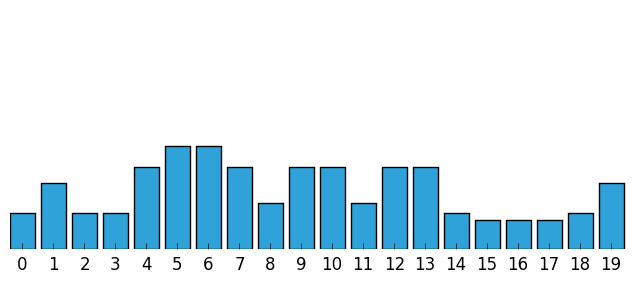
\includegraphics[scale=0.4]{./images/ex24/ex24coll19.png}
\end{subfigure}
\begin{subfigure}{\textwidth}
\centering
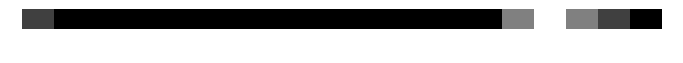
\includegraphics[scale=0.4]{./images/ex24/ex24wall19.png}
\caption{Last collision at 19 and the resulting map}
\end{subfigure}
\end{minipage}
\caption[Histogram propagation for a sequence of collision information]{Histogram propagation for a sequence of collisions}
\label{ex24_collisions}
\end{figure}

In the case the robot passes through an open door and returns back, a simple negative update is added. This update is illustrated in Figure~\ref{ex24_coll15}. \hfill $\square$
\begin{figure}
\centering
\begin{subfigure}{\textwidth}
\centering
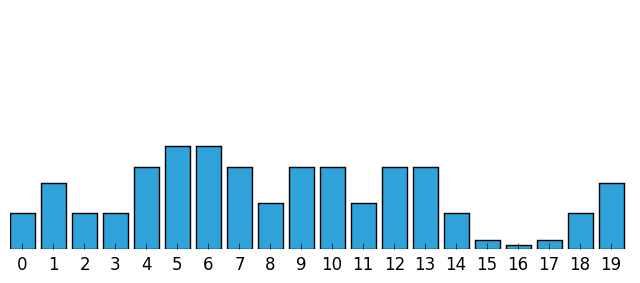
\includegraphics[scale=0.4]{./images/ex24/ex24coll15.png}
\end{subfigure}
\begin{subfigure}{\textwidth}
\centering

\includegraphics[scale=0.4]{./images/ex24/ex24wall15.png}
\end{subfigure}
\caption[Update of negative information in histogram]{Negative update of histogram at 15 and the resulting map}
\label{ex24_coll15}
\end{figure}
\label{ex24}
\end{exmp}   

\section{Challenges} \label{sec::challenges}
There are few challenges playing a key role to the success of a SLAM solution which limit the applicability based on robot sensors and mapping environment. Among the following challenges, lack of observability is a key fundamental limitation to state estimation in a generic SLAM. In a usual SLAM estimation, observability is presumed (with knowledge of few absolute locations) and hence it has to be made sure that the impact-based SLAM satisfies the observability property as well. Other crucial factors are data association, computational effort and consistency of estimates. The computational issues related to state-of-the-art SLAM estimation have been addressed in Section~\ref{sec::ekfslam} of Chapter~\ref{chap::intro}. 

\subsection{Observability}
Observability is a key property to be satisfied for any successful state estimation. SLAM is a nonlinear-coupled problem and hence simple linear analysis tools fail to explain the observability of SLAM. It is apparent from process model (Equation~\ref{proc_model}) is nonlinear and coupled. This also holds true for the odometric motion model where the nonlinear and coupled nature is introduced through the collision measurement equation (Equation~\ref{measurement_eq}). 

To determine the observability criterion for a general nonlinear coupled system, let us consider a smooth nonlinear system,
\begin{align*}
\dot{x} &= f(x)+\sum_{j=1}^m g_j(x)\cdot u_j, \hspace{1cm} u=col(u_1,\dots,u_m)\in\mathcal{R}^m\\
y_i &= h_i(x), \hspace{1cm} i\in p
\end{align*}
where $h=col(h_1,\dots,h_p):\mathcal{R}^n\rightarrow\mathcal{R}^p$ is a smooth output map or vector field of the system. 

The concept of observability is linked to \textit{indistinguishability} of a state since the effect of control inputs play a role in nonlinear observability. Before defining observability, the definition of \textit{indistinguishability} is first laid out.

\begin{rem}
Two states $x_1$ and $x_2$ are $\mathrm{V}$-distinguishable if there exists an input which drives system trajectories from both $x_1$ and $x_2$ remain in $\mathrm{V}$ such that the output functions are distinguishable $h(x_1)\neq h(x_2)$. Otherwise, the states $x_1$ and $x_2$ are $\mathrm{V}$-indistinguishable.
\end{rem}

The system is said to be locally observable if it can instantaneously distinguish a state from its neighbours. A rank condition test is used to determine the local observability of a given system, as shown below,
\begin{equation}
span(\mathcal{O}) = span(\begin{bmatrix}dh_1(x_0),\dots,dh_p(x_0),dL_{v_k}L_{v_{k-1}}\cdots L_{v_1}h_j(x_0)\end{bmatrix}) = n,
\end{equation}
where $v_i,i\in k$ is a vector field in the set $\left\lbrace f,g_1,\dots,g_m\right\rbrace$ and $L_{v_i}h_j$ is the Lie derivative of $h_j$ along the vector field $v_i$.

For a world-centric impact-based SLAM problem, the system state can be represented as,
\begin{equation}
x=\begin{bmatrix}x_r & y_r & \psi_r & x_l & y_l & \psi_l\end{bmatrix},
\end{equation} 
where first three variables represent the robot pose (position $x$ and $y$, orientation $\psi$) while the latter represents the landmark pose.

The representation included a single feature and can be generalized for observing as many features as possible. Using the process (unicycle) model,
\begin{align}
\dot{X}&=\frac{d}{dt}\begin{bmatrix}x_r & y_r & \psi_r & x_l & y_l & \psi_l\end{bmatrix}^ T \nonumber \\
&=\begin{bmatrix}\cos\psi_r & \sin\psi_r & \tan(\alpha)/L & 0 & 0 & 0 \end{bmatrix}^Tv, \label{proc_model}
\end{align}
where \lsymb{$v$}{Robot velocity control} and \gsymb{$\alpha$}{Robot heading control} represent the robot velocity and heading angle respectively. $L$ denotes the wheel base length.

For the impact-based SLAM problem, the odometry as measurement gives the position and orientation of the robot. A nice feature about impact-based SLAM is that at the instant of collision, the absolute location of landmark is the same as the absolute location of the robot. The measurement function as a result has a diagonal structure which makes the Jacobian computation and observability analysis easier.

The observation of a landmark given the robot and observed landmark pose is,
\begin{equation}
y_l = \begin{bmatrix}x_r \\ y_r \\ c_r\end{bmatrix} = \begin{bmatrix}
x_l \\ y_l \\ \tan(\psi_l-\psi_r),
\end{bmatrix}
\label{measurement_eq}
\end{equation}
where $y_l$ is the expected sensor measurement of the $l^{\text{th}}$ landmark. The measurement $c_r$ is a analytical expression obtained through the geometry of robot impact against a rectilinear wall.

By taking zero-order Lie derivatives, we can get the rank condition satisfied assuming the initial condition of the system or initial robot pose is known.
\begin{equation}
\mathcal{O}=\begin{bmatrix}
1 & 0 & 0 & 0 & 0 & 0 \\
0 & 1 & 0 & 0 & 0 & 0 \\
0 & 0 & 1 & 0 & 0 & 0 \\
0 & 0 & 0 & 1 & 0 & 0 \\
0 & 0 & 0 & 0 & 1 & 0 \\
0 & 0 & -s^2 & 0 & 0 & s^2 \\
& & \vdots & &  &
\end{bmatrix}
\end{equation}

The rank condition is satisfied with $rank(\mathcal{O})=6$. The result can be generalized for observation of as many landmarks as possible. $s^2$ represents $\sec^2(\psi_l-\psi_r)$ which is the derivative of measurement equation.

However, there is a downside to the impact based mapping for SLAM. At the instant of collision, the robot is touching the wall which makes the assumption of a smooth pose distribution invalid. The resulting pose distribution can only be represented by a set of particles which makes particle filter most suitable for localization. This is because the landmark (covariance) representation has to be consistent with the current robot pose (covariance) representation at the point of collision and this has to hold vice-versa. This fundamental representation of probability distribution must hold true for propagation of pose and landmark estimates to ensure consistency in estimation. Figure~\ref{robot_wall} illustrates the representation of probability distribution for impact-based approach to mapping.

\begin{figure}
\centering
\begin{subfigure}{0.3\textwidth}
\centering
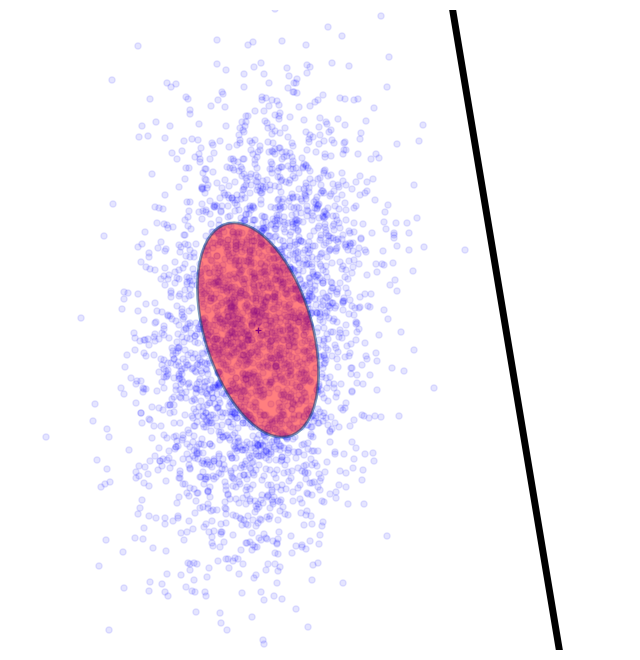
\includegraphics[scale=0.25]{./images/wall_robot.png}
\caption{}
\label{wall_robota}
\end{subfigure}
\begin{subfigure}{0.3\textwidth}
\centering
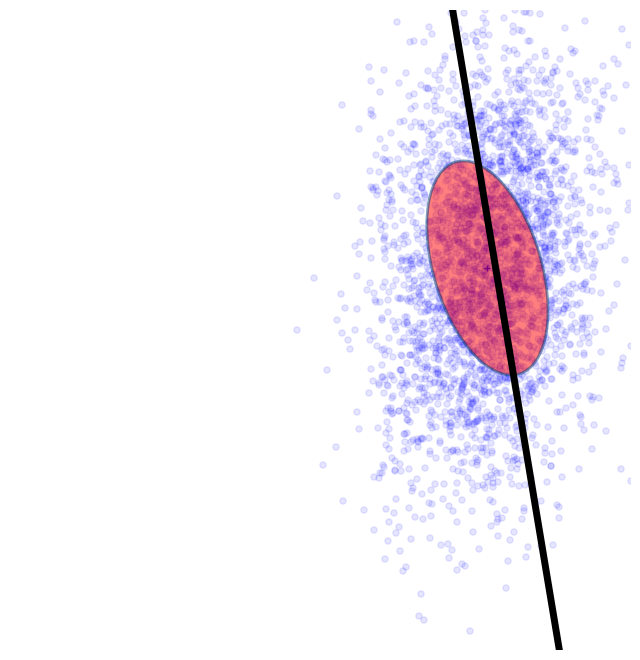
\includegraphics[scale=0.25]{./images/wall_onrobot.png}
\caption{}
\label{wall_robotb}
\end{subfigure}
\begin{subfigure}{0.3\textwidth}
\centering
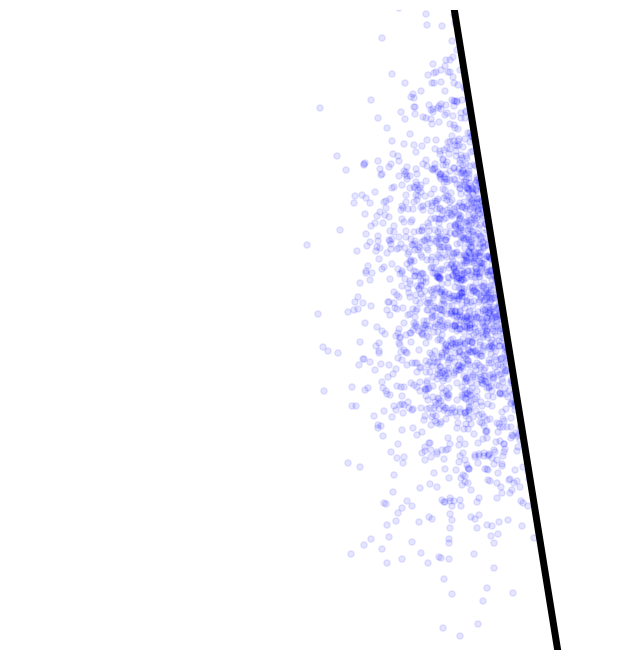
\includegraphics[scale=0.25]{./images/wall_robotp.png}
\caption{}
\label{wall_robotc}
\end{subfigure}
\caption[Gaussian and particle representation of robot pose distribution]{\subref{wall_robota} Gaussian and sampled representation of robot pose uncertainty moving towards a wall, \subref{wall_robotb} Gaussian and sampled representation of robot pose uncertainty for colliding against the wall, \subref{wall_robotc} Sampled representation of pose uncertainty taking wall constraints into account}
\label{robot_wall}
\end{figure} 

\subsection{Correlation and Consistency} \label{sec::conscorr}
The correlation through robot pose error has been considered a crucial factor in the SLAM problem since it has contributed to the tractability of the problem. However, the problem of introducing uncertainty as a bridging factor between localization and mapping has their own ups and downs. 

The main advantage, as mentioned, is the tractability in solving the SLAM problem since it can be used to improvise the robot pose estimate through reobservation of old landmarks. The robot tries to correct its pose and simultaneously improves the pose of all the previously observed landmarks due to the common correlation in the observations. The solutions dealing with explicit correlations are shown to be successful in practical implementations \cite{durrant2006simultaneous}. The representation of correlations through uncertainty information has led to the popularity of the probabilistic methods in SLAM.      

However, there is a downside to the use of robot uncertainty (process noise) in the problem as the bridging factor. The effect of using uncertainty to influence the observability in the problem has a dig at the consistency of the estimation. To improve the convergence of the solution to the problem, the correlation have to improve with time, or said in other words, higher the correlation, better is the SLAM. The problem is that increase in uncertainty, if not properly modelled in SLAM, can be really problematic since it can lead to optimistic estimates of the uncertain state variables which cannot be compensated unlike in usual tracking and navigation problems.  

Before getting into the problems of consistency due to the structure and assumptions in SLAM, the definition \cite{julier2001counter} is first laid out.
\begin{defn}
An estimator is said to be consistent if the estimated state converges to the true value and remains thereon unless an external disturbance acts on it. If $e_n$ is the error in the estimate, the true covariance or variation in the actual system state can be written as $E(e_n^Te_n)$. $\Sigma_n$ is the estimated covariance or estimated variation of error in the system. 

Mathematically, an unbiased estimator is consistent if and only if it can capture the true variation in error. 
\begin{equation}
\Sigma_n=E(e_n^Te_n)
\end{equation} 
\end{defn}

However, this condition of consistency is difficult to establish due to the stochastic scenario of a system. To enforce consistency, conservativeness is introduced so that we can bound the true variation of error at all time instances. Mathematically,
\begin{equation}
\Sigma_n-E(e_n^Te_n)\geq 0
\end{equation} 

A standard solution to ensure consistency is to inflate the observation covariance by padding it with sufficiently large values. This process is called as ``covariance inflation'' or injection of stabilizing noise into the system \cite{julier2003stability}. There is however a problem associated with this technique. Due to the inflation of noise covariance, the assumed uncertainties in certain directions of state space increases and as a result, the steady state covariance can grow unbounded.

Consistency in the SLAM scenario can be discussed based on the estimator or optimization technique to be implemented for the SLAM problem. The question of consistency can raise from several issues related to the SLAM problem such as data association errors, modelling errors, transformation errors.

The effect of data association is highly sensitive and a single incorrect association will lead to inconsistency in the solution. The first issue has been addressed a lot in the literature \cite{cooper2005comparison} and is detailed for the impact-based SLAM problem in the next section. The effect of inconsistency due to probability transformation errors have been studied and suitable solutions are developed in \cite{julier2004unscented}. The inconsistency issues relevant to EKF-SLAM and particle filter-SLAM are discussed below.

\subsubsection{EKF-SLAM}
The structure and properties of the Extended Kalman Filter-SLAM, as discussed previously, will be revisited to discuss about source and effects of inconsistency. The inconsistency in EKF-SLAM arises from linearization error in observation and inverse observation models.

To ensure consistency, the following condition \cite{julier2001counter} has to be satisfied,
\begin{equation}
\nabla h_s - \nabla h_{m_i}\nabla g_s = 0
\end{equation}
where $\nabla h_s$, $\nabla h_{m_i}$ represent the Jacobian of the measurement function with respect to robot state and landmark estimate respectively. $\nabla g_s$ denotes the Jacobian of inverse measurement function with respect to the state. Usually, this function is never satisfied due to linearization errors and as a result, the estimates turn inconsistent. As the relationship depends upon the nonlinear system models and noisy state estimates, the linearization error is difficult to compute and cannot be compensated through inflation of error covariance. 

The effect of linearization errors can be reduced through local map fusion which uses the robot's local coordinate frame to update the map \cite{castellanos2007robocentric}. This approach has a lower error in the state estimates which in turn reduces the effect of inconsistency. The use of multiple robots in impact-based SLAM ensures a higher consistency in the local map updates which can be later merged. Other approaches such as observability constrained estimation \cite{huang2011observability} also ensures a more consistent state estimation at every time step.

\subsubsection{Particle filter-SLAM}
An advantage about the use of particle filters is elimination of inconsistency due to probability transformation errors since the particle set can be propagated through any nonlinear model. 

However, there are two other key issues related to inconsistency in particle filter-SLAM. The first issue is inconsistency through modelling errors and the second i degeneracy in the estimation process.

The particle filter-SLAM problem exploits the Rao-Blackwellized property where landmark estimation problems are conditional independent given the robot trajectory. This property is based on on the assumption that the environment is unstructured, or in other words, the environment contains randomly placed landmarks. The only correlation factor is the robot pose error in the SLAM problem which is conditioned to make the landmark estimation independent. However, in the case of a rectilinear environment, the landmarks are correlated through the geometric symmetry in the environment such as orthogonal walls. Hence, a straightforward implementation of Rao-Blackwellized particle filter to SLAM problem results in inconsistent estimation. 

The effect of cross-correlations cannot be ignored since they are crucial for ensuring consistency in the SLAM estimation. The lack of proper correlations leads to a poor covariance estimate which leads to inconsistency (refer Remark~\ref{rem_corr}). The cross-correlations in the environment can be effectively maintained using a joint covariance matrix (a single EKF for all the landmarks) for every particle in the particle set. This approach might lead to computational issues since every measurement update requires a computation complexity of $\mathcal{O}(M\cdot N^2)$ which is cumbersome.

A more computationally efficient approach is to conservatively incorporate the conditionally independent landmarks (through Rao-Blackwellization) with the orthogonality and partial uncertainty constraints through \acf{CI} technique \cite{julier2007using}. This approach ensures a consistent estimation in a conservative fashion at the expense of optimal performance (rate of map convergence). With this approach, the computational efficiency of Rao-Blackwellization is still maintained.

For the case of degeneracy, the particle filter-SLAM produces optimistic uncertain estimates in the long term, \cite{bailey2006consistency}. In general, particle filters provide a consistent recursive estimation through resampling in situations where a system exponentially forgets its past estimate errors. The problem in particle filter-SLAM is that the past pose errors are never forgotten since they are recorded in the map estimates through correlations and each time a resampling is performed, the particle that is not selected gets thrown out with an entire map hypothesis. Hence, the particle filter degenerates a good knowledge of map hypotheses and the most likely particle (with largest importance weight) duplicates by replacing other unlikely particles in the resampling step. 

As a result, there is a variance reduction in the particle set which can result in an underestimated covariance. The algorithm starts to get optimistic about the uncertainty in the trajectory of the robot and the landmark locations. Every time a particle is lost due to resampling, an entire map hypothesis is lost and there is a depletion of historical information. Hence, the overall map statistics degrade and the algorithm finds it difficult to close larger loops. Moreover with the loss of past information, data association errors cannot be corrected based on the future measurements which brings brittleness in data association similar to standard EKF-SLAM.

In the short term, particle filter-SLAM might produce consistent results given a sufficient number of particles. To avoid this problem, adaptive resampling techniques are adopted to ensure long term consistency in the solution. In addition, impact-based SLAM have sparse measurements with frequent loop closures (in corridors) which might result in degeneracy. This can be avoided through the inclusion of measurements in the prediction step, resulting in a more consistent estimate with less number of particles. Section~\ref{sec::fastslam_pred}~and~\ref{sec::fastslam_resample} detail the modified prediction step and and adaptive resampling techniques for the impact-based SLAM problem.

\subsection{Data Association} \label{sec::da}
Data association determines the mapping from the measurements to the landmarks and it is one among the essentials for achieving a successful SLAM solution. The association is quite sensitive to the uncertainty of robot involved in SLAM and few incorrect associations can lead to inconsistency in the SLAM estimation. Over the past years, this issue has been dealt seriously and robust data association techniques were developed to ensure consistency.

The data association algorithm depends upon the characteristics of landmarks and availability of measurements. Two of the most popular approaches for data association are \acf{ML} and \acf{JCBB} \cite{bailey2006simultaneous}, former being the simplest and vulnerable one.  The later approach is most useful for a SLAM where batch measurements are available for processing at each time instant. Apart from the two approaches, Multiple Hypotheses data association \cite{jensfelt2001active} has been the most accurate of all but with a computational burden of maintaining all the possible associations of landmarks with measurements.  

For impact-based SLAM using particle filter, each particle maintains a copy of the map and hence, data association decisions can be made on a per-particle basis. This leads to a robust multiple hypothesis association. The particles are not only a representation of uncertainty of state estimate but are also individual hypothesis of the map. Hence, Multiple Hypotheses is ingrained in the particle filter-SLAM formulation.

Among the data association algorithms, the most suitable one is \acf{ML} association where each particle performs a ML association for the incoming measurements. 

\begin{rem}
In data association, following assumptions have to be considered for an analytical representation of landmark likelihood to a measurement.
\begin{enumerate}
\item The incoming measurements are normally distributed, i.e., the measurement noise is Gaussian
\item Knowledge of the Gaussian parameters, mean and standard deviation, are available a-priori 
\end{enumerate}
\end{rem}

The data association is computed using likelihood function, also known as $\chi^2$ test. The maximum likelihood problem is posed as shown below,
\begin{equation}
d_l = \arg\max_{j}\frac{1}{\left(2\pi\right)^{n/2}\cdot\sqrt{\strut S_j}}\exp\left(-\frac{1}{2}e_{ij}^T\cdot S_j^{-1}\cdot e_{ij}\right),
\label{da_pfslam}
\end{equation}
where $d_l$ is the $l^{\text{th}}$ data association for measurement $i$ and landmark $j$. The variable $e_{ij}$ is the innovation vector for the pair $\left\lbrace i,j\right\rbrace$ pair, $S_j$ is the innovation covariance matrix and $n$ is defined as the dimension of the innovation vector.

\begin{rem}
The solution can also be computed through log-likelihood for numerical stability. This approach is more suitable for data associations over multiple measurements or smoothing process in the estimation process.
\end{rem}

In the case of multiple measurements or smoothing process, the measurements are considered as a vector and are assumed to be independent. Hence, the likelihood is defined as joint probability, which under the measurement independence assumption, factor into a product of marginal probabilities and the magnitude of the likelihood can be quite small, often very close to zero. With a large number of observations, this value can approach the machine zero of the computing device used, leading to numerical problems. Log-transforming all these probabilities will convert these small numbers into negative numbers thus eliminating numerical instability. The solution however still remains to be the same due to the increase monotonicity of the log-function.

Taking logarithm over the likelihood, the problem is rewritten as shown below.
\begin{equation}
d_l = \arg\max_{j}\left(-\frac{1}{2}e_{ij}^T\cdot S_j^{-1}\cdot e_{ij}+\ln\left(\frac{1}{\left(2\pi\right)^{n/2}\cdot\sqrt{\strut S_j}}\right)\right)
\end{equation}

An equivalent normalized-minimization problem can also be posed as follows,
\begin{equation}
d_l = \arg\min_{j}\left(e_{ij}^T\cdot S_j^{-1}\cdot e_{ij}+\ln(|S_j|)\right).
\end{equation}

\textbf{Summary} 
In this chapter, a probabilistic formulation of the impact-based SLAM problem is laid out from the perspective of online estimation. Two robot motion models are described using a unicycle model framework for the SLAM problem. Suitable environment representations are studied for the impact-based SLAM along with the proposed histogram map. Various challenges such as observability, correlations, consistency and data association are addressed from the viewpoint of impact-based SLAM.
\chapter{SLAM solution}  \label{chap::solution}
{\it \centering This chapter focusses exclusively on the solution to the impact-based SLAM problem. A modified version of the particle filter-SLAM algorithm will be developed to suit rectilinear environments, and the problem is extended to multiple robots for map-merging. Simulation results support the developed algorithm for both single robot and multiple robot-SLAM.}

\section{Factored representation} \label{sec::factpf}
In particle filter-SLAM, the uncertainty of robot pose is represented by a particle set (see Figure~\ref{robot_wall}) rather than a smooth parametric Gaussian as in EKF-SLAM. This representation has great advantages of representing any arbitrary multi-modal distribution, and they can be easily propagated through any probabilistic robot motion models.

However, there are downsides to implementing particle filter for SLAM due to a key reason. The number of particles scales exponentially with the dimension of the state space which restrict the use of particle filters to low-dimensional estimation and tracking problems. A suitable representation of particle filter towards the SLAM problem would be essential for an accurate SLAM solution. As discussed in Section~\ref{sec::pfslam}, the conditional independence property of the mapping problem given the robot trajectory is a key structure which can be exploited. This structural property in SLAM or any probabilistic problem that factorizes a joint distribution to conditional distributions is \textit{Rao-Blackwellization}.

Appendix~\ref{chap::rbpf} will provide a detailed proof of the conditional independence property in SLAM posterior and the exact nature of the factorization. Under this structure, cross-correlations between the landmarks introduced by the robot path uncertainty need not be maintained, and in the case of structured environments, explicit constraints are incorporated through \acs{CI} technique for ensuring consistency in estimation. The SLAM algorithms in future will utilize the conditional independence property for efficient computation of the posterior.

\section{Particle filter-SLAM}

Using the factored representation of the SLAM posterior, the SLAM solution can be obtained with linear time complexity in the number of landmarks, and the accuracy of obtained solution is proportional to the size of the particles. The particle filter-SLAM algorithm is simple and intuitive and a detailed algorithm is provided at each and every step.

Before delving into an algorithm, inclusion of data association into the SLAM posterior has to be discussed. The previous examples and illustrations assumed that data association is known, which is not the usual in SLAM. The general SLAM posterior is,
\begin{equation}
p(s_{1:t},m,c_{1:t}|z_{1:t},u_{1:t}),
\end{equation}  
where the it can be factorized through Bayes' product rule,
\begin{equation}
p(s_{1:t},m,c_{1:t}|z_{1:t},u_{1:t}) = p(s_{1:t},m|z_{1:t},u_{1:t},c_{1:t})\cdot p(c_{1:t}|z_{1:t},u_{1:t}).
\label{eq_slprod}
\end{equation}

The first term of the product is same as the old SLAM posterior and the second term correspond to the data association conditioned upon the observations. The vector $c_{1:t}$ is a vector of correspondences where each component makes a correspondence between a feature and a measurement.

\begin{rem}
The second term of the product in Equation~\ref{eq_slprod} corresponds to the data association, conditioned on the observations but not on the robot path. This discrete prior distribution about landmarks is not available initially and has to be engineered according to the sensors and operating environment.
\end{rem}

The FastSLAM algorithm maintains the (first term of the product) posterior distribution as a set of samples where each particle in the sample set corresponds to the state vector. According to the conditioned distribution, the map has to be conditioned on the robot trajectory and the length of each particle will grow over time. However, the update equations in FastSLAM, as in Section \ref{sec::pfslam}, do not depend upon the entire trajectory but only upon the most recent pose. Hence, each particle needs to contain the most recent pose and a map of the environment.

Each particle in the particle set $Y_t=\left\lbrace Y_t^{[1]}, Y_t^{[2]}, \dots, Y_t^{[M]}\right\rbrace$ of size $M$ takes the form as in Equation~\ref{psf},
\begin{equation}
Y_t^{[k]}=\left\langle s_t^{[k]}, \mu_{1,t}^{[k]}, \Sigma_{1,t}^{[k]}, \dots, \mu_{N,t}^{[k]}, \Sigma_{N,t}^{[k]} \right\rangle
\end{equation}  

The $k^{\text{th}}$ particle contains the recent robot pose and a corresponding set of landmarks of size $N$ where landmark $i$ is described by mean $\mu_{i,t}^{[k]}$ and covariance $\Sigma_{i,t}^{[k]}$ at time $t$.

From the particle set, the particles are propagated or sampled from the probabilistic motion model and the corresponding step is called as the Prediction step. The particles are then updated using incoming set of measurements and resampled if necessary. A simple flowchart explaining the process involved in the FastSLAM algorithm is illustrated in Figure \ref{flow_fs}. 
\begin{figure}
\centering
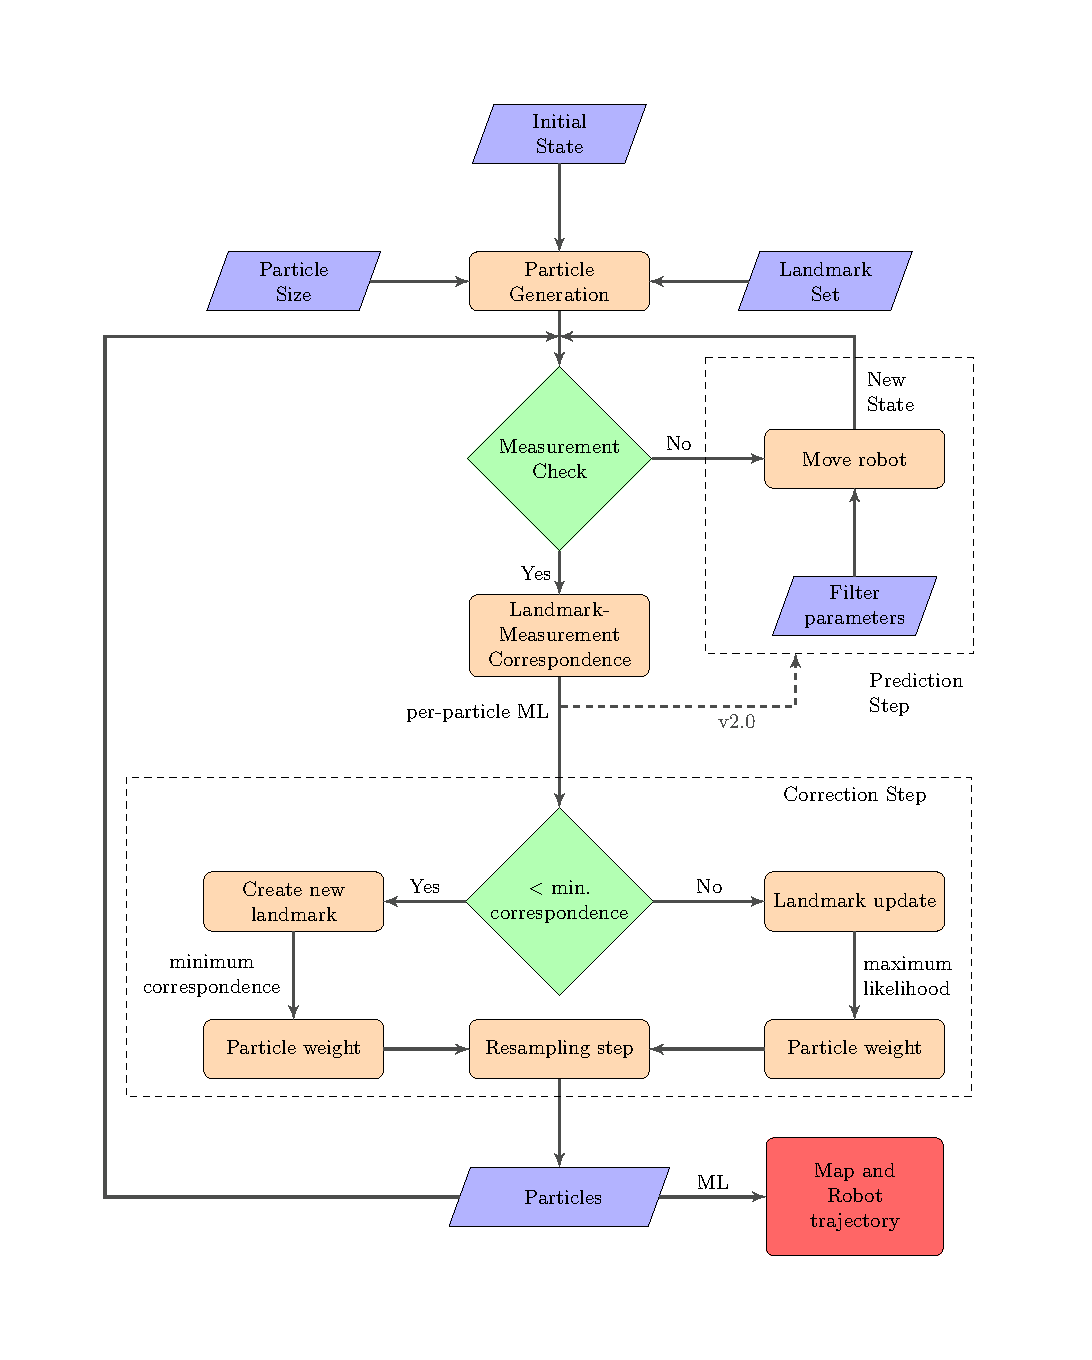
\includegraphics[scale=0.9]{./images/flow_fs}
\caption[A flowchart of particle filter-SLAM algorithm]{Particle filter-SLAM algorithm}
\label{flow_fs}
\end{figure}

The following sections will detail the individual steps involved in the algorithm.

\subsection{Particle generation}
Initially, a particle set of given size has to be created from a known distribution. The particles are either sampled from a Gaussian distribution whose mean correspond to the initial state of the robot and covariance corresponding the pose error or they are sampled from a prior particle distribution. In the SLAM scenario, the initial uncertainty is taken to be zero with no prior knowledge of landmarks.
\begin{equation}
Y_t^{[k]}=\left\langle s_0 \right\rangle
\end{equation}

As all the particles have the same initial state, the individual maps will also have the origin as the initial state.

\begin{rem}
The initial uncertainty in the position estimates (both robot and landmark) can also be non-zero, which ultimately converges to a stable solution. This can improve the initial diversity of the estimates and thereby ensuring a more consistent solution at the expense of time to converge to an accurate map. 
\end{rem}

\subsection{Prediction step} \label{sec::fastslam_pred}
The new state estimate is sampled from the old state using the probabilistic motion model and controls. The two motion models suitable to the SLAM scenario, along with the algorithm, are detailed in Section~\ref{sec::robotmodel}. 

The propagation of particles through the motion model has a linear time complexity $\mathcal{O}(M)$ and the new state estimate from each particle constitute to form a temporary particle set called as proposal distribution. This distribution takes the following form asymptotically,
\begin{equation}
p(s_t|u_t,s_{t-1})
\end{equation}

As the measurement likelihood is sparse or discrete with respect to the pose space in impact-based SLAM, the SLAM solution can be approximated to a Gaussian using Markov assumption for the measurement model. The current measurement depends upon the current robot pose and not on the previous set of poses. This assumption holds valid only since a complete state (refer Definition~\ref{def1}) is defined for the impact-based SLAM problem. Hence, the prediction step has to be repeated till a measurement is made available. The robot moves between the walls and a measurement is available only during a wall collision. As a result, the uncertainty in robot pose increases till a measurement is available.

The resulting motion model can be quite noisy and as said in the previous Chapter, this might result in a degeneracy problem. This arises when the robot motion is more noisy than the measurements. In the case of impact-based SLAM, the motion noise gets accumulated till a single measurement is made. Less particles will now be able to explain the new measurement and hence, particle diversity and consistency are lost during resampling(see Section~\ref{sec::conscorr} for more details). 

A favourable solution to the degeneracy problem is to modify the prediction step to include the measurements such that the proposal distribution is generated in accordance to incoming measurements \cite{montemerlo2007fastslam}. The modified proposal distribution can be written as,
\begin{equation}
p(s_t|s^{[k]}_{t-1},u_{1:t},z_{1:t},c_{1:t})
\end{equation}

In short, the variance propagation of measurements get included into the prediction step to obtain a better proposal distribution that can explain the incoming measurement. Hence, the proposal distribution remains closely same as the posterior distribution and particle diversity is retained. Appendix~\ref{mod_prop} gives a detailed proof of the modified proposal distribution.

For impact-based SLAM, the robot changes its heading direction (orientation in yaw axis) after every collision, which is encoded through a \acf{FSM} as shown in Figure~\ref{fsm4}. The FSM is modelled taking into account the exact nature of motion of robot between collisions. In forward motion, the robot can collide with the wall either on the left side or on the right side as shown in Figure~\ref{collision_ball}. This can restrict the size of FSM to two translational motion states (red shaded nodes) as in Figure~\ref{fsm4} where the left side represents the heading of robot towards a wall from left side and the other from right side. The rotation states describe the change in robot's orientation after every collision.

\begin{figure}
\centering
\includegraphics[scale=0.75]{./images/fsm4}
\caption[Finite State Machine model of robot-wall collisions]{Finite State Machine model of the robot motion between collisions. The red shaded nodes indicate the motion model of the robot. The gray and white shaded nodes indicate a specific control action on orientation corresponding to the sign of $a_x$. $\theta_d$ indicates the final desired angle through the function $T_i(\cdot)$ as in Equations~\ref{t1_orientation}~and~\ref{t2_orientation}.}
\label{fsm4}
\end{figure}

\begin{figure}
\centering
\includegraphics[scale=0.6]{./images/collision_ball}
\caption[Types of collision generation in impact-based SLAM]{Approach of robot towards a rectilinear wall restricts to two possible cases, left-handed collision and right-handed collision. The black arrows depict the local coordinate frame of the robot before collision and the red arrows depicts the robot motion. The ratio of change in impact force along the individual axis is used as collision measurement.}
\label{collision_ball}
\end{figure}

The underlying motion model used for the FSM in prediction step is the same unicycle model in Section~\ref{sec::robotmodel} as follows,
\begin{equation}
s'\sim p(s_t|s_{t-1},u_t)
\end{equation}

The change in robot's orientation depends upon the collision of the robot with the wall from the left or right hand side. With a coordinate frame is assigned to the robot, the forward motion of the robot is Y-axis and to the right is X-axis. As the collision detection is achieved through changes in the accelerometer values, the left-handed collision of the robot with a wall has negative acceleration on the X-axis while the right-handed collision of the robot with a wall has positive acceleration on the X-axis. This can be described through a change in orientation for the robot where the left-handed collision model is written as,
\begin{equation}
T_1(\theta,a_x)=\theta-\left(\pi-c\cdot\arctan\left(\frac{a_x}{a_y}\right)\right),
\label{t1_orientation}
\end{equation}
and the right-handed collision model as,
\begin{equation}
T_2(\theta,a_x)=\theta+\left(\pi-c\cdot\arctan\left(\frac{a_x}{a_y}\right)\right).
\label{t2_orientation}
\end{equation}

The constant $c$ is the reflection constant which varies according to the requirement of desired heading after a collision. For a reflective collision i.e., angle of incidence is same as angle of reflection, the value of $c$ is 2. The initial orientation $\theta$ in yaw axis of the robot is obtained from the IMU. Further details of Sphero robot motion after collision is detailed in Section~\ref{sec::single_slam}.  

\begin{rem}
The false positives in collision detection may arise from the positive acceleration in the forward direction. This can be avoided by considering only the positive acceleration hyperplane in collision detection, i.e., $a_y>0$.
\end{rem}

\subsection{Data Association}
The data association for the impact-based SLAM performs a landmark-measurement likelihood computation on a per-particle basis. Three key advantages with the per-particle data association are as follows,
\begin{itemize}
\item Multi-hypothesis data association is the robust form of data association till date.
\item Consistent landmark updates can be carried out on a per-particle basis since landmarks in a particle do not depend upon robot pose uncertainty as robot pose error is factored out.
\item Data association decisions can be revisited by removing particles which cannot explain incoming measurements and resampled with a particle which is consistent with new measurements. 
\end{itemize}

The association is sensitive to the source of uncertainty arising from the motion or measurement model. An increase in measurement noise can lead to a wrong association of a measurement to a landmark. This is because as the measurement uncertainty increases, the distribution of measurements from nearby landmarks start to substantially overlap. As a result, some landmarks get wrongly associated which might lead to a underestimation (spurious reduction) of covariance. This problem will have a minor impact on the SLAM solution, provided landmarks are not close by. However, the noise from the motion model will have a more drastic impact since higher uncertainty in the robot pose leads to a wide distribution of particles and the resulting per-particle data association will be quite different. This situation occurs in the impact-based SLAM problem where the motion noise gets accumulated between the sparse measurements. This problem in association can be reduced using the modified proposal distribution as mentioned in the previous section. 

Using the per-particle data association, the worst-case computational complexity involved in computing the likelihood is proportional to $\mathcal{O}(N\cdot n^3)$, where $N$ is the size of landmark set and $n$ is the dimension of output vector. This can be computationally intensive which can be reduced on an average case through a pruning process. The process prunes the landmark with orientations which are not in the field of view for the robot, which also contributes to finite nature of FSM in a rectilinear environment. In addition, geometric constraints can be added to improve the efficiency of association. One such geometric constraint is the feature pose of the same landmark. In the robot's view, feature orientation of 0~degree always come to the right of a feature with an orientation of 180~degrees with respect to the robot's frame.   
 
\begin{figure}
\begin{algorithm}[H]
\caption{Per-particle data association} \label{ppda}
\begin{algorithmic}[1]
\BState \textbf{Input}: $z_t$, $R_t$ , $Y_t$ and $m_{1:N}$
\For{each particle \Pisymbol{psy}{206} $Y_t$}
\State $l \gets \left[\,\right]$
\For{each landmark \Pisymbol{psy}{206} $m_{1:N}$}
\State compute expected measurement
\If {geometric constraint not satisfied} 
\State $l$.append(0)
\EndIf
\If {landmark in robot's view}
\State compute likelihood
\State $l$.append(likelihood)
\ElsIf {check similar features}
\State create feature if not present in landmark list
\State compute likelihood
\State $l$.append(likelihood)
\Else 
\State $l$.append(0)
\EndIf
\EndFor
\State \Return correspondence $\gets \text{max}(l)$
\EndFor
\end{algorithmic}
\end{algorithm}
\caption[Per-particle data association algorithm]{Per-particle data association is carried out using an incoming measurement $z_t$, measurement covariance $R_t$, particle set $Y_t$ and landmark set $m_{1:N}$.}
\end{figure}

In computing the measurement likelihood, correspondence was computed only from the set of point landmarks, and histogram information is not used. Similar to occupancy maps, histogram maps can be used for localizing the robot using the occupancy information. However, a sufficient amount of collision information along the wall is necessary to influence the localization. The use of histogram information (as a probability distribution) in data association will be more promising in situations where the rectilinear landmarks are more randomly placed.  

\subsection{Landmark update} \label{sec::land_update}
The data association step might provides a landmark identity once its correspondence with a measurement satisfies the compatibility test and it is found to be more likely than other landmarks. As the data association step is carried out on a per-particle basis, the corresponding landmark update is also carried similarly. The rest of the landmark set remain unchanged.

The landmark update stage is a part of the mapping problem, described through the posterior $p(m_l|s_t,u_{1:t},z_{1:t},c_{1:t})$. Expanding the term using Bayes' product,
\begin{equation}
p(m_l|s_t,u_{1:t},z_{1:t},c_{1:t})=\eta\,p(z_t|m_l,s_t,u_{1:t},z_{1:t-1},c_{1:t})\cdot p(m_l|s_t,u_{1:t},z_{1:t-1},c_{1:t}) 
\end{equation}

The first probabilistic term of the above product corresponds to the measurement model and is approximated as a Gaussian using EKF linearization. The second term is the landmark estimate conditioned on the particle pose which is equal to the mean and covariance estimates of the landmark maintained by a particle $\mathcal{N}\left(\mu^{[k]}_{l,t-1},\Sigma^{[k]}_{l,t-1}\right)$.
 
EKF uses a linear approximation of the measurement model $h(\cdot)$ which is obtained through a first order Taylor series expansion. According to the conditioned measurement distribution, each landmark update in a particle is carried out over a fixed robot pose. This property favours computation since the Jacobian over robot pose \lsymb{$G_{s^{[k]}_t}$}{Jacobian of measurement model over particle pose} in an EKF update is unnecessary. As a result, the Jacobian over the associated landmark \lsymb{$G_{m_{l,t}}$}{Jacobian of measurement model over landmark pose} is only calculated in the Taylor expansion. 
\begin{align}
\hat{z}_t &= h(s_t^{[k]},\mu^{[k]}_{l,t-1}) \\
G_{m_{l,t}} &= \nabla_{m_l} h(s_t=s_t^{[k]},m_l=\mu^{[k]}_{l,t-1}) \\
h(s_t,m_{l,t}) &\approx \hat{z}_t+G_{m_l}(m_{l,t}-\mu^{[k]}_{l,t-1})
\label{taylor_approx}
\end{align}

The mean of the Gaussian is approximated till the first order Taylor expansion and the covariance is assumed to be known initially. The derivative of the measurement function is defined everywhere except in cases where robot and wall orientation are the same (robot collides parallel to the wall) at the point of collision. This situation is not possible in impact-based SLAM using Sphero. The parametrization of a Gaussian measurement can be written as,
\begin{equation}
\mathcal{N}(\hat{z}_t+G_{m_l}(m_l-\mu^{[k]}_{l,t}),R_t)
\end{equation}

The mean and covariance of the associated landmark can now be computed using the standard EKF update equations.
\begin{align}
S_{l,t} &= G_{m_l}\Sigma^{[k]}_{m_{l,t-1}}G^T_{m_l}+R_t \label{ekf_update1}\\ 
K_t &= \Sigma_{m_{l,t-1}}G^T_{m_{l,t}}S^{-1}_{l,t} \\
\mu^{[k]}_{l,t} &= \mu^{[k]}_{l,t-1} + K_t\left(z_t-\hat{z}_t\right) \\
\Sigma^{[k]}_{l,t} &= \left(I-K_tG_{m_l}\right)\Sigma^{[k]}_{l,t-1} \label{ekf_update2}
\end{align}

The term \lsymb{$S_{l,t}$}{Innovation covariance} and $K_t$ represent the innovation covariance of landmark $l$ and Kalman gain at time $t$ respectively.

\subsubsection{Negative evidence}
A new histogram is created once a new landmark is detected. This histogram is maintained either as a probability distribution or as a simple histogram for encoding the collision information. In the case of a probability distribution, the histogram is defined as a uniform distribution, based on the prior assumption that the distribution of mass information is unknown. The probability mass propagates into the regions where collisions were detected and a multimodal distribution is generated as seen in Figure~\ref{ex24coll_10}.

With the histogram representation, negative information can be incorporated into the map. As the robot passes through the histogram axis in the map, a negative Gaussian information is added to the histogram as shown in Figure~\ref{ex24_coll15}. This information helps in pruning the histogram support. If the environment size is known prior, the histogram support can be made finite according to the environment size.

\subsection{Landmark initialization}
The landmark is initialized each time a new measurement is unable to explain all the landmarks in the landmark set or when the landmark set is empty. The data association step in the previous section assumed that all the landmarks were available prior.

The landmarks are initialized using the inverse measurement model, provided the measurement function (see Equation~\ref{measurement_eq}) is invertible. The inverse is ill-defined in a SLAM problem when a given measurement is unable to constrain the landmark state and multiple measurements are required (as in range-only or bearing-only SLAM). However, the measurement model of impact-based SLAM is invertible since the landmark pose at time $t$ is calculated through the conditioned robot pose, odometry and collision information at time $t$.
\begin{equation}
\mu^{[k]}_{l,t}=\begin{bmatrix}x_l \\ y_l \\ \psi_l
\end{bmatrix} = \begin{bmatrix}x^{[k]}_r \\ y^{[k]}_r \\ \psi^{[k]}_r+\arctan\left(\dfrac{a_x}{a_y}\right)\end{bmatrix}
\label{inv_measurement}
\end{equation}

The landmark pose $m_l$ is described as a vector of landmark position \lsymb{$(x_l,y_l)$}{XY-position of landmark} and orientation \gsymb{$\psi_l$}{Orientation of landmark}. Similarly, the robot pose for a particle $k$ is described as a vector of robot position \lsymb{$(x^{[k]}_r,y^{[k]}_r)$}{XY- position of $k^{\text{th}}$ particle pose} and orientation \gsymb{$\psi^{[k]}_r$}{Orientation of particle pose}. \lsymb{$a_x$}{Rate of acceleration along the X axis} and \lsymb{$a_y$}{Rate of acceleration along the Y axis} denote the rate of change in accelerometer data along the X and Y axes respectively.
\begin{rem}
The offset between the position of landmark and robot at the instant of collision varies by a constant factor. This factor should be taken into account for the resulting output map of SLAM. 
\end{rem}

As the measurement is obtained from a nonlinear model, a first order Taylor expansion (as in Equation~\ref{taylor_approx}) can reveal the Gaussian nature of the noise where the difference in the approximation is the error $e_t$,
\begin{equation}
e_t=z_t-\hat{z}_t-G_{m_l}(m_l-\mu^{[k]}_{l,t})
\end{equation}
and the Gaussian as,
\begin{equation}
\mathcal{N}:= \dfrac{\displaystyle 1}{\displaystyle \sqrt{\mathstrut|2\pi R_t|}}\exp\left(-\frac{1}{2}e_t^TR_t^{-1}e_t\right)
\label{exp_gaussian}
\end{equation}

The landmark covariance is obtained through the covariance bound of the $\chi^2$ distribution (see Definition~\ref{chi2_dis}). The measurement covariance propagation through the SLAM state space is obtained by projecting the measurement covariance into the landmark state space, which is equivalent to calculating the second differential of Equation~\ref{chi2_eq}. As the landmark is defined using inverse of the measurement model, the landmark covariance is the inverse of the measurement covariance propagation.

\begin{defn}
The $\chi^2$ distribution is the negative exponent of the Gaussian $\mathcal{N}$ as shown below,
\begin{equation}
\chi^2 := \left(z_t-\hat{z}_t-G_{m_l}(m_l-\mu^{[k]}_{l,t})\right)^TR_t^{-1}\left(z_t-\hat{z}_t-G_{m_l}(m_l-\mu^{[k]}_{l,t})\right).
\label{chi2_eq}
\end{equation}
\label{chi2_dis}
\end{defn}

As a result, the mean $\mu^{[k]}_{l,t}$ is obtained through the inverse of measurement model (Equation~\ref{inv_measurement}) and the covariance $\Sigma^{[k]}_{l,t}$ is obtained from the second differential of the Equation~\ref{chi2_eq} and taking the inverse since an invertible measurement is used to define a new landmark.

\begin{align}
\mu^{[k]}_{l,t} &= h^{-1}\left(s^{[k]}_t,z_t\right) \label{landmark_init1}\\
\Sigma^{[k]}_{l,t} &= \left(G_{m_l}^TR_t^{-1}G_{m_l}\right)^{-1} \label{landmark_init2}
\end{align}

As the measurement model has a diagonal symmetry where each state depends upon only few variables, the Jacobian with respect to landmark states will be diagonal as well, which gives way to a computationally efficient approach to a initialize a new landmark.

A faster initialization (on average time efficiency) procedure can be performed for covariance computation for all the landmarks by assuming a spherical initial covariance. The magnitude of this uncertainty has to be computed by conducting trials on various values of magnitude through an eigenvalue decomposition (average computational complexity is $\mathcal{O}(n^3)$) to recover the largest magnitude. This approach is however numerically unstable since the uncertainty involved in the update process is high.

In addition to the landmark initialization using mean and covariance which is common to histogram and point landmark representation, a histogram has to be created with a finite support especially for a histogram map. The length of the support depends upon the boundary length or can be set arbitrarily and pruned later. Example~\ref{exmp_tree} gives a detailed representation of defining a new landmark with a histogram. 

\begin{exmp}{\it Consider a simple 2-D rectilinear environment as shown in Figure~\ref{rect_world}, with a robot doing impact-based SLAM. The walls are numbered from 1 to 6 in red color and landmarks are initialized using EKFs as in Equations~\ref{landmark_init1}~and~\ref{landmark_init2}.}
\begin{figure}
\centering
\includegraphics[scale=0.4]{./images/add_landmark}
\caption[A sample rectilinear world]{A simple rectilinear world}
\label{rect_world}
\end{figure}
\begin{figure}
\centering
\includegraphics[scale=1]{./images/fsm7}
\caption[A tree data structure for landmark representation]{A tree data structure for landmark representation in Example~\ref{exmp_tree}}
\label{tree_landmark}
\end{figure}
\label{exmp_tree}
\end{exmp}
The landmarks are defined and propagated using a tree representation which is efficient in access and storage. The map is created as a root node or a pseudo-node to the tree. The individual landmarks are appended as a leaf node to the tree. A simple geometrical structure is exploited to reduce the number of leaf nodes in the tree. Walls 1 to 4 can be regarded as a landmark and a histogram has to be created for each of them to encode the collision information. However, for walls 5 and 6 represent the same wall back-to-back and a single landmark pose is sufficient to maintain. Hence, walls 5 and 6 are regarded as features of the same landmark and a single histogram is sufficient. The representation is illustrated in Figure~\ref{tree_landmark}.
\hfill $\square$

\subsection{Importance resampling} \label{sec::fastslam_resample}
After the particles are updated using an incoming measurement based on the maximum correspondence likelihood, the SLAM algorithm is not yet done. The mapping part of SLAM has been completed for the entire particle set where the localization (robot pose in particle) is found to influence the map. According to the SLAM definition, the robot must able to build a map using its pose as well as localize itself within the built map, or in simple words in relevance to the context, the localization and mapping must improvise each other. Hence, the mapping part of SLAM has to influence the robot pose or equivalently, the particle set to be distributed according to the posterior belief.

An improvised set of particles are drawn for the next iteration through resampling. Each particle is weighted in proportion to the likelihood of the measurements using the sensor model (refer Section~\ref{sec::pfslam}),
\begin{equation}
p(z_t|s_t,m),
\end{equation} 
where this likelihood computation is done in the data association step (refer Appendix~\ref{mod_prop} for importance weight calculation for the case of modified proposal distribution). This technique in particle filters is called \acf{SIR}. As the likelihood of measurements gets higher, the particles can explain the incoming measurements well, and with a higher probability they are drawn for the next iteration. Hence, the particles with an accurate robot pose are more likely to retain in the distribution and localization is achieved through the mapping process with the help of resampling.

After few resampling steps, the particles might lose diversity and there might be a single particle that got duplicated several times. This is a crucial problem in particle filters called as the degeneracy problem. This has a huge impact in the consistency of SLAM solution (as explained in Section~\ref{sec::conscorr}) since particles cannot revisit their past data association history. Usually, consistency is ensured by resampling particles that can explain the measurements which holds true only for systems which exhibit forgetting of past estimation errors. This is not the case for SLAM since the past pose error plays a key role through landmark-pose correlations for obtaining a consistent solution. The inconsistency arises when a particle lost through resampling, the corresponding pose and a entire map hypothesis gets lost. The past pose information gets lost along with the corresponding map estimate and might result in poor loop closures. Greater diversity in a particle set ensures the SLAM algorithm to revisit their past associations and prune them (by assigning low weights) if necessary.

In such a case, an adaptive resampling technique \cite{grisetti2005improving} can be adopted where a criterion can be established about when to perform a resampling step. The criterion has to find the \textit{effective number} of particles $N_{\text{eff}}$ which estimates how well the current set of particles represents the posterior distribution. This criterion can be computed as follows,
\begin{equation}
N_{\text{eff}}=\frac{\displaystyle 1}{\displaystyle \sum_{k=1}^N\left(w^{[k]}\right)^2}
\end{equation}     

The intuition behind the use of $N_{\text{eff}}$ is simple as follows. If the particles are drawn from the true posterior, the variance in the weights achieves a minimum and grows as the approximation of true posterior deviates. This measure of dispersion can inform when a resampling step can be performed. As $N_{\text{eff}}$ falls below a suitable threshold (usually around $N/2$), the particles are resampled. As a result, particle diversity is ensured by maintaining a good set of particles or hypothesis.

\section{Simulation Results}
This section supports the SLAM algorithm developed in the previous section with simulation results in the form of graphs and output map. A two dimensional world, as shown in Figure~\ref{sample_world}, is considered for the simulation with a ball robot modelled using unicycle-FSM model.
\begin{figure}
\centering
\includegraphics[scale=0.4]{./images/sample_world}
\caption[Rectilinear world as a simulation environment]{Sample world for the simulation environment}
\label{sample_world}
\end{figure}

The odometry is obtained using the accelerometer and gyroscope through dead-reckoning. In the ideal case, the position information provided by the robot should be same as the robot's actual position, provided there are no slip between the robot and the ground. However, the odometry information is subject to significant drift which has to be accounted in the simulation scenario. Since the collision information is also obtained from the robot's IMU, it is also subject to drift. Figure~\ref{odom_simulation} shows the drift in the odometry from the true position, which is considered in the simulation. The drift is obtained through addition of Gaussian noise information where Figure~\ref{odom_error} shows a higher translation drift than rotational drift while Figure~\ref{odom_error2} shows a higher rotational drift than translational drift.
\begin{figure}
\centering
\begin{subfigure}{0.47\textwidth}
\centering
\includegraphics[scale=0.45]{./images/odom_error}
\caption{}
\label{odom_error}
\end{subfigure}
\begin{subfigure}{0.47\textwidth}
\centering
\includegraphics[scale=0.45]{./images/odom_error2}
\caption{}
\label{odom_error2}
\end{subfigure}
\caption[Odometry information in simulation]{Odometry information for the two possible cases of error- translational and rotational. The left figure has a higher translation error while the right figure has a higher rotational error.}
\label{odom_simulation}
\end{figure} 

The noise in the odometry and collision data have to filtered out against a model using a suitable estimator. The previous sections in this Chapter laid out a suitable algorithm for the impact-based SLAM where the odometry and collision data are filtered to obtain a suitable map of the environment along with the current robot pose (or the entire trajectory). A particle filter is initialized with $M=10$ particles with the same initial state. The initial pose is trivially taken to be as the origin unless an exact pose is needed to plot the map on a figure window. The initial uncertainty is taken to be very small (zero if possible) to get a more consistent map. The size of the particle set $M$ may vary depending upon the noise covariance of the measurement, including the odometry.

In the prediction, a new set of particles are drawn from the (modified) proposal distribution. In the case of a modified proposal distribution, the particles are drawn from the modified proposal only when a measurement is made available and for rest of the time, the old proposal distribution is used.

As discussed earlier, suitable environment representations for impact-based SLAM are point landmarks and histogram landmarks.
\begin{rem}
The most suitable environment representation for the SLAM problem depends upon the sensor used and the operating environment. For example, in rectilinear environments, a line representation in polar form $\left\lbrace\rho,\theta\right\rbrace$ is most suitable for a robot having a range and bearing sensor. 
\end{rem}

The impact-based SLAM uses the histogram landmarks for representing the environment. The landmark states are augmented into each particle while histograms (if needed) are defined as auxiliary variables. Both the landmarks are propagated using EKF while the histogram distribution is propagated using a discrete Bayes filter or a simple histogram update. Nearest Neighbour or $\chi^2$ validation gating is used for associating an incoming measurement to these landmarks. In the case of point landmarks, it becomes difficult to associate point landmarks to new measurements since it is rare for collisions to occur at the same point. Even though the collisions might correspond to the same wall, it is quite difficult to do a loop closure (reobservation of past landmarks). Hence, a new point landmark gets created for every new measurement and there is not a single EKF update. The state space of the SLAM, as a result, grows unbounded in time with a diverging solution in the map (as well as SLAM). This situation does not occur in the case of histogram maps (as discussed in Section~\ref{sec::hist_map}) since each wall is regarded as a landmark. 
\begin{rem}
Data association was achieved successfully in a histogram landmark case through a single axis-orientation association. The axis along the wall (shortly called `wall axis') does not contribute any useful information for data association since the entire wall is regarded as a single landmark while the axis orthogonal to the wall axis is useful for position association. This approach is suitable only for rectilinear environments.  
\end{rem}

Figure~\ref{num_landmark} illustrates the growth of landmarks in the SLAM problem for the sample rectilinear world with seven walls. The number of landmarks are bounded in the histogram case due to the finite number of walls in the sample world whereas new landmarks are created for every collision in the point landmark case.
\begin{figure}
\centering
\includegraphics[scale=0.5]{./images/num_landmark}
\caption[Growth of landmarks for different landmark representations]{Landmark growth for the sample world}
\label{num_landmark}
\end{figure}

The point landmarks case has a diverging SLAM solution since the robot pose error grows with time. The error covariances of the landmarks remain the same since there are no updates. The histogram map rather has a converging solution to the SLAM problem with each covariance of initialized landmark reducing with time, and is bounded since the covariance cannot get lower than the initial covariance of the robot pose \cite{dissanayake2001solution}. The convergence in the landmark estimates for histogram maps, and the map as a whole, is illustrated in Figure~\ref{cov_red}. As the SLAM system is observable and correlated, the SLAM solution converges to a true estimate as well.
\begin{figure}
\centering
\includegraphics[width=\textwidth]{./images/cov_wc22}
\caption[Convergence rate for different landmarks]{Convergence in landmark uncertainty, and as a result, the convergence of the map. A time history of standard deviations for a set of landmark locations are given where each landmark is initialized with a constant conservative estimate.}
\label{cov_red}
\end{figure} 

The incorporation of indoor geometric constraints such as orthogonality, equal corridor width, etc., can result in a consistent SLAM estimation as showed in Section~\ref{sec::conscorr}. The constraints are incorporated into the EKF-update step as low (close to zero) uncertainty measurements \cite{newman1999structure}. Addition of this geometric update results in a more consistent estimate of landmarks and this update is carried out for every new landmark creation (for a non-zero landmark set) and loop closure. The constraints are established only between neighbouring landmarks. The convergence of the landmark estimates are shown in Figure~\ref{cov_red2}.
 
\begin{figure}
\centering
\includegraphics[width=\textwidth]{./images/cov_wc21}
\caption[Increase in convergence rate through addition of rectilinear constraints]{Convergence in landmark uncertainty on incorporation of additional EKF-update using rectilinear geometric constraints. Each landmark is initialized with a conservative covariance estimate.}
\label{cov_red2}
\end{figure}

Additional data processing steps are added to output a good consistent map. The histogram data is propagated using a discrete Bayes filter and the data is compared at every update step to a threshold for a consistent data recording since the histogram is propagated as a probability distribution. The old measurements get discounted slowly due to normalization of the distribution which makes the histogram lose past information. As a result, a simple data processing step is used. Figures~\ref{hist_coll},~\ref{hist_coll2}~and~\ref{hist_coll3} illustrate the propagation of histogram distribution with additional data processing steps such as data thresholding and clubbing of collision information in a histogram (with minimum door opening assumption). Figure~\ref{hist_map} shows the output histogram map of the environment. Note that figure window constraints (map orientation and position) are incorporated for illustration purposes. For the given environment as well as the real world environment to be used in future, the discretizaton level used is $1/l$ where $l$ is the boundary length. The length can also be set arbitrarily and pruned later. 
\begin{figure}
\centering
\includegraphics[width=\textwidth]{./images/hist_coll}
\caption[Histogram distribution encoding collision information]{Histogram distribution encoding collision information}
\label{hist_coll}
\end{figure}

\begin{figure}
\centering
\includegraphics[width=\textwidth]{./images/hist_coll2}
\caption[Processing of the resulting histograms using data threshold]{Processing of the resulting histograms using data threshold}
\label{hist_coll2}
\end{figure}

\begin{figure}
\centering
\includegraphics[width=\textwidth]{./images/hist_coll3}
\caption[Clubbing of collision information in the processed histogram]{Clubbing of collision information in the processed histogram}
\label{hist_coll3}
\end{figure}

\begin{figure}
\centering
\includegraphics[scale=0.3]{./images/hist_map}
\caption[Output histogram map of the simulated environment]{Histogram map of the sample world for impact-based SLAM}
\label{hist_map}
\end{figure}

Regarding the issue of consistency, there is not much reduction in the particle diversity since the impact-based SLAM does not have dense measurements. Hence, the information provided through the sparse measurements, along with frequent loop closures and indoor constraints provide a good estimate of the particles through the modified proposal. As a result, resampling steps were carried out less frequently with the help of adaptive resampling. For situations involving large indoor environments, the frequency of resampling might increase due to the accumulated noise over the measurements which can lead to inconsistency.

A long term inconsistency through resampling can be avoided using multiple robots exploring the environment. The multiple robot scenario can occur in two ways, either robots collect measurements for a period of time and commonly (centralized processing) implement SLAM or the individual robots do a separate SLAM and merge the local maps at a later time. The later approach will be adopted in this thesis.

The maps collected by the individual robots are merged using a simple map comparison with consideration of additional assumptions. The assumptions considered are environment size and approximate starting points for the robot. The multiple robot reduces the exploration time and at the same time improving the local consistency of the solution.

In the simulation, the robots start at the corners of the maze which helps in restricting the possibilities of map comparisons. The robots start to do impact-based SLAM separately and no communication is present between the robots. The robots communicate to a central processing unit where the map merging occurs. The individual maps are merged together once a similarity between the individual maps is found. The merged map generated using two robots are shown in Figure~\ref{merge_map}. 

\begin{rem}
The multiple robot SLAM discussed in this thesis is not a distributed SLAM problem since the merged map does not influence the particle poses of each robot.
\end{rem}

The similarity between the individual maps are found through finite comparisons of histograms. The finite nature of comparisons is attributed due to geometric considerations in the environment that were used for pruning possibilities in the data association along with the additional assumptions.
\begin{figure}
\centering
\includegraphics[scale=0.6]{./images/merge_map}
\caption[Merged map of the sample environment using two robots]{Merged map of the sample environment using two robots. Map of robot 1 is shown in gray scale while map of robot 2 is shown in cyan scale.}
\label{merge_map}
\end{figure} 

\textbf{Summary}
In this chapter, a detailed algorithm of particle filter-SLAM is provided with the key steps detailed with algorithms and figures. A flowchart is illustrated for clarity of the algorithm. Examples are provided to get an understanding of the landmark initialization and updates for a histogram map. Simulation results are analyzed and issues such as convergence and consistency are addressed.
\chapter{Practical implementation} \label{chap::implementation}
{\it \centering In this chapter, implementation aspects of impact-based SLAM using Sphero robots is presented. Section~\ref{sec::sphero} discusses sensing modalities and characteristics of Sphero robotic ball specific to impact-based SLAM. The practical results of SLAM using a single robot are provided in Section~\ref{sec::single_slam}, followed by map-merging using multiple robots in Section~\ref{sec::map_merge}.}

\section{Sphero robot} \label{sec::sphero}
Sphero is a robotic ball developed by Orobotix Inc.\ and is essentially a segway robot enclosed in a hollow spherical shell (See Figure~\ref{sphero_ball}). As the segway moves using its rubber tires, the friction between the shell and tires make the robot move. The unicycle-like robot can spin around the same position and can roll in any commanded direction. 

\begin{figure}
\centering
\includegraphics[scale=0.25]{./images/sphero_revealed}
\caption[Sphero 2.0 Robotic ball]{Sphero 2.0 Robotic ball}
\label{sphero_ball}
\end{figure}

Sphero has been released into the commercial market as a toy robot which can be controlled using a smart phone and an unofficial \acf{SDK} such as ROS \cite{spheroros} is available for doing project work. A detailed background and technical specifications of the robotic ball can be found in \cite{spherorobot}.

Sphero is equipped with an onboard Inertial Measurement Unit (IMU) comprising of 3-axis accelerometer and 3-axis gyroscope. This sensor, called a proprioceptive sensor, provides the sole sensing information for solving impact-based SLAM. As said before, achieving SLAM using minimal sensing information is one of the motivations for this thesis. 

To solve SLAM, information about the robot's pose as well as from the landmarks in a given environment is necessary. The pose information from the robot is acquired from IMU through dead-reckoning. However, this information is subject to drift due to various error sources such as 
\begin{itemize}
\item Limited resolution during integration (time increments, measurement resolution)
\item Internal wheel slip with shell
\end{itemize}

These error sources have to be filtered out using a filter provided the error accumulated in the state estimates are independent of each other. 

The information from the landmarks in a given environment is obtained using the same IMU sensor. Landmarks are observed through collision detection where Sphero collides with the walls of the environment randomly. Example~\ref{ex_head} shows the collision detection technique used for impact-based SLAM.

\begin{exmp}
The collision detection in Sphero is obtained by monitoring the changes in accelerometer data. Figures~\ref{ball_scoll}~and~\ref{ball_scoll2} show accelerometer-time plots from Sphero when a collision detection occurs. At the instant of collision, the accelerometer data dips due to deceleration since the robot comes to rest momentarily. The impact force applied by the robot on the wall is given by the equation,
\begin{equation*}
F = m\cdot a
\end{equation*}
where $m$ is mass of the robot and $a$ is the acceleration. 

\begin{figure}
\centering
\includegraphics[scale=0.4]{./images/acc_data}
\caption{Effect of impact on X and Y axis accelerometer data. The ball in this case is forced to be at rest. The collision is detected at the black vertical line.}
\label{ball_scoll}
\end{figure}
\begin{figure}
\centering
\includegraphics[scale=0.4]{./images/acc_data2}
\caption{Effect of collision on X and Y axis accelerometer data. The ball with a non-zero initial velocity collides against a wall. The collision is detected at the black vertical line.}
\label{ball_scoll2}
\end{figure}

The reaction force experienced by the robot from the wall is ideally same as the impact force and the rate of change of this reaction force (equal to `jerk') is used for computing the wall orientation. 

As the mass $m$ is a constant, wall orientation can also be computed equivalently from the rate of change in acceleration along the X axis and Y axis. For this example, the rate of change in acceleration is computed from the accelerometer plot (Figure~\ref{ball_scoll2}) and the ratio is used to infer the new heading (refer Equation~\ref{t2_orientation}).

The initial robot orientation for the moving robot example in Figure~\ref{ball_scoll2} is 0 radians. The new heading is found from the left/right handed collision model and is close to $\pi$ radians for $c=0$.
\label{ex_head}
\end{exmp}

\section{Single robot SLAM}	\label{sec::single_slam}
The particle filter-SLAM algorithm, developed in Chapter~\ref{chap::solution}, uses the robot's odometry and collision measurements. The pseudo-code for the impact-based SLAM algorithm is provided in Appendix~\ref{chap::pseudocode}. The real world test was carried out with a particle size $M=30$ and an increased accuracy is observed from $M =5$ to $M=25$. The experiment and computations were carried out on a 1.6GHz Xeon workstation and the measurements are provided at a frequency of 16Hz.

The control action applied to the robot is in a random fashion with the next action only depending upon the inference from the current wall collision. The control inputs or actions are robot speed and heading angle, out of which the former is not controlled and is set to a constant value depending upon the operating conditions such as size of the environment. The latter one, heading angle of the robot, must be modified after every collision and as said, the angle is chosen randomly from a given set or it can be assigned using Equations~\ref{t1_orientation}~and~\ref{t2_orientation} with a pre-determined value of constant $c$. 

From the motion models described through a FSM (Figure~\ref{fsm4}), the constant $c$ has to be defined for impact-based collisions. A simple strategy is to go for a reflective collision (angle of incidence is same as angle of reflection) in ball movements ($c=2$) which was followed in the simulations. This approach was found to be very poor in practical scenarios due to huge orientation error accumulating after every collision. The main reason for this orientation error is the slip between the segway-like robot and the hollow shell. The robot heading is found to differ from the actual orientation (yaw axis) by atleast $2\pi$ for 3 to 5 consecutive collisions. Calibration of this error is difficult to be performed online since it involves destabilizing the robot which is time consuming and prone to position errors\footnote{Destabilization involves making the robot stationary and during this phase, the robot exhibits an unusual motion that gets accumulated into the odometry.}. Hence, the robot heading is restricted to a set of values which has the inner slip-less (ideally) collision and this approach is found to have a lower orientation error, suitable for practice. The set of possible headings is unit normal directions of wall hyperplanes where the initial orientation is computed from the first collision. However with head-on collisions, the robot has a higher orientation error from drift in IMU when the robot turns around by $\pi$ radians.        

With random control inputs from the set, impact-based SLAM is implemented for an indoor environment of dimensions $280\text{cm} \times 280\text{cm}$ as shown in Figure~\ref{maze}. The maximum likelihood solution is obtained by choosing particle with highest importance weight in the particle set. The resulting output map of SLAM solution is shown in Figure~\ref{single_lcmap}.

\begin{figure}
\centering
\includegraphics[scale=0.1]{./images/maze.jpg}
\caption[Real world environment for impact-based SLAM]{Real world environment for impact-based SLAM}
\label{maze}
\end{figure}

\begin{figure}
\centering
\includegraphics[scale=0.25]{./images/single_lcmap}
\caption{Output map of SLAM solution with constraint incorporation as measurement with low covariance. The red coloured landmarks are spurious and are not updated. The histogram distribution is processed finally and pruned to the nearest neighbouring landmarks.}
\label{single_lcmap}
\end{figure}

In the output map, the walls are orthogonal to each other and an initial local loop (upto neighbouring landmarks) closure is performed correctly for the robot starting from bottom-right corner of the maze. The initial local loop closures can be seen from the neighbouring landmarks that are accurately estimated (black coloured landmarks). The orthogonal constraints are added as measurements with a low covariance (close to zero) at every correction step through an additional EKF update \cite{rodriguez2007consistency}, \cite{newman1999structure}. This constrained estimation projects the prior estimate onto the constraint space which is same as projection operation in least squares framework. However, the approach yields inconsistent estimates here (as seen from the spurious landmark growth) due to lack of proper modelling of correlations between all the landmarks and robot. Inconsistency can also arise through linearization errors which is discussed in detail in \cite{rodriguez2007consistency} and \cite{julier2007using}.

In this thesis, landmarks are assumed to be independent (no cross-correlations) through Rao-Blackwellization which may not hold in structured environments. This is because the incoming measurements are correlated through the geometric structure of the environment apart from the robot pose error. The lack of maintaining these cross-correlations accurately is a key issue for inconsistency since an EKF update uses the correlations (covariance matrix) for updating the state estimate. As the correlations are modelled inaccurately, addition of constraint measurements with very low covariance can result in a large reduction in covariance which results in an inconsistent solution. The large reduction in covariance for landmark updates can be seen in Figure~\ref{landmark_wn}. Hence with few measurement (including constraint) updates, the covariance spuriously drops down or equivalently, the estimate becomes more certain. Hence, the later updates (no measurement updates after 600 iterations) does not contribute to any new information as seen from the lack of larger loop closures. The effect of correlations on the state estimate for the SLAM problem is asserted in Remark~\ref{rem_corr}.

\begin{figure}
\centering
\hspace*{-1cm}\includegraphics[scale=0.4]{./images/landmark_wn}
\caption[Convergence plot of the SLAM solution with constraint updates of low covariance]{Convergence plot of the SLAM solution with constraint updates of low (close to zero) covariance. The standard deviation ($1\sigma$) plots for the (along unit normal axis) position $s_i$ and orientation $\phi_i$ of landmarks are computed from the ML particle.}
\label{landmark_wn}
\end{figure}

\begin{rem}
For a small magnitude in cross-correlation between state estimates in SLAM, incoming measurements are treated with a higher novelty which updates covariance information spuriously. A large magnitude of cross-correlation results in a rigid covariance structure which makes an estimate more susceptible to error of other correlated estimates. 
\label{rem_corr}
\end{rem}

The loss of consistency can be seen from the Figure~\ref{single_lcmap} through lack of a large loop closure. This can also be seen through creation of spurious landmarks (a spurious local map) after traversal of a large loop. The spurious creation is due to formation of a new local map of the same region which was mapped long time back. 

The covariance of the state estimates with a low covariance constraint update is shown to converge to a bounded value as shown in Figure~\ref{landmark_wn}. It is observed that there are not much landmark updates since new spurious landmarks are created due to lack of a consistent estimation. As covariance $\Sigma$ drops down, past landmarks become more certain and data association gets affected. This is verified from Equation~\ref{da_pfslam} where magnitude of a likelihood to any measurement reduces as covariance drops down. This also holds for other state-of-the-art data association techniques based on associating measurements using covariance information. As data association gets poor, new landmarks are created for measurements with lower noise.

An effective approach for improving the consistency is through modelling the correlations using a single joint covariance estimate for all the landmarks (a single large covariance matrix for every particle in particle filter-SLAM) in the map and propagating it over the incoming measurements. The joint covariance maintains correlations due to geometric structure as well as the correlations introduced through robot pose error. However, the use of a joint covariance matrix involves higher computational complexity and storage requirements ($\mathcal{O}(M\cdot N^2)$ where $N$ is the number of landmarks in the map). Though conditional independence in landmark states through Rao-Blackwellization is lost due to the geometric correlations, higher consistency can be achieved at the expense of computational efficiency.

An alternative approach for ensuring consistency and at the same time exploiting the Rao-Blackwellized property is to update the constraints in a a conservative fashion using \acf{CI} where the landmark pose estimates are updated with the constraint measurements with a non-zero covariance. This approach does not take the cross-correlations into account but yields a consistent estimate. However with this approach, it is difficult to compute the constraint measurement covariance at every time step accounting for the loss of correlations. In the practical implementation, the covariance magnitude is chosen heuristically based on the current magnitude of orientation error.

The convergence to a more accurate solution is achieved using covariance intersection. The number of spurious landmarks are reduced since more loop closures (with a longer loop) are performed as seen from the updates. For impact-based SLAM with constraint updates using covariance intersection, the convergence plots are shown in Figures~\ref{landmark_cilc}~and~\ref{landmark_ci}. The convergence to a consistent solution shows the success of a SLAM solution.

\begin{figure}
\centering
\hspace*{-1cm}\includegraphics[scale=0.4]{./images/landmark_cilc}
\caption{Convergence in the map solution for a conservative constraint update of covariance $R_{CI}=0.1\cdot\Sigma_{\theta}$. The standard deviation ($1\sigma$) plots for the position $s_i$ and orientation $\phi_i$ of landmarks are computed from the ML particle.}
\label{landmark_cilc}
\end{figure}

\begin{figure}
\centering
\hspace*{-1cm}\includegraphics[scale=0.4]{./images/landmark_ci}
\caption{Convergence in the map solution for a conservative constraint update of covariance $R_{CI}=0.5\cdot\Sigma_{\theta}$. The standard deviation ($1\sigma$) plots for the position $s_i$ and orientation $\phi_i$ of landmarks are computed from the ML particle.}
\label{landmark_ci}
\end{figure}

\begin{rem}
The standard deviation (or covariance) increase is due to jumps between particles for plotting the most likelihood solution and the jumps are higher for a higher orientation error.
\end{rem}

The resulting output map of SLAM using the conservative constraint update is shown in Figure~\ref{single_map}. The conservative approach using CI results in a solution with a higher consistency as seen from the reduced growth of spurious landmarks. It can also be seen from Figure~\ref{landmark_ci} that landmarks are updated more frequently which suggests that better loop closures are achieved. Problems arising from bigger loop closure can only addressed with much better data association techniques such as \acf{JCBB} where multiple landmarks are considered simultaneously for association based on incoming measurements. The problem with impact-based SLAM is the lack of dense measurements from the environment and hence for considering Joint Compatibility, past subset of measurements have to be incorporated at every update step. 
 
\begin{figure}
\centering
\includegraphics[scale=0.25]{./images/single_map}
\caption[Output map from a conservative SLAM solution using a single robot]{Output map from a conservative SLAM solution using a single robot corresponding to constraint measurement covariance of $R_{CI}=0.5\cdot\Sigma_{\theta}$. The red coloured landmarks are spurious landmarks initialized due to high motion error or false positives in collision. The histogram distribution is processed finally and pruned to the nearest neighbouring landmarks.}
\label{single_map}
\end{figure} 

An additional conservative update is carried out to account for the partiality in uncertainty update in a rectilinear environment. In a corridor environment, the covariance gets selectively updated along the direction of unit normal to the wall (or along the corridor width) while the covariance along the wall (or corridor path) increases due to process noise. This can be seen in Figure~\ref{ex1_scalepointlandmark} where error along the corridor gets accumulated until orthogonal information is available through a loop closure of a wall orthogonal to the corridor. This issue arises from the geometric structure of the environment and may be severe in environments with long corridors. As the landmarks are made independent through Rao-Blackwellization, a CI update is carried out between neighbouring orthogonal landmarks once a loop closure is achieved along the orthogonal direction. This update also helps in an accurate histogram update since the histogram update is influenced by the covariance of the landmark position (coordinate axis along the wall).

The histograms of landmarks are pruned to the nearest neighbours and the histograms along the perimeter are pruned based on environment size assumption. The discretization or rasterization level of histograms depends upon minimum wall opening (such as doors) assumption to speed up robot exploration. A key advantage about using histogram maps is collinear consistency of the output map which is not present in other map representations such as point landmarks and occupancy maps.

Other issues related to the practical impact-based SLAM are false positives generated by Sphero and corner collisions. The false positive detections of Sphero collision is reduced by increasing the impact threshold (rate of acceleration) on the accelerometer axes. In addition, a more effective way to reduce false positives is through a postponed association where landmarks are included in the map only if they are detected more than certain times. Few ambiguous collisions can occur when the robot hits a corner and such measurements are not considered in the estimation.

\section{Multiple robot SLAM}	\label{sec::map_merge}
The impact-based SLAM can be extended to multiple robots as a map-merging problem where individual maps are collected and merged at a point when a match is found. The histograms are matched using simple map comparisons with the assumption of environment size and approximate initial starting points of the robots. In addition to the map-merging, the assumptions are also used to prune length of histogram much similar to the single robot scenario.

With use of multiple robots for exploration, the merged-map is more consistent than single robot-SLAM since local maps are subjected to lower linearization errors. The effect of inconsistency through lack of accurate correlations is less observed in multiple robot scenario since local maps have lower number of updates but for generality, covariance intersection technique for constraint measurements is followed. Usually, multiple robots achieve faster exploration compared to a single robot exploration with a higher consistency. This can be seen in Figure~\ref{mmap3} through reduction in spurious landmarks

Covariance intersection is used for fusing the estimates of the intersecting (common) landmarks of the local maps and their histogram data is merged. For example, let $(x_1, P_1)$ and $(x_2, P_2)$ be the estimates of an intersecting landmark from the local map of robot 1 and 2 respectively. The merged estimate is found according to the following equations,
\begin{align}
x_{CI}&=P_{CI}\left(\omega\cdot P^{-1}_1x_1+(1-\omega)\cdot P^{-1}_2x_2\right) \\
P_{CI}&=\left(\omega\cdot P^{-1}_1+(1-\omega)\cdot P_2^{-1}\right)^{-1} 
\end{align} 
where $\omega$ is obtained by solving the following optimization using Golden Section search technique.
\begin{equation}
\min_{\omega} tr\left(\omega\cdot P^{-1}_1+(1-\omega)\cdot P_2^{-1}\right)^{-1}
\end{equation}

The output maps generated by two robots exploring the same environment are shown in Figures~\ref{mmap1}~and~\ref{mmap2}. The two maps closely represent the actual environment as shown in Figure~\ref{mmap3} and must be merged ($\mathcal{O}(1)$ complexity) consistently. The merged map is shown in Figure~\ref{mmap4} with histograms merged as well. An intersecting landmark pose has to be common among both the maps for fusion. It can be seen that local consistency is quite good from the convergence as well as the reduced number of spurious landmarks. However, the merged map is globally less consistent as seen from the unequal corridor width since the local maps of the robot are not correlated with each other. A possible approach (future work) to improve the global consistency is through continued exchange of particle information (fusion of two point clouds) during exploration between the robots. 

\begin{figure}
\centering
\begin{subfigure}{0.49\textwidth}
\centering
\includegraphics[scale=0.2]{./images/mmap1}
\caption[Local map generated by robot 1]{Local map generated by robot 1. The red landmark denotes a spurious landmark}
\label{mmap1}
\end{subfigure}
\begin{subfigure}{0.49\textwidth}
\centering
\includegraphics[scale=0.2]{./images/mmap2}
\caption[Local map generated by robot 2]{Local map generated by robot 2. The red landmarks denote spurious landmarks}
\label{mmap2}
\end{subfigure}
\end{figure}

\begin{figure}
\centering
\includegraphics[scale=0.25]{./images/mmap3}
\caption[Map comparisons from the two robots ]{Local maps generated by the two robots. Each local map is denoted either by red or green color and the red landmarks correspond to spurious landmarks. Note that top horizontal landmarks of both the maps are pinned together for comparison.}
\label{mmap3}
\end{figure}

\begin{figure}
\centering
\includegraphics[scale=0.25]{./images/mmap4}
\caption[]{Merged maps from the two robots. Each local map is denoted either by red or green color and the red landmarks correspond to spurious landmarks. Note that the pose of vertical intersecting landmark are pinned together.}
\label{mmap4}
\end{figure}
\chapter{Conclusions and Future work}  \label{chap::conclusion}

\section{Summary}
In this thesis, an impact-based approach to Simultaneous Localization and Mapping is presented for a rectilinear environment and implemented on a practical setup using Sphero robots. A new environment representation, called histogram map, is adopted to the SLAM problem which is suitable for the sensor used and operating environment. The robot trajectory is estimated using a probabilistic technique called particle filter and landmarks are estimated using low dimensional EKFs. A multiple robot scenario is used to reduce the exploration time to reduce the sparse nature of incoming measurements.

The use of a particle filter is favoured due to the non-Gaussian robot pose distribution. The poor pose distribution was attributed to the nature of impact-based SLAM but has an useful advantage that no other SLAM solution can provide. The use of impact information with the landmarks gives the absolute location information of landmarks which makes the impact-based SLAM problem observable.  

For the particle filter, a modified prediction step is adopted since the measurements arrive in a sparse fashion with a higher accuracy than the robot motion. This avoids degeneracy in the particles generated, and thereby improving the consistency of the estimate. The motion of the robot is modelled as a unicycle along with a Finite State Machine to model the effect of collisions. The motion model accounts for Markov assumption for computational efficiency. Similar assumptions hold for the incoming sparse measurements such as independence of a measurement on old states.

The sparse measurements comprise of the collision information which is interpreted through the accelerometer data. The measurement is associated with an existing landmark on a per-particle basis using a $\chi^2$ acceptance test or Nearest Neighbour. This approach is found to be robust since associations are carried out per-particle. If an association is satisfied for an existing landmark, the corresponding landmark is updated using EKF, otherwise a new landmark is created. For histogram maps, a new histogram is associated for every new landmark. In addition to the collision information, the rectilinear world constraints such as orthogonality, equal corridor width provide good information on the resulting map of the environment. These constraints are incorporated as a geometric update through constrained estimation in EKF. In simple words, the constraints are incorporated for the new landmark as a zero-uncertainty measurement in EKF. Negative information is also incorporated into the algorithm for improving the accuracy of the output map. An adaptive resampling is used to remove erroneous hypotheses in the particle set, thereby improving the accuracy of the estimates and also ensuring particle diversity at the same time.

The resulting algorithm in the worst case scales linearly with the number of landmarks. The spurious growth of point landmarks is eliminated using a suitable map representation for impact-based SLAM. SLAM using histogram maps is found to be very efficient in terms of number of landmarks and influencing the efficiency of data association and consistency of the solution. Additional geometric assumptions such as pruning of associations, geometric wall locations, etc.\ are exploited for improving the efficiency of the algorithm.   

The developed SLAM algorithm is implemented on a practical setup using Sphero robots. An offline version of SLAM was accomplished under manual calibration since the Sphero suffered a severe internal slip after every collision. An online version of SLAM was accomplished only through head-on collisions. Results conclude that impact-based SLAM with minimal sensing information can be accomplished under usual rectilinear world assumptions.

A tabled conclusion of the accomplished SLAM algorithm in the single and multiple robot scenario is shown in Table~\ref{results_table}.

\begin{table}
\centering
\caption{Comparison Results}
\label{results_table}
\begin{tabular}{ccccc}
\toprule
Number of robots & Convergence & Consistency & Exploration time & Computational effort \\
\midrule
1 & Yes & Moderate & 107.18 sec. & $\mathcal{O}(MN)$ \\
2 & Yes & High & 67 sec. & $\mathcal{O}(MN)$ \\
\bottomrule
\end{tabular}
\end{table}

\section{Future work}
In this section, recommendations for future work are listed out. Regarding the impact-based SLAM algorithm, following can lay some foundations for future work.
\begin{enumerate}
\item A consistent map estimation can be achieved by properly maintaining the structural correlations of the map and the effect of this inconsistency can be severely observed in more structured situations. The need for maintaining a joint covariance matrix can be studied in detail and suitable exploitations in the covariance structure can be found to improve the computational efficiency in such a case.
\item The multiple robot SLAM problem can be converted to a distributed SLAM where each system state can influence the other after map merging. An optimal method for map fusion in particle filters is a great area to explore upon.
\item The spatial information of the wall presence is indicated through a histogram in this thesis. The histogram representations can be a key ingredient for the planning aspects since the areas to be explored can be defined using the histogram information.  
\end{enumerate}

About the practical implementations, an interesting scope of work can be done. The SLAM code can be optimized to incorporate into the robot's memory such that the computations can be done onboard. Few works in the literature implemented an optimized SLAM algorithm which can be implemented onboard \cite{beevers2007mapping}, \cite{steux2010tinyslam}.
%========================== Appendices =======================================
\appendix
%
%%
% An Appendix
\chapter{The Back of the Thesis}

Appendices are found in the back. 


\section{An Appendix Section}

\subsection{An appendix subsection with C++ Listing}

\lstset{language=C++}
\lstinputlisting{test.c}

\subsection{A MATLAB listing}

\lstset{language=matlab}
\lstinputlisting{test.m}

% Appendix chapter on RBPF

\chapter{Rao-Blackwellized factorization} \label{chap::rbpf}
Particle filters have a great advantage of representing any arbitrary distribution through its non-parametric representation of distribution and it is simple and intuitive. A downside in use of particle filters is the exponential scaling of particles with the dimensions of state space. Hence, the use of particle filters have been restricted to low dimensional state estimation and tracking.

However, few structural properties of the system can be exploited to improve the computational efficiency of the filter. In the SLAM scenario, the conditional independence property, as stated in Section~\ref{sec::factpf}, can be exploited and this factorization is called as Rao-Blackwellized factorization. The nature of this factorization is exact and landmark independence assumption (as in Section~\ref{sec::conscorr}) is taken into account in this following derivation.

From product rule, SLAM posterior can be rewritten as,
\begin{equation}
p(s_{1:t},m|z_{1:t},u_{1:t},c_{1:t})=p(s_{1:t}|z_{1:t},u_{1:t},c_{1:t})\cdot p(m|s_{1:t},z_{1:t},u_{1:t},c_{1:t})
\end{equation}  

To obtain the factored version of SLAM posterior, it is sufficient to show the following-
\begin{equation}
p(m|s_{1:t},z_{1:t},c_{1:t}) = \prod_{n=1}^N p(m_n|s_{1:t},z_{1:t},c_{1:t}),
\end{equation}
and derived through induction. Firstly, the Bayes rule is applied to a feature observation given the robot trajectory $s_{1:t}$, controls $u_{1:t}$ and observations $z_{1:t}$.
\begin{equation}
p(m_i|s_{1:t},z_{1:t},u_{1:t},c_{1:t}) = \frac{p(z_t|m_n,s_{1:t},z_{1:t-1},u_{1:t},c_{1:t})}{p(z_t|s_{1:t},z_{1:t-1},u_{1:t},c_{1:t})}p(m_n|s_{1:t},z_{1:t-1},u_{1:t},c_{1:t})
\end{equation}

As in the last term in the product, the observed feature does not depend upon the current pose and control unless with the current observation. Applying Markov assumption to the above product,
\begin{equation}
p(m_i|s_{1:t},z_{1:t},u_{1:t},c_{1:t}) = \frac{p(z_t|m_n,s_t,c_t)}{p(z_t|s_{1:t},z_{1:t-1},u_{1:t},c_{1:t})}p(m_n|s_{1:t-1},z_{1:t-1},u_{1:t-1},c_{1:t-1})
\label{eq1_rbpf}
\end{equation}

Assuming the following induction hypothesis, which trivially holds true for time $t-1$,
\begin{equation}
p(m|s_{1:t-1},z_{1:t-1},u_{1:t-1},c_{1:t-1})=\prod_{n=1}^N p(m_n|s_{1:t-1},z_{1:t-1},c_{1:t-1})
\end{equation}

By taking a general posterior and applying the same set of operations,
\begin{align*}
p(m|s_{1:t},z_{1:t},u_{1:t},c_{1:t}) &= \frac{p(z_t|m_n,s_t,c_t)}{p(z_t|s_{1:t},z_{1:t-1},u_{1:t},c_{1:t})}p(m|s_{1:t-1},z_{1:t-1},u_{1:t-1},c_{1:t-1}) \\
\intertext{Using the induction principle at time $t-1$,}
&= \frac{p(z_t|m_n,s_t,c_t)}{p(z_t|s_{1:t},z_{1:t-1},u_{1:t},c_{1:t})}\prod_{n=1}^N p(m_n|s_{1:t-1},z_{1:t-1},u_{1:t-1},c_{1:t-1}) \\
\intertext{Using Equation~\ref{eq1_rbpf} with the majority of the landmarks remain unchanged,}
&= p(m_i|s_{1:t-1},z_{1:t-1},u_{1:t-1},c_{1:t-1})\prod_{n\neq i}^N p(m_n|s_{1:t-1},z_{1:t-1},u_{1:t-1},c_{1:t-1}) \\
&= \prod_{n=1}^N p(m_n|s_{1:t},z_{1:t},c_{1:t})
\end{align*}

Hence, the exact factorization is proved.
% Appendix on the modified proposal distribution

\chapter{Modified proposal distribution} \label{mod_prop}
A modified proposal distribution was proposed by \cite{montemerlo2007fastslam}, \cite{monte2002phd} to overcome the particle degeneracy problem in situations where the robot's motion is more noisier than incoming measurements. In this situation, the particles are drawn from a noisy motion model which distributes the particles over a relatively large space. This scenario occurs frequently in practical situations including the impact-based SLAM using Sphero robots. This is because a systematic error arises in the motion of the robot as it starts to drift, in addition to other motion noise such as slip. This error gets integrated over time and is accounted as noise in the motion model. The measurement error is comparatively lower than the motion noise in the impact-based SLAM, provided the calibration is taken care. More details on calibration is given in Section~\ref{sec::sphero}.

\section*{Deriving the new proposal}
The use of measurements in the motion model samples the next robot pose using a more accurate measurement in addition to the noisy motion model. This does not result in degeneracy of the particle set after few iterations as shown in Figure~\ref{fastslam2}. The use of modified proposal distribution improvises the prediction step calculation through consideration of measurement by taking into account for the measurement variance propagation.

The modified proposal distribution can be written as,
\begin{equation}
p(s_t|s^{[k]}_{t-1},u_{1:t},z_{1:t},c_{1:t})
\end{equation}
The proposal distribution can be expanded using Bayes rule as follows,
\begin{equation}
p(s_t|s^{[k]}_{t-1},u_{1:t},z_{1:t},c_{1:t}) = \eta\cdot p(z_t|s_t,s^{[k]}_{t-1},u_{1:t},z_{1:t-1},c_{1:t})\cdot p(s_t|s^{[k]}_{t-1},u_{1:t},z_{1:t-1},c_{1:t})
\end{equation}
Taking the Markov assumption on second term of the product which is the old motion model,
\begin{equation}
p(s_t|s^{[k]}_{t-1},u_{1:t},z_{1:t},c_{1:t}) = \eta\cdot p(z_t|s_t,s^{[k]}_{t-1},u_{1:t},z_{1:t-1},c_{1:t})\cdot p(s_t|s^{[k]}_{t-1},u_t)
\end{equation} 
Using the theorem of Total Probability where the measurements are conditioned upon the current observed landmark $c_t$,
\begin{equation}
= \eta\cdot \int p(z_t|m_{c_t},s_t,s^{[k]}_{t-1},u_{1:t},z_{1:t-1},c_{1:t})\cdot p(m_{c_t}|s_t,s^{[k]}_{t-1},u_{1:t},z_{1:t-1},c_{1:t})\cdot dm_{c_t}\cdot p(s_t|s^{[k]}_{t-1},u_t)
\end{equation}
Applying Markov assumption,
\begin{equation}
= \eta\int p(z_t|m_{c_t},s_t,,c_t)\cdot p(m_{c_t}|s^{[k]}_{t-1},u_{1:t-1},z_{1:t-1},c_{1:t-1})\cdot dm_{c_t}\cdot p(s_t|s^{[k]}_{t-1},u_t)
\end{equation}
The first term of the integrand is the old measurement model while the second term is the landmark model. Both the terms are expressed as Gaussian for a closed form solution. The same holds for the motion model. The integrand can be solved using convolution with a linearized measurement model. A first order Taylor expansion of the measurement model (refer Section~\ref{sec::land_update}) is shown below,
\begin{equation}
z_t\approx \hat{z}_t+G_s\left(s_t-\hat{s}_t\right)+G_{m}\left(m_{c_t}-\mu^{[k]}_{c_t,t-1}\right)
\end{equation}
The convolution can now be obtained for the terms inside the integrand as follows,
\begin{equation}
\mathcal{N}\left(\hat{z}_t+G_s\left(s_t-\hat{s}_t\right),\underbrace{R_t+G_{m}\Sigma^{[k]}_{c_t,t-1}G^T_{m}}_{Z_{t,c_t}}\right)
\end{equation}
The proposal distribution is obtained through the product of the above Gaussian and Gaussian model of motion $\mathcal{N}\left(\hat{s}_t,P_t\right)$. The above Gaussian models the propagation of measurements into the modified proposal distribution, as seen in the first term of the addition in the following $\chi^2$ distribution. The second term of the addition refers to the propagation of motion noise. The modified proposal Gaussian can be written as,
\begin{equation}
p(s_t|s^{[k]}_{t-1},u_{1:t},z_{1:t},c_{1:t}) \propto \exp\left(-\chi^2\right)
\end{equation} 
where,
\begin{equation}
\chi^2 = \frac{1}{2}\left[\left(z_t-\hat{z}_t-G_ss_t+G_s\hat{s}_t\right)^TZ_{t,c_t}^{-1}\left(z_t-\hat{z}_t-G_ss_t+G_s\hat{s}_t\right)+\left(s_t-\hat{s}_t\right)^TP^{-1}_t\left(s_t-\hat{s}_t\right)\right]
\end{equation}

The mean and covariance of the new sampling distribution can be obtained by minimizing the $\chi^2$ distribution through first and second derivatives, much similar to the derivation in Section~\ref{sec::land_update}.
\begin{align}
\Sigma^{[k]}_{s_t,c_t} &= \left(G^T_sZ^{-1}_{t,c_t}G_s+P^{-1}_t\right)^{-1} \label{mod_mean}\\
\mu^{[k]}_{s_t,c_t} &= \Sigma^{[k]}_{s_t}G^T_sZ^{-1}_{t,c_t}\left(z_t-\hat{z}_t\right)+\hat{s}^{[k]}_t \label{mod_cov}
\end{align}
The Gaussian is constructed for each particle in the sample set, and a new sample is drawn and placed in the temporary particle set which approximates the new proposal distribution. 

\section*{Calculating importance weights}
The importance weight \cite{monte2002phd} can be calculated using Equation~\ref{imp_wt} with the modified proposal distribution can be written as the product,
\begin{equation}
p(s^{[k]}_{t-1}|u_{1:t-1},z_{1:t-1},c_{1:t-1})\cdot p(s_t|s^{[k]}_{t-1},u_{1:t},z_{1:t},c_{1:t})
\end{equation}
The modified proposal distribution is written as a product of old posterior distribution and the new prediction model while the target distribution is the new posterior, encoded along with the measurement likelihood $p(z_t|\cdots)$. 
\begin{align*}
w^{[k]}_t &= \frac{\text{target distribution}}{\text{proposal distribution}} \\
&= \frac{p(s^{[k]}_{t}|u_{1:t},z_{1:t},c_{1:t})}{p(s^{[k]}_{t-1}|u_{1:t-1},z_{1:t-1},c_{1:t-1})\cdot p(s_t|s^{[k]}_{t-1},u_{1:t},z_{1:t},c_{1:t})} \\
\intertext{Expanding the numerator,}
&=\frac{p(s^{[k]}_{t}|s^{[k]}_{t-1},u_{1:t},z_{1:t},c_{1:t})\cdot p(s^{[k]}_{t-1}|u_{1:t},z_{1:t},c_{1:t})}{p(s^{[k]}_{t-1}|u_{1:t-1},z_{1:t-1},c_{1:t-1})\cdot p(s_t|s^{[k]}_{t-1},u_{1:t},z_{1:t},c_{1:t})} \\
&=\frac{p(s^{[k]}_{t-1}|u_{1:t},z_{1:t},c_{1:t})}{p(s^{[k]}_{t-1}|u_{1:t-1},z_{1:t-1},c_{1:t-1})} \\
\intertext{Using Bayes' rule on the numerator,}
&=\eta\,\frac{p(z_t|s^{[k]}_{t-1},u_{1:t},z_{1:t-1},c_{1:t})\cdot p(s^{[k]}_{t-1}|u_{1:t-1},z_{1:t-1},c_{1:t-1})}{p(s^{[k]}_{t-1}|u_{1:t-1},z_{1:t-1},c_{1:t-1})} \\
&=\eta\,p(z_t|s^{[k]}_{t-1},u_{1:t},z_{1:t-1},c_{1:t})
\end{align*}
Applying Theorem of Total Probability twice, first on the robot pose and second on the associated landmark,
\begin{align*}
&=\eta\,\int p(z_t|s_t,s^{[k]}_{t-1},u_{1:t},z_{1:t-1},c_{1:t})\cdot p(s_t|s^{[k]}_{t-1},u_t)ds_t \\
&=\eta\,\int\int p(z_t|m_{c_t},s_t,s^{[k]}_{t-1},u_{1:t},z_{1:t-1},c_{1:t})p(m_{c_t}|s_t,s^{[k]}_{t-1},u_{1:t},z_{1:t-1},c_{1:t})dm_{c_t}p(s_t|s^{[k]}_{t-1},u_t)ds_t
\end{align*}
Applying convolution theorem twice yields the Gaussian,
\begin{equation}
\mathcal{N}\left(\hat{z}_t,\underbrace{G_sP_tG_s^T+G_{m}\Sigma_{c_t,t-1}G^T_{m}+R_t}_{L_t}\right)
\end{equation}

The importance weight can be calculated from the Gaussian equation,
\begin{equation}
w^{[k]}_t=|2\pi L_t|^{0.5}\cdot \exp\left(\frac{1}{2}\left(z_t-\hat{z}_t\right)^TL^{-1}_t\left(z_t-\hat{z}_t\right)\right)
\label{mod_weight}
\end{equation}
\chapter{Impact-based SLAM Algorithm}	\label{chap::pseudocode}
The pseudo-code for impact-based SLAM using particle filter is shown in Algorithm~\ref{alg_slam}. The input to the algorithm are the particle set $Y_{t-1}$ at time $t-1$, measurement $z_t$, motion noise covariance $P_t$, measurement noise covariance $R_t$, control input $u_t$ and minimum correspondence likelihood $p_0$. The flowchart describing the algorithm is shown in Figure~\ref{flow_fs}.

For data association step in the algorithm, computing the most likely landmark is linear in the landmark size along with a matrix inverse computation, scaling $\mathcal{O}(n^3)$, $n$ being the number of dimensions. To improve the computational efficiency, simple geometric constraints apart from orthogonality and corridor width can be taken into account. The landmarks which are not in the view of robot's heading can be pruned from association since it will yield a very low likelihood to the current measurement. Similarly for computing data association for features within the same landmark, certain features are geometrically ordered with respect to the current robot pose. For example, certain feature or wall face of the landmark cannot be viewed from other side of wall. 

In the geometric update step, the constraints are incorporated as measurements into the state estimates using an additional EKF update step \cite{rodriguez2007consistency}, \cite{newman1999structure}. The constraints are modelled as a hyperplane of the form,
\begin{equation}
Cx = b + \epsilon
\end{equation}
where $C$ and $b$ model the rectilinear constraints such as orthogonality. The constraints are incorporated with a non-zero covariance $E(\epsilon\epsilon^T)$ between neighbouring landmarks to avoid inconsistency in the SLAM solution. At the end of iterations, the constraints are added with zero covariance for all the landmarks or in other words, it is assumed to be certain that all the landmarks in the map must follow a rectilinear structure.

The histogram update step is carried out using discrete Bayes filter or the simple update procedure (as mentioned in Section~\ref{sec::hist_map}). A Gaussian distribution or triangular distribution (used in simulations) is used for updating the histogram followed by normalization if needed. The same holds for adding negative information to the histogram.  

\begin{algorithm}[H]
\small
\caption{Impact-based SLAM using particle filter}
\label{alg_slam}
\begin{algorithmic}[1]
\BState \textbf{Input}: $Y_{t-1}$, $z_t$, $P_t$, $R_t$, $u_t$, $p_0$
\State $Y_{t} = \emptyset$
\If {measurement is not available at $t$}
\For{each particle $k$ \Pisymbol{psy}{206} $Y_t$}
\State calculate proposal $s^{[k]}_t\sim\mathcal{N}\left(s_t|s_{t-1},u_t\right)$
\State landmark estimates unchanged $\mu^{[k]}_{i,c_t}=\mu^{[k]}_{i,c_{t-1}}$, $\Sigma^{[k]}_{i,c_t}=\Sigma^{[k]}_{i,c_{t-1}}$
\State  append $\left\langle s^{[k]}_t, \mu^{[k]}_{1,t},\Sigma^{[k]}_{1,t},\dots,\mu^{[k]}_{N,t},\Sigma^{[k]}_{N,t}\right\rangle$ to $Y_t$
\EndFor
\Else
\For{each particle $k$ \Pisymbol{psy}{206} $Y_t$}
\For {each $c_t$ \Pisymbol{psy}{206} $N$}
\State compute equations~\ref{mod_mean} and \ref{mod_cov} for given $c_t$ and $z_t$
\State calculate modified proposal $s^{[k]}_{t,c_t}\sim\mathcal{N}\left(s_t;\mu^{[k]}_{s_t,c_t},\Sigma^{[k]}_{s_t,c_t}\right)$
\State calculate likelihood for $c_t$: $d^{[k]}_{c_t}=|2\pi Z_{t,c_t}|^{0.5}\exp\left(-0.5\cdot\left(z_t-\hat{z}_t\right)^TZ^{-1}_{t,c_t}\left(z_t-\hat{z}_t\right)\right)$
\EndFor
\State Compute most likely landmark $\hat{c}_t$ 
\Comment {data association}
\If {all likelihoods less than $p_0$}
\Comment {initialize landmark}
\State compute mean and covariance from equations~\ref{landmark_init1}~and~\ref{landmark_init2}
\State append estimate to particle $Y^{[k]}_{t-1}$
\State EKF update with neighbouring landmarks $\phi_i-\phi_j=n\cdot\frac{\pi}{2}$
\State create new histogram with finite support
\State update histogram information using discrete Bayes filter
\State new particle weight $w^{[k]}_t = p_0$
\Else 
\Comment {update landmark}
\State $N = N + 1$
\State check for landmark features if orientations are different
\State EKF update step for $\hat{c}_t$ as in equations~\ref{ekf_update1}~to~\ref{ekf_update2}
\For {each $c_t\neq\hat{c}_t$}
\State $\mu^{[k]}_{i,c_t}=\mu^{[k]}_{i,c_{t-1}}$, $\Sigma^{[k]}_{i,c_t}=\Sigma^{[k]}_{i,c_{t-1}}$
\EndFor
\State check geometric constraints with neighbours
\State EKF update step with measurement $\phi_i-\phi_j=n\cdot\frac{\pi}{2}$
\State update histogram using discrete Bayes filter
\State compute new particle weight $w^{[k]}_t$ using equation~\ref{mod_weight} 
\EndIf
\State prune histogram from consecutive poses
\State append $\left\langle s^{[k]}_t, \mu^{[k]}_{1,t},\Sigma^{[k]}_{1,t},\dots,\mu^{[k]}_{N,t},\Sigma^{[k]}_{N,t}\right\rangle$ to $Y_t$
\EndFor
\If {$N_{\text{eff}} < N/2$}
\Comment {Adaptive resampling}
\State resample with probability $\propto w^{[k]}_t$
\EndIf
\EndIf
\State \Return $Y_t$
\end{algorithmic}
\end{algorithm}
%%
% Another appendix chapter
\chapter{Yet Another Appendix}


\section{Test Section (Again?)}

Ok, all is well.


%========================== Back matter ======================================
\backmatter
%
% Bibliography
\bibliographystyle{ieeetr}
\printbib{MyBib}
%
%
% Glossary
\chapter{Glossary} %
%
\printacronyms
\begin{acronym}[\hspace{0.8in}] % 0.8in is also used by the nomenclature
	\acro{3mE}[3\textlarger{m}E]{Mechanical, Maritime and Materials Engineering}%
	\acro{AMS}{American Mathematical Society}%
	\acro{DCSC}{Delft Center for Systems and Control}%
	\acro{TU}[TU D\textlarger{elft}]{Delft University of Technology}%
	\acro{SLAM}{Simultaneous Localization And Mapping}
	\acro{AI}{Artificial Intelligence}
	\acro{ICRA}{IEEE Conference on Robotics and Automation}
	\acro{IMU}{Inertial Measurement Unit}
	\acro{LM}{Levenberg-Marquadt}
	\acro{SGD}{Stochastic Gradient Descent}
	\acro{KF}{Kalman Filter}
	\acro{EKF}{Extended Kalman Filter}
	\acro{MCMC}{Markov Chain Monte Carlo}
	\acro{FastSLAM}{Factored solution to SLAM}
	\acro{RBPF}{Rao-Blackwellized Particle Filter}
	\acro{MCL}{Monte Carlo Localization}
	\acro{DBN}{Dynamic Bayesian Network}
	\acro{SVD}{Singular Value Decomposition}
	\acro{ML}{Maximum Likelihood}
	\acro{JCBB}{Joint Compatibility Branch and Bound}
	\acro{FSM}{Finite State Machine}
	\acro{SIR}{Sequential Importance Resampling}
	\acro{CI}{Covariance Intersection}
	\acro{SDK}{Software Development Kit}
\end{acronym}%
%
%
% Nomenclature
\newpage
\printnomencl%
%
% Index
\cleardoublepage
\printindex

\end{document}
